\documentclass[
    a4paper,
    brazil,
    12pt,
        ]{icmc}

%\voffset=0pt
%\usepackage[none]{hyphenat}	para evitar hifenizacao
\hyphenpenalty=2000 		% (nao ta funcionando)
\tolerance=400			%
\clubpenalty=10000		% Altera��o Vin�cius
\widowpenalty=10000		%
\displaywidowpenalty=10000	%

% alteracao Vin�cius
%\usepackage{tocloft}

%\newlength\mylena
%\settowidth\mylena{Figura}
%\newlength\mylenb
%\settowidth\mylenb{Tabela}

%\addtolength\cftfignumwidth{\mylena}
%\addtolength\cfttabnumwidth{\mylenb}

%\renewcommand\cftfigpresnum{Figura }
%\renewcommand\cfttabpresnum{Tabela }
%fim
%
\usepackage{listings,listings}

\usepackage{pdfpages}
\usepackage[brazil]{babel}
\usepackage[latin1]{inputenc}

%Landir -------------------------------------------
\usepackage{multirow}
\newcommand{\conj}[4]{#1=\{#3~|~#2 \leq #3 \leq #4, ~#3 \in \mathbb{N}\}}
\newcommand{\matrizz}[7]{#1_{#2 \times #3} \textrm{, } #4_{#5 #6} \in \mathbb{#7}}
\newcommand{\matrizzz}[9]{#1_{#2 \times #3 \times #4} \textrm{, } #5_{#6 #7 #8} \in \mathbb{#9}}
\newcommand{\interval}[3]{#1 \leq #2 \leq #3}
\newcommand{\quintupla}[5]{\langle #1,#2,#3,#4,#5 \rangle}
\newcommand{\tripla}[3]{\langle #1,#2,#3 \rangle}
\newcommand{\parord}[2]{\langle #1,#2 \rangle}

%ambiente para defini��es, teoremas etc...
\newtheorem{defi}{Defini��o}[chapter]
\newtheorem{propri}{Propriedade}[chapter]
\newtheorem{conce}{Conceito}[chapter]
\newtheorem{propo}{Proposi��o}[chapter]
\newcommand{\dsum}{\displaystyle\sum}
\usepackage{algorithm}
\usepackage{clrscode3e}
\usepackage{lscape}	%pagina em formato paisagem
%--------------------------------------------------

\usepackage[toc,page]{appendix}
\usepackage{isoaccent}
\usepackage{setspace}
\usepackage{babel}
\usepackage{float}
\usepackage{longtable}
\usepackage[nottoc]{tocbibind}
\usepackage{graphicx}
\usepackage{epstopdf}
%--------------------------------------------------
\usepackage{subfigure}
\graphicspath{{figuras/}}

%--------------------------------------------------

\usepackage{amssymb, amsmath}
%% --------------------------------------------------------------
%% se for quali, substitua "capaUEM" por "capaUEMquali" 
\usepackage{capaUEM}      % Para formata��o de capa e folhas de rosto
%%
%% ---------------------------------------------------------------
\usepackage[
    sort&compress,
    %numbers,
    authoryear,
    ]{natbib} % Para usar estilo novo de refer�ncias
\usepackage{verbatim}
\usepackage{titlesec}
\usepackage{enumerate}
\usepackage{pdfpages}
\usepackage{colortbl}
\usepackage{color}
\usepackage{textfit}
\usepackage{tabularx}
\usepackage{rotating}
\usepackage{fancyhdr}
\usepackage{url}
\usepackage{placeins}
\usepackage{afterpage}
\usepackage{setspace}
\usepackage{amsmath}

\usepackage{booktabs}
\usepackage{adjustbox}

%\singlespacing
\onehalfspacing
%\doublespacing
%\setstretch{1.1}

\RequirePackage{ifthen}
%
% Importando APUD do abntcite.sty
%
\newcommand{\apudname}{apud}
\def\citeopen{(}
\def\citeclose{)}

\newcommand{\apud}[3][]{\citeopen\citeauthor{#2}, \citeyear{#2} \apudname\ %
\citeauthor{#3}, \citeyear{#3}%
\ifthenelse{\equal{#1}{\empty}}{}{, #1}\citeclose}

\let\cite=\citep    % O natbib requer \citep para refer�ncias. Ent�o, se vc j� escreveu muita coisa usando \cite, este comando substitui na hora de compilar

\usepackage[a4paper, top=3cm, bottom=2cm, %   footskip=15pt,
    verbose,
    left=3cm,
    right=2cm,
  ]{geometry}

%\widowpenalty=350 % comentado por Vinicius
%\clubpenalty=350  % ''

\exhyphenpenalty=10000 \hyphenpenalty=800

\vfuzz1pc % Don't bother to report overfull boxes if over-edge is < 1pc
\hfuzz1pc % Don't bother to report overfull boxes if over-edge is < 1pc

\newcommand{\atributo}[1]{\textbf{\textit{#1}}}


%% Limpa os cabe�alhos, deixando s� o n�mero da p�gina
\renewcommand{\headrulewidth}{0pt}
\pagestyle{fancyplain}
\fancyhf{}
\rhead{\fancyplain{}{\thepage}}

%% Muda a formata�ao dos t�tulos das listas de figuras, tabelas e sum�rio
\makeatletter

\def\tableofcontents{
\newpage
\pagestyle{empty}
\centerline{\large \textbf{SUM�RIO}}
\@mkboth{SUM�RIO}{SUM�RIO}
\@starttoc{toc}
}

\def\listoffigures{
\newpage
\pagestyle{empty}
\centerline{\large LISTA DE FIGURAS}
\@mkboth{LISTA DE FIGURAS}{LISTA DE FIGURAS}
\@starttoc{lof}
}



\def\listoftables{
\newpage
\pagestyle{empty}
\centerline{\large LISTA DE TABELAS}
\@mkboth{LISTA DE TABELAS}{LISTA DE TABELAS}
\@starttoc{lot}
}
\makeatother
\hyphenation{proba-bi-li-da-des}
\hyphenation{apre-sen-tar}
\hyphenation{gra-ma-ti-cais}
\hyphenation{e-qui-va-le}
\hyphenation{es-ta-be-le-ci-das}
\hyphenation{cate-goria}

%%%%%%%%%%%%%%%%%%%%%%%%%%%%%%%%%%%%%%%%%%%%%%%%%%%%%%%%%%%%%%%%%%%%%%%%%%%%%%%%%%%%%%%%%%%%%%%%%%%
% Estilos diferentes para cabe�alho de cap�tulo - by Adenilso
%%%%%%%%%%%%%%%%%%%%%%%%%%%%%%%%%%%%%%%%%%%%%%%%%%%%%%%%%%%%%%%%%%%%%%%%%%%%%%%%%%%%%%%%%%%%%%%%%%%

\makeatletter  %usado para que o @ seja considerado
 \newcounter{capkind}
 \setcounter{capkind}{1}   % define qual tipo de cabe�alho usar
    
     
 \ifcase\value{capkind}
 \def\@makechapterhead#1{%
 \begingroup
 \centering
   \vspace*{50\p@}%
         \noindent\begin{tabular}{p{0.34\textwidth}|p{0.22\textwidth}|p{0.34\textwidth}}
   \cline{2-2}
   \raisebox{0pt}[25pt][15pt]{}& \centering\large{\sffamily\scshape{\@chapapp}}\space \itshape\thechapter & \\
   \hline
   \hline
       \multicolumn{3}{|p{0.97\textwidth}|}{\raisebox{0pt}[30pt][20pt]{}\centering\Huge \bfseries #1}\\
   \hline
   \hline
   \raisebox{0pt}[10pt][10pt]{}&  & \\	
   \cline{2-2}
   \end{tabular}\par
   \vspace*{40\p@}%
 \endgroup
 }
 \def\@makeschapterhead#1{%
 \begingroup
 \centering
   \vspace*{50\p@}%
         \noindent\begin{tabular}{p{0.34\textwidth}|p{0.22\textwidth}|p{0.34\textwidth}}
   \cline{2-2}
   \raisebox{0pt}[10pt][10pt]{}&  & \\
   \hline
   \hline
       \multicolumn{3}{|p{0.97\textwidth}|}{\raisebox{0pt}[30pt][20pt]{}\centering\Huge \bfseries #1}\\
   \hline
   \hline
   \raisebox{0pt}[10pt][10pt]{}&  & \\	
   \cline{2-2}
   \end{tabular}\par
   \vspace*{40\p@}%
 \endgroup
 }
 \or %%%%%%%%%%%%%%%%%%%%%%%
 
 \def\@makechapterhead#1{%
 \begingroup
   \vspace*{50\p@}%
      \noindent
       \sffamily\Huge\hrulefill          
      {\begin{tabular}{|c|}
          %\rowcolor{black}
          \hline
          \color{white} \large \scshape % \@chapapp{} \\
          %\hline
          \vspace{-2ex}\\ %coloquei para aumentar o espa�o entre o t�tulo e o n�mero
          \Huge \slshape \scaletoheight{1cm}{\thechapter} \\ \hline
      \end{tabular}     
      }
   
      \par
      \vspace*{18\p@}
      {\Huge\bfseries\begin{flushright} #1\end{flushright}}\par
      \vspace*{-6\p@}
      \hspace*{0pt plus 1fill}
     	\rule{.8\textwidth}{0.5pt}\\[-36\p@]
     \hspace*{0pt plus 1fill}
      \rule{.8\textwidth}{3pt}
      \vskip 1.7ex
 \endgroup
     }
                               
 \def\@makeschapterhead#1{%       Essa parte configura o cabe�alho do cap�tulo refer�ncias
  
 \begingroup
   \vspace*{30\p@}%
      \noindent
      \sffamily\Huge
      {\Huge\bfseries \begin{flushright} #1\end{flushright}}\par
      \vspace*{0\p@}
 %     \hspace*{0pt plus 1fill}
 %     	\rule{.8\textwidth}{0.5pt}\par
      \vspace*{-12\p@}
      \hspace*{0pt plus 1fill}
       \rule{.8\textwidth}{3pt}
      \vskip 1.7ex
      
 \endgroup
      
   
     }
     \def\@schap#1{%      
  	 \begingroup
   \vspace*{30\p@}%
      \noindent
      \sffamily\Huge
      {\Huge\bfseries \begin{flushright} #1\end{flushright}}\par
      \vspace*{0\p@}
 %     \hspace*{0pt plus 1fill}
 %     	\rule{.8\textwidth}{0.5pt}\par
      \vspace*{-12\p@}
      \hspace*{0pt plus 1fill}
       \rule{.8\textwidth}{3pt}
      \vskip 1.7ex
      
 \endgroup
      
   
     }

  


\fi

\makeatother %para voltar a ignorar o @
%\includeonly{gerenciamento}
\begin{document}

%%%%%%%%%%%%%%%%%%%%%%%%%%%%%%%%%%%%%%%%%%%%%%%%%%%%%%%%%%%%%%%%%%%%%%%%%%%%%%%%%%%%%%%%%%%%%%%%%%%
%% DADOS PARA CAPA, FOLHA DE ROSTO E FOLHA DE APROVAO

% Dados autor
\Jautor{HENRIQUE VIGNANDO}

% Dados trabalho: ttulo e subttulo (opcional)
\Jtitulo{Uma Ontologia para Experimentos e Quasi-Experimentos Controlados para Linha de Produto de Software - SMartOntology}
%\Jsubtitulo{: uma nova soluo ...} %% descomente essa linha caso haja um subttulo
%\Jtituloabs{Efficient neighborhood ... applied to the ...}
%\Jsubtituloabs{: a new solution...} %% descomente essa linha caso haja um subttulo

% Ano da defesa
\Jdata{2020}

% Dados orienta��o
\Jtipoorientador{o} %% caso seja orientador
\Jorientador{Edson A. Oliveira Junior}
%\JtipobancaC{o} %% caso seja professor (usado na folha de aprovao)

%\Jcoorientador{o}{Edson Oliveira Junior} %% caso no haja coorientador(a) comente esta linha e a prxima
%\Jtipocoorientador{o} %% caso seja coorientador
%\Jtipocoorientador{a} %% caso seja coorientadora
%\JtipobancaC{a}  %% caso seja professora (usado na folha de aprovao)


% Dados da banca
%\JtipobancaA{a} %% caso seja professora
\JtipobancaA{o}  %% caso seja professor
\JbancaA{Fulano 1}
\JinstituicaoA{Universidade Estadual de Maring� --- DIN/UEM}

%\JtipobancaB{a}  %% caso seja professora
\JtipobancaB{o} %% caso seja professor
\JbancaB{Fulano 2}
\JinstituicaoB{Universidade Federal do Fim do Mundo --- DEINFO/UFFM}

% Dados da defesa
\Jdatadefesa{21 de Fevereiro de 2019.}
\Jlocaldefesa{Sala 101, Bloco C56, \textit{campus} da Universidade Estadual de Maring�.}


%%%%%%%%%%%%%%%%%%%%%%%%%%%%%%%%%%%%%%%%%%%%%%%%%%%%%%%%%%%%%%%%%%%%%%%%%%%%%%%%%%%%%%%%%%%%%%%%%%%
\frontmatter
\Jcapa
\mainmatter

\Jfolhaderosto


%\Jfichacatalografica
%\include{ficha}
%\include{errata}
\Jfolhaaprovacao
\geometry{left=2.5cm}


\geometry{left=3cm}
%\include{dedicatoria}
\clearpage
\thispagestyle{empty}

\begin{center}	
	{\large AGRADECIMENTOS}
\end{center}
%\vspace*{0.5cm}
\normalsize
\noindent


Agradeço a Deus por ter me abençoado nesta caminhada e as pessoas que contribuíram na realização deste trabalho. Em especial:

A minha família pelo carinho, apoio e incentivo.

Ao meu orientador professor Dr. xxxxxxxxxxxx pelo apoio, comentários e sugestões no desenvolvimento deste projeto.

Aos demais professores das disciplinas que cursei e aos colegas ...

E a Coordenação de Aperfeiçoamento de Pessoal de Nível Superior (CAPES) pelo apoio financeiro concedido a este trabalho.


\clearpage
\thispagestyle{empty}

\noindent{\large\bf\dadoTitulo}
\noindent{\large\dadoSubTitulo}

\normalsize
\begin{center}	
	\vspace*{0.5cm}
	\textbf{RESUMO}
\end{center}


O processo de experimenta��o em Engenharia de Software (ES) � fundamental para ciclo de vida de um software. Com ele � poss�vel reduzir grandes esfor�os de desenvolvimento e principalmente de manuten��o. A comunidade de ES vem discutindo e avaliando como melhorar a qualidade dos experimentos, visando aumentar a confiabilidade dos seus resultados. Por mais que eles tem abordado a qualidade de experimentos controlados de forma geral, ainda n�o h� evidencias que est�o analisando em contextos espec�ficos, como � o caso de Linhas de produto de Software (LPS). Neste caso, ainda existe uma falta de instrumenta��o e medi��o especifica da qualidade dos experimentos em LPS. Por isso torna-se necess�rio fornecer um corpo de conhecimento confi�vel e replic�vel no contexto de LPS. Devido essa import�ncia, projetar, executar e analisar os resultados de um experimento em LPS torna-se crucial para garantir a qualidade dos mesmos. Neste sentido propomos uma ontologia (SMartyOntology) para experimentos em LPS, pois possui centenas de experimentos publicados. A ontologia � concebida principalmente com base em diretrizes definidas e � projetada usando linguagem OWL, suportada pelo ambiente Prot�g� para verifica��o de sintaxe e avalia��o inicial. A SMartyOntology foi preenchida com mais de 200 experimentos em linhas de produtos de software, reunidos em um estudo de mapeamento sistem�tico. Com este trabalho surge tamb�m a oportunidade de investigar a elabora��o de um sistema de recomenda��o para experimentos em LPS se baseando sobre inferencias aplicada SMartyOntology. Portanto, este trabalho apresenta conceitos fundamentais para elabora��o de uma ontologia voltada para experimentos em LPS, e como prova de conceito, um sistema de recomenda��o para experimentos em LPS. Acreditamos que essa ontologia  bem como o sistema de recomenda��o pode contribuir para documentar melhor os elementos essenciais de um experimento, promovendo assim a repeti��o, a replica��o e a reprodutibilidade dos experimentos. Que por meio destes, possa levar qualidade para os projetos experimentais e resultados obtidos da modelagem ontol�gica e do sistema de recomenda��o. Apresentamos uma avalia��o da SMartyOntology com rela��o a 8 crit�rios de qualidade, onde foi aplicado um question�rio e enviado � especialistas da �rea. Os resultados dessa avalia��o s�o apresentados em um capitulo a parte. Ao final temos um sistema de recomenda��o implementado como prova de conceito como uso de infer�ncia na SMartyOntology, que apresenta bons resultados em recomenda��es para experimentos controlado utilizando m�todos h�bridos de sistemas de recomenda��o. Espera-se com este projeto, contribuir com a comunidade de LPS no sentido de melhorar os projetos e execu��o de experimentos, aumentando a confian�a do corpo de conhecimento visando a transfer�ncia de tecnologia para ind�stria.\\



\noindent \textbf{Palavras-chave:} Experimento Controlado de Software. Linha de Produto de Software. Ontologia. Ontologia em Engenharia de Software. Qualidade de Experimentos. Sistemas de Recomenda��o em Engenharia de Software. Sistemas de Recomenda��o.

\pagebreak

\clearpage
\thispagestyle{empty}

\noindent{\large\bf\dadoTituloAbs}
\noindent{\large\dadoSubTituloAbs}

\normalsize
\begin{center}	
	\vspace*{0.5cm}
	\textbf{\textit{ABSTRACT}}
\end{center}

The process of experimentation in Software Engineering (ES) is fundamental to the life cycle of a software. It is possible to reduce major development efforts and mainly maintenance. The ES community has been discussing and evaluating how to improve the quality of the experiments, in order to increase the reliability of its results. As much as they have approached the quality of generally controlled experiments, there is as yet no evidence they are analyzing in specific contexts, such as Software Product Lines (LPS). In this case, there is still a lack of instrumentation and specific measurement of the quality of experiments in LPS. It is therefore necessary to provide a reliable and replicable body of knowledge in the context of LPS. Because of this importance, designing, executing and analyzing the results of an experiment in LPS becomes crucial to guarantee the quality of the experiments. In this sense we propose an ontology (SMartyOntology) for experiments in LPS, because it has hundreds of published experiments. The ontology is primarily designed based on defined guidelines and is designed using OWL language, supported by the Prot�g� environment for syntax checking and initial evaluation. The ontology was filled with more than 150 experiments in software product lines, assembled in a systematic mapping study. It is also the opportunity to investigate the elaboration of a recommendation system for experiments in LPS based on the information modeling structured by the proposed ontology. Therefore, this paper presents fundamental concepts for the elaboration of an ontology for experiments in LPS, and for the creation of a recommendation system for experiments in LPS. We believe that this ontology as well as the recommendation system can contribute to better document the essential elements of an experiment, thus promoting the replication, replication and reproducibility of the experiments. In which, it can bring quality to the experimental projects and results obtained through the recommended experiment. Ontologies and Recommendation Systems are well known in ES, it is believed to be possible to apply these theories to recommend experiments in LPS. We also present a feasibility evaluation of the proposed ontology. At the end we have a recommendation system that shows good results in recommendations for controlled experiments. It is also hoped with this project to contribute to the LPS community in order to improve the projects and execution of experiments, increasing the trust of the body of knowledge in order to transfer technology to industry\\

\noindent \textbf{\textit{Keywords:}} SPL Experiment. Software Product Line. Ontology. Ontology in Software Engineering. Software Engineering Recommendation System. Recommendation Systems.

\pagebreak

 


\listoffigures

\listoftables

\pagestyle{empty}
\large
\begin{center}
	LISTA DE SIGLAS E ABREVIATURAS
\end{center}

\normalsize

\noindent{\textbf{API}}: \textit{Application Programming Interface}

\noindent{\textbf{AQ}}: Avalia��o de Qualidade

\noindent{\textbf{CBF}}: \textit{Content-based Filtering}

\noindent{\textbf{ES}}: Engenharia de Software

\noindent{\textbf{ESE}}: Experimenta��o em Engenharia de Software

\noindent{\textbf{ETL}}: \textit{Extract, Transform, Load}

\noindent{\textbf{GReater}}: \textit{Research Group on Systematic Software Reuse and Continuous Experimentation}

\noindent{\textbf{ID}}: Identificador �nico

\noindent{\textbf{LPS}}: Linha de Produto de Software

\noindent{\textbf{MTV}}: \textit{Model, Template, View}

\noindent{\textbf{MS}}: Mapeamento Sistem�tico

\noindent{\textbf{MVC}}: \textit{Model, Vew, Controller}

\noindent{\textbf{POO}}: Programa��o Orientado a Objetos

\noindent{\textbf{OWL}}: \textit{Ontology Web Language}

\noindent{\textbf{RSSE}}: \textit{Recommendation System in Software Engineering}

\noindent{\textbf{SGBD}}: Sistemas Gerenciamento de Banco de Dados

\noindent{\textbf{SPARQL}}: \textit{Protocol and RDF Query Language}

\noindent{\textbf{UML}}: \textit{Unified Modeling Language}


\tableofcontents

\chapter{Introdu��o}
\pagestyle{plain}

\section{Contextualiza��o}

Experimenta��o em Engenharia de Software (ES) tem se tornado fundamental para desenvolver e melhorar m�todos e ferramentas, bem como melhorar os processos de manuten��o de software \cite{kitchenham2007large}. Essa discuss�o permite que o conhecimento seja gerado de forma sistem�tica, disciplinada, quantific�vel e controlada \cite{wohlin2012experimentation}. Dessa forma, melhorando-se a qualidade dos experimentos \footnote[1]{Neste trabalho usaremos o termo "experimento" para denotar ambos os conceitos de ``experimento'' e ``\textit{quasi}-experimento''.} pode ser obtido um corpo de conhecimento confi�vel e referente em um dado t�pico de pesquisa. 

Atualmente, n�o h� diretrizes espec�ficas para avaliar a qualidade de experimentos em ES especialmente. Para �reas emergentes e em processo de consolida��o como � o caso de Linha de Produto de Software (LPS), em que aspectos espec�ficos do dom�nio como, por exemplo, os artefatos utilizados como objetos experimentais, a complexidade do treinamento, a dificuldade de sele��o de participantes qualificados e a falta de reposit�rios, podem influenciar os experimentos. Al�m disso, tem-se percebido uma constante car�ncia de documenta��o adequada dos experimentos que acabam por inviabilizar a repeti��o e auditoria dos estudos em LPS \cite{Furtado2018}.

Para permitir a repeti��o, reprodu��o e a replica��o de experimento � necess�ria uma formaliza��o dos principais conceitos. Para isso pode ser obter vantagem do uso de ontologias.

Ontologias est�o entre os m�todos mais utilizados para formalizar informa��es. Ontologias s�o representa��es formais de uma abstra��o contendo defini��es formais de nomenclatura, conceitos, propriedades e rela��es entre os conceitos, a fim de definir um vocabul�rio controlado de termos e rela��es de conceitos \cite{gruber1993ontology}. Assim, o uso de ontologias para representar informa��es sobre experimentos permite padronizar dados facilitando a interoperabilidade, a troca de informa��es e a replica��o de experimentos.

Por mais atraente que seja, uma solu��o geral de ontologia para experimento de ES � muito esparsa. Dadas as particularidades de cada t�pico de pesquisa em ES, seria complexo projetar uma ontologia capaz de representar todas as caracter�sticas particulares de cada t�pico. Dessa forma, este trabalho, concentra esfor�os no campo de LPS, devido a ampla gama de dados de experimentos neste assunto e experi�ncia do grupo de pesquisa em experimenta��o de LPS \cite{Furtado2018}.

% devido � nossa experi�ncia em grupo, uma vez que um mapeamento sistem�tico foi realizado em centenas de experimentos publicados em LPS \cite{Furtado2018}. (Grupo de Pesquisa em Reutiliza��o Sistem�tica de Software e Experimenta��o Cont�nua - GReater).

% Uma LPS � determinado por um conjunto e produtos de um determinado segmento de mercado (Northrop et al., 2007), como um sistema para aparelhos celulares, onde h� ativos centrais com as principais funcionalidades que o software deve implementar, chamadas semelhan�as, e pode haver um conjunto de funcionalidades espec�ficas para determinados dispositivos, chamados variabilidades. 

Experimentos no campo de LPS requerem consider�vel experi�ncia em ES, pois durante o planejamento e execu��o dos experimentos v�rios artefatos espec�ficos de ES e LPS podem ser gerados. Assim, a curva de aprendizado � longa o suficiente para extrair e apresentar os resultados de experimentos de LPS satisfatoriamente \cite{Furtado2018} e \cite{Furtado2019JCR}.

Portanto, a defini��o de uma ontologia para experimentos de LPS, se destina a auxiliar pesquisadores e professores no desenvolvimento e replica��o de experimentos, al�m de auxiliar na auditoria e valida��o de experimentos baseados em diretrizes determinadas pela ontologia.

Al�m disso, dados formalmente representados permitem o desenvolvimento de sistemas especialistas, como sistemas de recomenda��o. Um sistema de recomenda��o para experimenta��o ES poderia ser �til de duas maneiras: (i) didaticamente, para ajudar alunos, professores e profissionais a pesquisar experimentos relacionados; e, (ii) ajudar os profissionais da Engenharia de Software Experimental (ESE) a planejar e executar um experimento seguindo a experi�ncia de outros, se baseando em consultas e recomenda��es de experimentos correlacionadas � sua �rea de atua��o.

% Portanto, o objetivo deste trabalho de mestrado � propor uma ontologia para representar formalmente essa diretriz, a fim de padronizar os experimentos de SPL. Esperamos facilitar a representa��o dos dados de experimentos para aumentar o uso geral de experimenta��o em ES, aumentar o n�mero de replica��es e o compartilhamento de dados.

% Resultados obtidos com a avalia��o da qualidade e viabilidade da ontologia indicam a possibilidade de criar infer�ncias aos dados e diretrizes sobre os experimentos, dessa forma � poss�vel criar como prova de conceito, modelos de infer�ncia para um sistema de recomenda��o sobre esta proposta de ontologia.


\section{Motiva��o e Justificativa}
\label{sec:motivacao}

Realizar um experimento em LPS exige alguns pontos de aten��o espec�ficos para garantir a qualidade do experimento. Estes pontos foram investigados no trabalho de mestrado de \citet{Furtado2018}. Nesse trabalho foram elaboradas diretrizes para a determinar qualidade de experimentos em LPS. Esta tarefa possui um �rduo trabalho para garantir que, aspectos espec�ficos do dom�nio como, por exemplo, os artefatos utilizados, que s�o, os objetos experimentais, a complexidade do treinamento, a dificuldade de sele��o de participantes qualificados em LPS e a falta de reposit�rios de LPS, n�o influenciam nos experimentos ao ponto de invalid�-los. A falta de experimentos com qualidade afeta diretamente a possibilidade de repeti��o dos estudos em LPS.

Sabendo que para realizar um experimento em LPS com qualidade exige-se seguir alguns modelos e diretrizes, construir uma modelagem formal por meio de uma ontologia para representa��o desse conhecimento adquirido pode proporcionar maior facilidade ao desenvolvimento dos mesmos, incentivando a cultura de desenvolvimento de experimentos na academia e ind�stria, seguindo um modelo formal de estrutura do conhecimento sobre experimento em LPS. Sendo assim, como uma oportunidade de pesquisa responder a seguinte quest�o: \textbf{Como formalizar o conhecimento de experimenta��o em LPS?}

Al�m disso, tal ontologia, pode contribuir diretamente com o ensino e aprendizagem de experimenta��o em ES.


\section{Objetivos}
\label{sec:objetivos}

Esta pesquisa tem como objetivo geral especificar uma ontologia que representa formalmente o conhecimento adquirido do estado da arte sobre experimentos de LPS. Nomeada \textbf{OntoExper-SPL}, uma ontologia para apoiar experimentos em LPS.

Os objetivos espec�ficos desta disserta��o s�o:

\begin{itemize}
	\item gerar e representar um conjunto de metadados a partir de informa��es sobre experimentos de LPS;
	\item definir um modelo de ontologia para experimentos de LPS; e
	\item avaliar a ontologia proposta com um prot�tipo de sistema de recomenda��o.
	% \item provar ontologia com experimentos de LPS;
	% \item avaliar a qualidade e viabilidade do modelo proposto;
	% \item elaborar um sistema de recomenda��o como prova de conceito do modelo de ontologia; e
	% \item avaliar e empacotar o modelo, os resultados da avalia��o e o sistema de recomenda��o.
\end{itemize}


\section{Metodologia de Desenvolvimento}
\label{sec:metodologia}

Para o desenvolvimento deste trabalho foi necess�ria uma pesquisa explorat�ria para definir um modelo de ontologia para experimentos de LPS. Para tal resultado: foi realizada um pesquisa n�o sistem�tica sobre ontologias para experimentos, foi desenvolvido um projeto de ontologia (OntoExper-SPL), foi criado um programa automatizado para povoar a mesma, foi realizada uma avalia��o da qualidade e viabilidade do modelo, e em seguida, foi elaborado um prot�tipo de sistema de recomenda��o como prova de conceito. A \ref{fig:metodologia_flow} apresenta as etapas da metodologia utilizada neste trabalho, descritas a seguir:

\begin{figure}[htb]
	\centering					
	{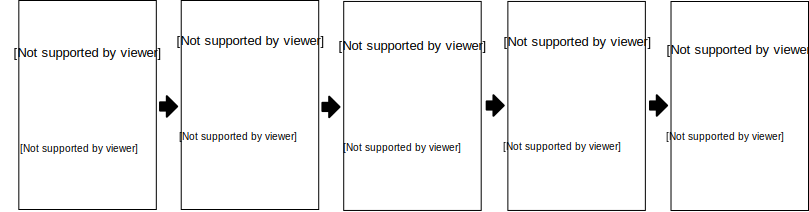
\includegraphics[scale=.75]{metodologia.pdf}}
	\caption{Etapas da Metodologia de Desenvolvimento de Pesquisa}
	\label{fig:metodologia_flow}
\end{figure}

\begin{itemize}
	\item \textbf{Pesquisa n�o sistem�tica sobre ontologias para experimentos:} foram realizado estudos n�o sistem�tico para encontrar trabalhos relacionados descrevendo ontologias para experimentos de ES e avalia��o de ontologia. Alguns estudos encontrados serviram de apoio a essa pesquisa, est�o descritos na Se��o \ref{sec:trabalhos_relacionados} ;
	
	\item \textbf{Desenvolvimento do projeto de ontologia para OntoExper-SPL:} trata sobre desenvolvimento da OntoExper-SPL, que incluiu realizar a escolha das tecnologias e ferramenta de constru��o de ontologia, como por exemplo o Prot�g�, envolver os \textit{stakeholders} no projeto com experi�ncia no dom�nio de experimenta��o, selecionar abordagens e modelos de ontologias relacionados, prototipa��o e diagrama��o do projeto;
	
	\item \textbf{Desenvolvimento do programa automatizado para povoar OntoExper-SPL:} refere-se ao processo de desenvolvimento do programa automatizado de povoamento da ontologia. Para isso foi necess�rio o uso de ferramentas, bibliotecas e linguagens de programa��o. Foram mais de 200 experimentos encontrados na literatura. Em seguida foi executado o programa de extra��o de dados, povoando a ontologia por meio dos metadados mais o programa de extra��o;
	
	\item \textbf{Avalia��o da qualidade e viabilidade do modelo:} refere-se ao estudo quali/quanti, com objetivo de avaliar a qualidade da OntoExper-SPL. Para isso foi elaborado um question�rio com oito crit�rios de qualidade, enviado para especialistas responderem, e posteriormente realizada uma an�lise estat�stica das respostas, bem como pontos de melhorias encontrados durante a avalia��o;
	
	\item \textbf{Desenvolvimento do prot�tipo de sistema de recomenda��o como prova de conceito:} ap�s processar os indiv�duos na OntoExper-SPL. Foi elaborado como prova de conceito, um prot�tipo de sistema de recomenda��o utilizando o modelos de recomenda��o \textit{Collaborative Filtering}, al�m de \textit{frameworks} e linguagens de programa��o.
\end{itemize}


\section{Organiza��o do texto}

Este cap�tulo apresentou a contextualiza��o desta disserta��o, a motiva��o e a justificativa, objetivos e metodologia. O restante da disserta��o est� estruturado da seguinte forma: o Cap�tulo \ref{sec:fundamentacao_teorica} apresenta a Fundamenta��o Te�rica sobre LPS, experimentais e quasi-experimentos em ES, qualidade de experimentos e quasi-experimentos em ES, Ontologias e Sistemas de Recomenda��o; o Cap�tulo \ref{sec:ontologia} apresenta uma Ontologia para Experimentos em LPS - OntoExper-SPL, destacando desde a concep��o ao povoamento da ontologia proposta e uma pr�-an�lise de pontos de falha da ontologia; o Cap�tulo \ref{sec:avaliacao} apresenta uma avalia��o quantitativa sobre a qualidade da OntoExper-SPL por especialistas da �rea; o Cap�tulo \ref{sec:recsys} apresenta um sistema de recomenda��o para experimentos em LPS, usando como modelo de dados a OntoExper-SPL; e o Cap�tulo \ref{sec:conclusao} apresenta as considera��es finais acerca deste projeto de disserta��o de mestrado, bom como as suas contribui��es, limita��es e trabalhos futuros.

\chapter{Fundamenta��o Te�rica}
\pagestyle{plain}
\label{sec:fundamentacao_teorica}


\section{Considera��es Iniciais}
\label{sec:fundamentos_concidaracoes_iniciais}


Este cap�tulo apresenta conceitos importantes sobre a fundamenta��o te�rica, necess�rias para a compreens�o desta pesquisa como LPS, experimento e \textit{quasi}-experimento em ES, qualidade de experimentos e \textit{quasi}-experimento em ES, ontologia, sistemas de recomenda��o e trabalhos relacionados. Dessa forma a estrutura deste cap�tulo fica, na Se��o \ref{sec:linha_de_produto_software} apresenta os principais pontos de LPS e variabilidades; na Se��o \ref{sec:experimentos_em_engenharia_de_software} � apresentado uma vis�o geral de experimento e \textit{quasi}-experimento em ES; na Se��o \ref{sec:qualidade_de_experimento_em_engenharia_de_software} s�o apresentados infroma��es preliminares sobre qualidade de experimentos e \textit{quasi}-experimento em ES; A Se��o \ref{sec:fundamentos_ontologia} descreve os fundamentos sobre o que � uma ontologia e sua finalidade; na Se��o \ref{sec:sistema_de_recmendacao} s�o apresentados os principais modelos para implementa��o de sistemas de recomenda��o, os tradicionais, e voltado para ES; Se��o \ref{sec:trabalhos_relacionados} s�o discutidos os trabalhos relacionados; e na Se��o \ref{sec:fundamentos_concidaracoes_finais} s�o apresentadas as Considera��es finais deste cap�tulo.


\section{Linha de Produto de Software}
\label{sec:linha_de_produto_software}

Uma Linha de Produto de Software (LPS) � um conjunto de produtos que endere�am a um determinado segmento de mercado ou miss�o particular \cite{northrop2007framework}. Esse conjunto de produtos tamb�m � denominado fam�lia de produtos, no qual os membros desta fam�lia s�o produtos espec�ficos gerados a partir da reutiliza��o de uma infraestrutura comum, denominada n�cleo de artefatos (\textit{Core assets}). 

O n�cleo de artefatos � composto por um conjunto de caracter�sticas comuns chamadas de similaridades, e caracter�sticas vari�veis chamadas de variabilidades \cite{van2007product}. Este n�cleo forma a base da LPS que determina a Arquitetura de uma LPS, que s�o eles, componentes reus�veis, modelos de dom�nios, requisitos da LPS, planos de testes e modelos de caracter�sticas de variabilidades.

O modelo de caracter�sticas cont�m todas as caracter�sticas de uma LPS e os seus inter-relacionamentos. De acordo com \citeauthor{apel2013analytic}, "uma caracter�stica � um comportamento caracter�stico ou vis�vel ao usu�rio final de um sistema de software". Uma caracter�stica pode ser obrigat�ria, opcional ou alternativa. O modelo de caracter�sticas representa as variabilidades e as variantes de uma LPS \cite{apel2013analytic}.

\begin{itemize}
	\item Variabilidades s�o descritas por: ponto de varia��o que permite a resolu��o de variabilidades em artefatos gen�ricos de uma LPS, e; 
	\item Variantes s�o representadas pelos: possess�veis elementos que podem ser escolhidos para resolver um ponto de varia��o.
\end{itemize}

Restri��es entre variantes, estabelecem os relacionamentos entre uma ou mais variantes, com o objetivo de resolver seus respectivos pontos de varia��o ou variabilidade em um dado tempo de resolu��o \cite{halmans2003communicating}.

O \textit{MobileMedia} � um exemplo did�tico de LPS, o produto final � um software que gerencia as m�dias de um aparelho celular. O n�cleo de artefatos deve conter algumas das seguintes caracter�sticas, op��es de criar, visualizar, remover e editar a legenda da imagem. As caracter�sticas variantes opcionais podem ser, a capturar uma nova imagem, ordenar e favoritar imagens. As caracter�sticas variantes alternativas podem ser os diversos tamanhos de tela. O produto final deve possuir ao menos uma variante alternativa.

\begin{figure}[htb]
	\centering					
	{\includegraphics[scale=.33]{exemplo_lps_pt.png}}
	
	\caption{Um modelo de Caracter�sticas. Traduzido de \citet{sommerville2011software} }
	\label{fig:exemplo-lps}
\end{figure}

A \ref{fig:exemplo-lps} apresenta um grafo com o Modelo de Caracter�sticas da LPS \textit{MobileMedia}. As arestas com c�rculos preenchido representa as caracter�sticas pertencentes ao \textit{core asset}. As arestas com c�rculos vazios representam caracter�sticas opcionais. As arestas ligadas por um tri�ngulo, como as que saem do v�rtice Sele��o de M�dia, representam caracter�sticas alternativas, por exemplo, uma inst�ncia desta LPS deve possuir ao menos um tipo de sele��o de m�dia, seja ele, por Foto, M�sica ou V�deo. 

Uma inst�ncia deste exemplo teria as seguintes caracter�sticas no seu produto de software final:
\begin{itemize}
	\item Gerenciamento de �lbum; 
	\subitem Criar �lbum;
	\subitem Excluir Album;
	\item Gerenciamento de M�dia;
	\begin{itemize}
		\item Opera��es B�sicas
		\subitem Criar M�dia
		\subitem Excluir M�dia
		\subitem Editar Legenda M�dia			
		\item Favoritos;
		\subitem Marcar Favoritos
		\subitem Visualizar Favoritos			
	\end{itemize}
	\item Sele��o de M�dia;
	\subitem Foto
	\subitem Visualizar Foto
	\subitem Capturar Foto			
\end{itemize}

\citeauthor*{pohl2005software} desenvolveram o \textit{framework} para engenharia de LPS. O objetivo deste de \textit{framework} � incorporar os conceitos centrais da engenharia de linha de produto tradicional, proporcionando a reutiliza��o de artefatos e a customiza��o em massa por meio de variabilidades. O \textit{framework} est� dividido em dois processos, o de Engenharia de Dom�nio e o de Engenharia de Aplica��o, conforme apresentado na \ref{fig:framework-lps}.

\begin{itemize}
	\item \textbf{Engenharia de Dom�nio:} processo em que as similaridades e as variabilidades das LPSs s�o identificadas e realizadas. No qual, � composto de cinco subprocessos principais, sendo eles: Gerenciamento de Produto, Engenharia de Requisitos do Dom�nio, Projeto do Dom�nio, Realiza��o do Dom�nio e Teste de Dom�nio;

	\item \textbf{Engenharia de Aplica��o:} processo em que as aplica��es de uma LPS s�o constru�das por meio da reutiliza��o de artefatos de dom�nio, explorando as variabilidades de uma linha de produto. No qual, � composto pelos subprocessos: Engenharia de Requisitos da Aplica��o, Projeto da Aplica��o, Realiza��o da Aplica��o e Teste da Aplica��o.
\end{itemize}

\begin{figure}[htb]
	\centering					
	{\includegraphics[scale=.37]{framewor_lps.png}}
	
	\caption{\textit{Framework} de Engenharia de LPS (Pohl et al., 2005). Traduzido por Geraldi (2015) }
	\label{fig:framework-lps}
\end{figure}


\section{Experimentos e \textit{Quasi}-Experimento em Engenharia de Software}
\label{sec:experimentos_em_engenharia_de_software}

Existe uma diferen�a relevante entre experimento e \textit{quasi}-experimento, esta diferen�a est� relacionada a amostra do experimento. Quando se trata de um experimento a amostra � uma representa��o aleat�ria e v�lida de uma determinada popula��o, ou seja, a amostra � uma representa��o da popula��o. Quando se trata de \textit{quasi}-experimento a amostra n�o � aleat�ria e n�o representa sua popula��o. � dif�cil realizar experimentos em LPS, devido a dificuldade de determinar uma amostra representativa e aleat�ria da popula��o, pois normalmente estas amostras s�o pessoas \cite{wohlin2012experimentation}.

Por meio de um modelo te�rico entre dois ou mais fen�menos relacionados a fim de determinar se este modelo proposto pode ser considerado correto, se desenvolve o experimento onde relacionamos a causa e o efeito deste modelo. Assim, utiliza-se o modelo para criar uma hip�tese em rela��o �s mudan�as particulares nos fen�menos (a causa) que levar�o a mudan�as no outro (o efeito). Logo, o papel do experimento � testar a hip�tese para decidir se � verdadeira ou falsa \cite{kitchenham2015evidence}. A \ref{fig:experimento} apresenta � ideia de uma rela��o causa e efeito em teoria, na qual a parte superior � linha tracejada se encontra a teoria e, na parte inferior a observa��o \cite{wohlin2012experimentation}.

\begin{figure}[htb]
	\centering					
	{\includegraphics[scale=.37]{experimento.png}}
	
	\caption{Conceitos Essenciais de um Experimento. Traduzido de \citet{wohlin2012experimentation} }
	\label{fig:experimento}
\end{figure}

Um dos principais elementos de um experimento s�o as vari�veis dependentes e independentes. 

\begin{itemize}
	\item \textbf{Vari�veis independentes:} est�o associadas � causa e controladas como resultado das atividades do experimentador, tamb�m s�o chamadas de fatores que podem assumir valores denominados tratamentos;
	\item \textbf{Vari�veis dependentes:} est�o associadas ao efeito e resultam nas mudan�as que o experimentador realiza nas vari�veis independentes \cite{kitchenham2015evidence}. 
\end{itemize}

Segundo \citealt{kitchenham2015evidence}, existe uma caracter�stica dita fator de confus�o em experimentos de ES que envolvem seres humanos. Esse fator pode ser representado pela presen�a de algum elemento indesej�vel no estudo que dificulta distinguir entre duas ou mais causas poss�veis de um efeito que foi medido pela vari�vel dependente como, por exemplo, os n�veis de habilidade dos participantes e a extens�o de suas experi�ncias anteriores com o objeto experimental.

Em Engenharia de Software, especialmente em LPS, � dif�cil de se executar experimentos dado que estes devem possuir aleatoriedade completa em suas vari�veis. Isto se deve � dificuldade de alocar os participantes e/ou objetos a diferentes tratamentos de maneira aleat�ria, bem como, � falta de representatividade do n�mero de participantes em uma amostra da popula��o. Portanto, os experimentos realizados nesta �rea s�o, frequentemente, \textit{quasi}-experimentos, nos quais n�o h� aleatoriedade dos participantes e/ou dos objetos experimentais, em ES chamados de artefatos de software, podendo ser processos ou ferramentas \cite{wohlin2012experimentation}.

Segundo \citealt{wohlin2012experimentation} a realiza��o de um experimento pode ser dividido em um processo contendo cinco atividades, conforme apresentadas na \ref{fig:proc_exp} e descritas a seguir:

\begin{figure}[htb]
	\centering					
	{\includegraphics[scale=.37]{proc_exp.png}}
	
	\caption{Vis�o Geral do Processo Experimental. Traduzido de \citet{wohlin2012experimentation}}
	\label{fig:proc_exp}
\end{figure}


\begin{itemize}
	\item \textbf{Defini��o:} � a primeira atividade, onde define-se o problema, objetivo e metas do experimento. Caso n�o seja devidamente estabelecida, pode ocorrer retrabalho ou o experimento n�o pode ser utilizado para se estudar o que era almejado;

	\item \textbf{Planejamento:} � uma prepara��o de como o experimento ser� conduzido, em que ocorre a determina��o do contexto do experimento, a formula��o das hip�teses, sendo \textbf{hip�tese nula} que o experimentador espera rejeitar com a maior confian�a poss�vel e a \textbf{hip�tese alternativa} que se espera aceitar, a sele��o de vari�veis (dependentes e independentes), a sele��o dos participantes, o projeto do experimento, a instrumenta��o e a avalia��o da validade, dividida em quatro tipos, sendo \textbf{validade interna} refere-se ao relacionamento tratamento-resultado; \textbf{validade externa} apresenta a generaliza��o dos resultados a uma popula��o maior; \textbf{validade de \textit{constructo}} demonstra a rela��o entre a teoria e observa��o; e \textbf{validade de conclus�o} refere-se a como os experimentadores foram aptos de analisar os resultados de um estudo e se a forma como foi feita � apropriada \cite{kitchenham2015evidence}.

	\item \textbf{Opera��o:} essa atividade � composta da \textbf{prepara��o} dos participantes e dos materiais necess�rios (instrumenta��o); \textbf{execu��o} das tarefas pelos participantes de acordo com diferentes tratamentos e coleta dos dados; e \textbf{valida��o dos dados} pelo experimentador, verificando os dados informados pelos participantes, de forma que os resultados do experimento sejam v�lidos; 
	
	\item \textbf{An�lise e Interpreta��o:} os dados coletados na atividade anterior s�o analisados utilizando a estat�stica descritiva. Ap�s isso, � verificada a necessidade de redu��o do conjunto de dados, de forma a garantir que os dados representam uma informa��o correta e/ou esperada. Por fim, realiza-se o teste de hip�teses para avaliar estatisticamente se hip�tese nula p�de ser rejeitada. 
	
	\item \textbf{Apresenta��o e Empacotamento:} nessa atividade, os resultados s�o reportados, por exemplo, como artigos em confer�ncia e/ou peri�dico, relat�rios de tomada de decis�o e empacotados para permitir a replica��o do experimento, como material educativo, entre outros.
\end{itemize}

\section{Qualidade de Experimentos em Engenharia de Software}
\label{sec:qualidade_de_experimento_em_engenharia_de_software}

Segundo \citet{dieste2013challenges}, o conceito de qualidade de experimentos em ES pode ser visto em dois pontos de vista diferentes, o primeiro � considerar a qualidade como o resultado da validade interna de um bom experimento e o segundo � tornar a qualidade operacional assim como a quantidade de vieses nos resultados experimentais. Outro ponto colocado por \citeauthor{dieste2013challenges}, � a validade externa que tamb�m tem uma fun��o chave ao analisar se um experimento tem boa qualidade, por�m essa fun��o � contr�ria � validade interna.

Na \ref{tab:conceito_qualidade} s�o apresentadas as defini��es dos conceitos de qualidade citados anteriormente.

% Please add the following required packages to your document preamble:
% \usepackage{booktabs}
\begin{table}[]
	\centering
	\caption{Defini��es dos conceitos de qualidade em experimentos em Engenharia de
		Software. Traduzido de \citet{kitchenham2007large}}
	\label{tab:conceito_qualidade}
	\begin{tabular}{@{}lll@{}}
		\toprule
		Termo & Sin�nimo & Defini��o \\ \midrule
		Vi�s & Erro sistem�tico & \begin{tabular}[c]{@{}l@{}}Uma tend�ncia para produzir resultados \\ que partem sistematicamente de resultados \\ "verdadeiros". Resultados sem vi�s s�o\\ v�lidos internamente.\end{tabular} \\
		Validade Interna & Validade & \begin{tabular}[c]{@{}l@{}}O alcance em que o projeto e a condu��o \\ do estudo s�o poss�veis de evitar erro sistem�tico. \\ A validade interna � um pr�-requisito \\ para a validade externa.\end{tabular} \\
		Validade Externa & \begin{tabular}[c]{@{}l@{}}Generabilidade, \\ Aplicabilidade\end{tabular} & \begin{tabular}[c]{@{}l@{}}O alcance em que os efeitos observados no estudo \\ s�o aplic�veis fora do estudo.\end{tabular} \\ \bottomrule
	\end{tabular}
\end{table}

Segundo \citet{dieste2011systematic} os experimentos de boa qualidade s�o aqueles livres de vieses. O vi�s est� relacionado com a validade interna, por exemplo, qu�o bem os experimentos s�o planejados, executados e analisados \cite{dieste2013challenges}. Para minimizar os vieses existem alguns m�todos como, aleatoriza��o para criar grupos experimentais homog�neos, imparcialidade para alocar os indiv�duos. Desta forma os resultados podem ser analisados mesmo depois do experimento ter sido realizado com replica��es. Enquanto os experimentos de baixa qualidade seriam os que usam pouco ou nenhum dos m�todos citados \cite{dieste2011systematic}.

Como o vi�s n�o pode ser medido, existem algumas abordagens para avali�-lo. Os instrumentos de Avalia��o de Qualidade (AQ), s�o projetados para avaliar a validade interna e inferir a qualidade de experimentos, tais como, abordagens simples (question�rios), \textit{checklists} (cont�m ou n�o cont�m), escalas de qualidade, opini�o de especialista \cite{dieste2011systematic,dieste2013challenges,teixeira2014analise}.

Por outro lado a qualidade de um experimento em ES tamb�m pode ser avaliada considerando o projeto e an�lise dos experimentos, em termos de poder estat�stico, an�lise do tamanho de efeito (resultado), \textit{quasi}-experimentais e relat�rio de experimento \cite{kampenes2007quality}.

At� o momento n�o se tem conhecimento de trabalhos que tratam a qualidade de experimentos em �rea espec�fica de ES. Entretanto, foram recuperados alguns trabalhos, por meio de pesquisas n�o sistem�ticas, que est�o relacionados com a avalia��o de qualidade dos experimentos em Engenharia de Software, descritos a seguir:

\begin{itemize}
	\item \citet{kitchenham2007large} prop�em um \textit{checklist} de avalia��o de qualidade de experimentos em ES contendo cinquenta quest�es para avaliar a qualidade de experimentos, em que sugerem que os pesquisadores selecionam apenas as quest�es do \textit{checklist} mais adequadas ao contexto de suas pr�prias quest�es de pesquisa.
	
	\item \citet{kitchenham2015evidence} apresentam um \textit{checklist} de avalia��o de qualidade de experimentos em ES com nove quest�es, onde cada quest�o possui subquest�es	categorizadas em: (i) "Quest�es sobre objetivo", (ii) "Quest�es sobre o projeto, coleta de dados e an�lise do dados" e (iii) "Quest�es sobre o resultado do estudo".
	
	\item \citet{dieste2011systematic}  desenvolveram uma escala de qualidade para determinar a qualidade de experimentos, contendo dez quest�es baseadas nas cinco dimens�es de \citet{kitchenham2007large}, sendo: contexto experimental, projeto experimental, an�lise, interpreta��o dos resultados e apresenta��o dos resultados. As respostas de cada quest�o s�o "sim" ou "n�o".	
\end{itemize}


\section{Ontologia}
\label{sec:fundamentos_ontologia}

A palavra ontologia � formada por meio dos termos gregos ontos (ser) e logos (estudo, discurso), que engloba algumas quest�es abstratas como a exist�ncia de determinadas entidades, o que se pode dizer que existe, qual o significado do ser, etc. Segundo \citet{wolff1962philosophia}, ontologia � um ramo da filosofia que estuda a realidade e exist�ncia, ou o ser enquanto ser. Em outras palavras, � o estudo da descri��o de coisas do mundo real. Outro ponto de vista proposto por \citet{gruber1993ontology}, diz que ontologias s�o uma especifica��o formal de uma contextualiza��o e uma contextualiza��o � uma vis�o abstrata e simplificada do mundo.

Ontologia em Computa��o, Sistemas de Informa��o e Ci�ncia da Informa��o, � definida como um modelo de dados que representa um conjunto de conceitos dentro de um dom�nio e os relacionamentos entre estes. Uma ontologia � utilizada para realizar infer�ncia sobre os objetos do dom�nio. No cen�rio atual, as ontologia em ci�ncias da informa��o s�o utilizadas como uma forma de representa��o de conhecimento l�gico, possibilitando a infer�ncia de novos fatos com base nos dados armazenados na ontologia.

Uma ontologia define primitivas/diretrizes de um dom�nio de conhecimento, estas primitivas/diretrizes podem ser definidas como classes, atributos, propriedades e restri��es. Essas defini��es seguem o padr�o de representa��o conhecido como l�gica descritiva. A l�gica descritiva representa os conceitos de um dom�nio (chamado de \textbf{TBox} - \textit{Terminological Box}) separadamente dos indiv�duos (chamado de \textbf{ABox} - \textit{Assertion Box}) \cite{calvanese2005dl}. A l�gica descritiva � mais representativa e eficiente que a l�gica proposicional e a l�gica de predicados (usados em linguagens de programa��o l�gica, como Prolog).

Portanto uma ontologia para a representa��o de um conhecimento possui a seguinte estrutura: Uma base de conhecimento onde est�o os dois conjuntos de conhecimento terminol�gico (\textbf{TBox}) e o conjunto de conhecimento sobre objetos (\textbf{ABox}), seguido de um mecanismo de infer�ncia e uma aplica��o para atuar na manipula��o de informa��es extra�das do mecanismo de infer�ncia, A \ref{fig:estrct_onto} apresenta essa estrutura.

\begin{figure}[htb]
	\centering					
	{\includegraphics[scale=.7]{estrutura_ontologia.png}}
	
	\caption{Estrutura de uma Ontologia. Autor}
	\label{fig:estrct_onto}
\end{figure}

\begin{figure}[htb]
	\centering					
	{\includegraphics[scale=0.45]{exemplo_ontologia.png}}
	
	\caption{Exemplo de uma Ontologia para o dom�nio: Destino de Viagem. Autor}
	\label{fig:exemplo_ont}
\end{figure}

A \ref{fig:exemplo_ont} apresenta um exemplo de ontologia, por meio de um grafo, para o dom�nio: "destino de viagem". Os v�rtices ovais representam as classes, e os v�rtices retangulares representam os indiv�duos (inst�ncias da classe). As arestas comuns representa um relacionamento de classe e subclasse, as arestas tracejadas representam um relacionamento de propriedade, j� as arestas que come�am com um losango indica a defini��o de uma propriedade, especificando sua tipagem.


\section{Sistema de Recomenda��o}
\label{sec:sistema_de_recmendacao}

Os sistemas de recomenda��o s�o aplicativos de software que visam dar suporte para usu�rio na tomada de decis�es ao interagir com grandes espa�os de informa��o. Estes softwares recomendam itens de interesse para os usu�rios com base em prefer�ncias que tenham sido expressas explicitamente ou implicitamente \cite{ricci2011introduction}. Segundo \citet{mahmood2009improving} os sistemas de recomenda��o s�o t�cnicas ou ferramentas de software, que podem reduzir a sobrecarga de informa��es para os usu�rios, sugerindo itens, conte�dos ou servi�os, entre outros.

\subsection{Sistemas de Recomenda��o Tradicional}

Os sistemas de recomenda��o surgiram nos trabalhos extensivos das ci�ncias cognitivas, teoria de aproxima��o, recupera��o da informa��o e teoria de previs�es e tamb�m possuem influ�ncias das ci�ncias de administra��o e marketing \cite{allen2001econometric, murthi2003role}. O primeiro sistema de recomenda��o proposto foi o \textit{Tapestry}, nesse sistema criou-se um modelo mais usados em sistemas de recomenda��o, onde a recomenda��o de conte�do � auxiliada pela colabora��o de um grupo de pessoas, batizada como "filtragem  colaborativa". Neste trabalho, iniciou o desafio de casar corretamente os que dados recomendados com os usu�rios que o recebem, analisando o real relacionamento de interesse \cite{kwong1992dynamic, resnick1997recommender}.

% Podemos apresentar uma defini��o formal para sistema de recomenda��o da seguinte forma: 

% \newtheorem{mydef}{Defini��o}
% \begin{mydef}
% 	Seja $C$ o conjunto de todos os usu�rios de um determinado sistema, e seja $S'$ o conjunto de todos os poss�veis itens que podem ser recomendados como livros, filmes, restaurantes etc. Seja $u$ a fun��o utilidade que mede o qu�o �til � um determinado item s para um determinado usu�rio $c$, \textbf{\textit{u}:C x S $\rightarrow$ R}, onde $R$ � um conjunto totalmente ordenado segundo a fun��o utilidade. Ent�o, para cada usu�rio \textbf{\textit{c} $\in$ C}, procura-se um item \textbf{\textit{s'} $\in$ S} que maximiza a utilidade do usu�rio. Isto pode ser expressado pela equa��o \ref{eq:form_sis_rec}:
	
% 	\begin{equation}
% 	\label{eq:form_sis_rec}
% 	\forall c \in C, s'_{c} = argmax_{s \in S u(c, s)}
% 	\end{equation}
	
% 	Em um sistema de recomenda��o a utilidade de um item � geralmente representada por uma avalia��o que indica o quanto um determinado usu�rio gosta de um item. No entanto, conforme descrito na defini��o acima, a fun��o de utilidade pode ser uma fun��o arbitr�ria.
	
% 	Cada elemento dos usu�rios $C$ pode ser definido por um perfil que inclui as caracter�sticas do usu�rio, por exemplo, a sua idade, sexo, etc. No caso mais simples, o perfil pode conter um �nico elemento como um identificador �nico (ID). Da mesma forma, cada item de $S$ pode ser definido por um conjunto de caracter�sticas. Por exemplo, na recomenda��o de filmes, na qual $S$ � a cole��o de filmes, cada filme pode ser representado n�o apenas pelo seu ID, mas tamb�m pelo seu t�tulo, g�nero, diretor, ano de lan�amento, etc.
% \end{mydef}

Existem cinco abordagens mais usadas em sistemas de recomenda��o, tr�s tradicionais: Filtragem Colaborativa (\textit{Collaborative Filtering}), Filtragem Baseada em Conte�do (\textit{Content-based Filtering}) e Recomenda��o Baseada no Conhecimento (\textit{Knowledge-Based Recommendation}), e duas modernas: Sistemas de Recomenda��o H�bridos \textit{(Hybrid Recommender Systems}) e Sistemas de Recomenda��o usando Informa��es de Contexto (\textit{Context-aware Recommender Systems}). 

Dado que este trabalho trata o sistema de recomenda��o como uma prova de conceito para realiza��o de infer�ncia sobre a SMartOntology, estar� descrito a seguir somente o modelo implementado no projeto de sistema de recomenda��o.

\subsubsection{Collaborative Filtering}
\label{sec:collaborative_filtering}

A Filtragem Colaborativa baseia-se na id�ia de "boca-a-boca" em que a informa��o passada de pessoa a pessoa desempenha um papel importante ao tomar uma decis�o. Abstraindo, as pessoas s�o substitu�das pelos chamados vizinhos mais pr�ximos (NN) que s�o usu�rios com um padr�o de prefer�ncia ou comportamento semelhante ao usu�rio atual. \cite{robillard2010recommendation}. Filtragem Colaborativa depende de dois tipos diferentes de dados: (1) um conjunto de usu�rios e (2) um conjunto de itens. A rela��o entre usu�rios e itens � expressada principalmente em termos de \textit{ratings} fornecidos pelos usu�rios e explorados em futuras sess�es de recomenda��o para prever a classifica��o de um usu�rio \cite{robillard2010recommendation}.

% \begin{itemize}
% 	\item \textbf{\textit{Collaborative Filtering}:}
	
% 	\item \textbf{\textit{Content-based Filtering}:}
% 	A Filtragem Baseada em Conte�do tem como caracter�stica principal o pressuposto de interesses pessoais, por exemplo, os usu�rios interessados no t�pico de qualidade de experimentos em LPS normalmente n�o alteram seu interesse de um dia para outro, mas tamb�m estar�o interessados em um t�pico pr�ximo, como por exemplo experimentos em Sistema de Sistemas. Abstraindo, as abordagens de recomenda��o baseadas em conte�do s�o aplicadas, por exemplo, quando se trata da recomenda��o de sites (not�cias com conte�do semelhante em compara��o com o conjunto de not�cias j� consumidas) \cite{robillard2010recommendation}. Filtragem Baseada em Conte�do depende de dois tipos diferentes de dados: (i) um conjunto de usu�rios e (ii) um conjunto de categorias (ou palavras-chave) atribu�das ou extra�das dos itens (descri��es de itens). Os sistemas de recomenda��o de filtragem baseados em conte�do calculam um conjunto de itens que s�o mais parecidos com itens j� conhecidos pelo usu�rio atual \cite{robillard2010recommendation}.

% 	\item \textbf{\textit{Knowledge-Based Recommendation}:} 
% 	A recomenda��o baseada no conhecimento, baseia-se nos seguintes	dados b�sicos: (i) um conjunto de regras (restri��es) ou m�tricas de similaridade e (ii) um conjunto de itens. Dependendo dos requisitos do usu�rio, regras (restri��es) que descrevam quais itens devem ser recomendados. O usu�rio atual articula suas necessidades (prefer�ncias) em termos de especifica��es e propriedades de itens que s�o internamente bem representados em termos de regras (restri��es).
	
% 	\item \textbf{\textit{Hybrid Recommender System}:}
% 	S�o algoritmos que combinam \textit{Collaborative Filtering} com \textit{Content-based Filtering} e podem ser feitos de diversas formas diferentes, por exemplo, aplicando os dois separados e juntando os resultados depois, adicionando a sa�da de um ao outro ou unificando as duas abordagens em um �nico modelo. Alguns exemplos s�o as abordagens baseada em pesos, misturadas a cascatas \cite{jannach2010recommender}.
	
	
% 	\item \textbf{\textit{Context-aware Recommender Systems}:} 
% 	Existem casos de recomenda��es que n�o podem levar em considera��o somente os dados do item ou do usu�rio, como conte�do personalizado de um site de filmes, sites de viagens e at� sites de not�cias. A incorpora��o do contexto permite personalizar ainda mais a recomenda��o e criar experi�ncias realmente v�lidas ao usu�rio. Segundo \citet{rahman2013ide} \textit{Context-aware Recommender Systems}, segue as abordagens anteriores assumindo a exist�ncia de certos fatores contextuais como, por exemplo, o tempo e a localiza��o, que identificam o contexto no qual as recomenda��es s�o fornecidas. Eles assumem que cada um desses fatores contextuais podem ter uma estrutura. O fator Tempo, por exemplo, pode ser definido em termos de segundos, minutos, horas, dias, meses e anos. \citet{rahman2013ide} cita como classificar o contexto baseando-se nos seguintes aspectos, (i) o que um sistema de recomenda��o pode saber sobre esses fatores contextuais e (ii) como os fatores contextuais mudam ao longo do tempo. Desta forma podemos definir este tipo de sistema de recomenda��o pela formula \ref{eq:form_sis_rec_ca}
	
% 	\begin{equation}
% 		\label{eq:form_sis_rec_ca}
% 		f:User \times Item \times Context \rightarrow Rating
% 	\end{equation}

% \end{itemize}


\subsection{Sistema de Recomenda��o em Engenharia de Software}

Em Engenharia de Software (\textit{Recommendation System in Software Engineering} - RSSEs), sistemas de recomenda��o desempenham importantes fun��es a fim de ajudar a equipe de software a lidar com sobrecarga de informa��es, filtrando e fornecendo informa��es �teis. S�o ferramentas de software introduzidas especificamente para ajudar equipes de desenvolvimento de software e partes interessadas a lidar com a busca de informa��es em um determinado contexto em ES \cite{robillard2010recommendation}.

\citet{robillard2010recommendation} comenta que, em um ambiente de desenvolvimento de software aplicando ES existe um \textit{landscape} de informa��es sobre o projeto em desenvolvimento, e este espa�o de informa��es pode ser categorizados por:

\begin{itemize}
	\item C�digo fonte do projeto;
	\item Hist�ria do projeto;
	\item Arquivos de comunica��o;
	\item Depend�ncias de API em outras fontes;
	\item Ambiente de desenvolvimento;
	\item Logs de intera��o entre os usu�rios;
	\item Logs de execu��o e;
	\item A web.
\end{itemize}

Um RSSE pode trazer simultaneamente dois aspectos distintos: (i) novidade e surpresa, porque as RSSEs ajudam a descobrir novas informa��es e (ii) traz familiaridade e refor�o, pois as RSSEs suportam a confirma��o do conhecimento existente. Finalmente, referenciar uma tarefa e um contexto espec�ficos, distingue RSSEs de ferramentas de pesquisa gen�ricas, por exemplo, uma ferramentas de RSSR para ajudar os desenvolvedores a encontrar exemplos de c�digo fonte \cite{robillard2010recommendation}.

RSSE compreende tr�s componentes principais, (i) um mecanismo para coletar dados, (ii) um mecanismo de recomenda��o para analisar dados e gerar recomenda��es e (iii) uma interface de usu�rio para fornecer recomenda��es \cite{rahman2014towards}.

\begin{figure}[htb]
	\centering					
	{\includegraphics[scale=.5]{rsse.png}}
	
	\caption{Passos de Constru��o para um RSSE. Traduzido e Adaptado de \citet{maki2016systematic}}
	\label{fig:rsse}
\end{figure}

A \ref{fig:rsse} apresenta de forma geral como � constru�do um RSSE, partindo da entradas dos dados pelo \textit{input}, passando pela extra��o de contexto, seguindo para aplica��o de alguma t�cnica de recomenda��o, na qual sofre um infer�ncia do corpo de conhecimento (normalmente espec�fico para cada �rea de ES), depois segue para um processo de filtragem dos resultados, e como sa�da a recomenda��o em si.

Foi encontrado uma revis�o sistem�ticas (trabalho da \citealp{maki2016systematic}), que aborda m�todos e modelos de implementa��o de um RSSE apresentando v�rios aspectos de SR em ES, principalmente no tipo de corpo de conhecimento aplicado a RSSE. Nessa revis�o foi poss�vel identificar algumas �reas da ES que utiliza SR, apresentadas a seguir.

\begin{itemize}
	\item SR para explora��o c�digo fonte;
	\item SR para reuso de software;
	\item SR para refatora��o de c�digo fonte (por exemplo, \textit{class} em POO);
	\item SR para reuso de componentes de software;
	\item SR na explora��o de APIs;
	\item SR na depura��o de c�digo (\textit{debugging})
	\item SR na recomenda��o de agentes \textit{Agile}
	\item SR na descoberta de requisitos;
	\item SR na mudan�a do ciclo de vida;
	\item SR na evolu��o do ciclo de vida e;
	\item SR na busca de \textit{bugs}.
\end{itemize}

% Por meio deste estudo, foi poss�vel identificar em qual dom�nio de aplica��o da industria de ES est�o aplicando qual t�cnica de SR, apresentados na \ref{tab:tec_x_doman} a seguir.

% \begin{table}[]
% 	\centering
% 	\caption{Sum�rio de t�cnicas de recomenda��o em cada dom�nio, Traduzido e Adaptado de \citet{maki2016systematic} }
% 	\label{tab:tec_x_doman}
% 	\begin{tabular}{@{}llllllllll@{}}
% 		\toprule
% 		\multicolumn{1}{c}{\textbf{Dom�nios}} & \multicolumn{8}{c}{\textbf{T�cnicas}} & \multicolumn{1}{c}{\textbf{\begin{tabular}[c]{@{}c@{}}N�mero de \\ Refer�ncias\end{tabular}}} \\ \midrule
% 		& CBF & CF & KBF & Hibrido & IA & \begin{tabular}[c]{@{}l@{}}Redes \\ Sociais\end{tabular} & \begin{tabular}[c]{@{}l@{}}Info. de\\ Contexto\end{tabular} & \begin{tabular}[c]{@{}l@{}}Grupo de \\ agrega��o\end{tabular} &  \\ \midrule
% 		Governo & 1 & 5 & 1 & 5 & 4 &  &  &  & 9 \\
% 		Neg�cios &  & 1 & 3 & 3 & 4 &  &  &  & 5 \\
% 		Comercio & 3 & 1 & 4 & 1 & 4 & 2 &  &  & 8 \\
% 		Livraria & 2 & 2 &  & 3 & 1 &  &  &  & 6 \\
% 		Escolas & 2 &  & 11 &  & 1 &  &  &  & 10 \\
% 		Turismo & 5 & 9 & 9 & 9 & 2 & 2 & 11 &  & 18 \\
% 		Pesquisa & 9 & 16 & 6 & 15 & 3 & 1 & 1 &  & 27 \\
% 		\begin{tabular}[c]{@{}l@{}}Grupo de \\ Atividade\end{tabular} & 9 & 5 & 2 & 5 & 8 &  &  & 2 & 21 \\
% 		\textbf{Total} & \textbf{31} & \textbf{39} & \textbf{36} & \textbf{41} & \textbf{27} & \textbf{5} & \textbf{12} & \textbf{2} & \textbf{104} \\ \bottomrule
% 	\end{tabular}
% \end{table}

\section{Trabalhos Relacionados}
\label{sec:trabalhos_relacionados}

Durante uma revis�o n�o sistem�tica (\textit{ad hoc}) da literatura foram encontrados alguns estudos que propuseram abordagens para representar formalmente dados sobre experimentos em ES. A revis�o da literatura mostrou que a maioria dos estudos focou e representar todo o dom�nio do ES, ou experimentos em geral, esse fator � um agravante para elabora��o dos modelos, pois, � quantidade de detalhes pode variar significativamente. Estes trabalhos est�o descritos a seguir. A contribui��o deles � discutida ao final desta sess�o.

Durante nossa revis�o de literatura encontramos: \cite{garcia2008ontology} Ontologia para Experimentos Controlados em Engenharia de Software, \cite{scatalon2011packaging} Empacotando Experimentos Controlados Usando uma Abordagem Evolutiva Baseada em Ontologia (S), \cite{da2012foundational} Uma Ontologia Fundamental para Apoiar Experimentos Cient�ficos, \cite{blondet2016ode} ODE: uma Ontologia para Projeto Num�rico de Experimentos, \cite{soldatova2006ontology} Uma Ontologia de Experimentos Cient�ficos, \cite{gelernter2016challenges} Desafios na Avalia��o de Ontologia, \cite{cruzes2007extracting} Extraindo Informa��es da Engenharia de Software Experimental pap�is. No entanto, todos esses trabalhos n�o tratam experimentos de LPS.

O trabalho de Garcia et al. \cite{garcia2008ontology}, Poveda-Villal�n et al. \cite{scatalon2011packaging} e Cruz et al. \cite{da2012foundational} se destaca em nosso contexto por propor e modelar ontologias espec�ficas para experimentos em engenharia de software. O trabalho de \cite{garcia2008ontology} prop�e, atrav�s de diagramas de classes UML, uma ontologia para experimentos controlados em engenharia de software denominada EXPEROntology. Com o objetivo de ser uma ferramenta de transfer�ncia de conhecimento para auxiliares de pesquisadores e revisores, al�m de propor meta-an�lises, conduzir e avaliar experimentos controlados. O trabalho de Poveda-Villal�n et al. \cite{scatalon2011packaging} � uma evolu��o do trabalho de Garcia et al. \cite{garcia2008ontology}, mas focado na evolu��o desta ontologia proposta. O trabalho de Cruz et al. \cite{da2012foundational} apresenta uma ontologia chamada OVO (Open onVence Ontology) na qual � inspirada por tr�s teorias: (i) O ciclo de vida de experimentos cient�ficos, (ii) Open Provent (OPM) e (iii) Unified Foundational Ontology ( OVNI) Este modelo OVO pretende ser uma refer�ncia para modelos conceituais que podem ser usados ??por pesquisadores para explorar a sem�ntica de metadados.

Por outro lado, os trabalhos de Blondet et al. \cite{blondet2016ode} e Soldatova e King \cite{soldatova2006ontology} tratam ontologias no contexto geral de experimentos. O trabalho de Blondet et al. \cite{blondet2016ode} traz uma proposta de ontologia para DoE (Designs of Experiments) para apoiar as decis�es de processo sobre o DoE. O trabalho de Soldatova e King \cite{soldatova2006ontology} prop�e a ontologia da EXPO que � uma mediana da ontologia SUMO (Suggested Upper Merged Ontology). Esta ontologia visa especificar os experimentos formalizando e generalizando os conceitos de design, metodologias e representa��o de resultados. Este trabalho � o �nico que usa o modelo OWL-DL para representar a ontologia.

O trabalho de Gelernter e Jha \cite{gelernter2016challenges} d� uma vis�o geral sobre os desafios de avaliar uma ontologia, mas n�o trata da ontologia para experimentos.

Finalmente, o trabalho de Cruzes et al. \cite{cruzes2007extracting} trata de uma t�cnica para extrair meta-informa��o de experimentos em engenharia de software, entendemos que este assunto est� relacionado a este artigo, pois estaremos gerando atrav�s da ontologia proposta diversos metadados sobre experimentos em SPL.

Apesar de n�o haver um padr�o para modelar o conhecimento de experimenta��o em ES a literatura apresenta estrat�gias diferentes neste sentido, como pode ser notado nos trablahos de \cite{garcia2008ontology} e \cite{scatalon2011packaging}. Desse modo a modelagem de otologia de para este trabalho ser� aplicado para experimento em LPS, de tal modo que, ser� poss�vel fazer infer�ncia de LPS na ontologia e extrair informa��es. Assim tais trabalhos relacionados s�o fundamentais para realiza��o deste trabalho de mestrado.

At� o momento n�o h� trabalhos de sistema de recomenda��es para voltados a experimentos em ES, e nem em LPS. Outros trabalhos relacionados mais pr�ximos j� foram apresentado na Se��o \ref{sec:qualidade_de_experimento_em_engenharia_de_software} e n�o s�o objetos de evolu��o de experimento gerais em ES.


\section{Considera��es Finais}
\label{sec:fundamentos_concidaracoes_finais}

Este cap??tulo apresentou os conceitos essenciais sobre a abordagem de LPS como variabilidades e variantes, apresentando o \textit{MobileMedia} como exemplo para melhor entendimento dos conceitos, bem como o framework de engenharia de LPS proposto por /cite{Pohl et al. (2005)}?. 

Em rela��o � experimenta��o em ES, foi apresentado os principais elementos como as vari�veis dependentes e independentes, as atividades de um processo experimental como defini��o, planejamento, opera��o, an�lise e interpreta��o, apresenta��o e empacotamento. Sobre qualidade de experimentos em ES foi introduzido conceitos preliminares sobre a qualidade de experimentos como vi�s, validade interna e validade externa e tamb�m algumas abordagens para aplicar uma avalia��o de qualidade sobre os experimentos em ES. 

Quando foi tratado de ontologia, foi descrito a defini��o universal de ontologia e a defini��o voltada para computa��o. Nessa temos que a ontologia � uma modelagem formal de dados para representa��o de um determinado dom�nio, para isso, existe a \textit{TBox} para representar a l�gica descritiva e a \textit{ABox} para representar os indiv�duos pertencentes a ontologia. Assim como em LPS foi apresentado um exemplo (Destino de Viagem) para facilitar o entendimento dos conceitos abordados. 

Sobre sistemas de recomenda��o foram apresentados os modelos b�sico de sistemas de recomenda��o tradicionais, como \textit{collaborative filtering} e \textit{content-based filtering}. Na sequ�ncia foi apresentado como os sistemas de recomenda��o s�o tratados na ES e alguns exemplos de aplica��o.

Por fim, temos os trabalhos relacionados tra�ando um paralelo de modelagem para representa��o do dom�nio de LPS eom este trabalho.

No pr�ximo cap�tulo, ser� apresentado uma ontologia para experimento em LPS, a SMartOntology.


\chapter{Uma Ontologia para Experimentos em LPS - OntoExper-LPS}
\pagestyle{plain}
\label{sec:ontologia}


\section{Considera��es Iniciais}
\label{sec:concidaracoes_iniciais}

Este cap�tulo apresenta a elabora��o da proposta de ontologia OntoExper-LPS, sua concep��o, a constru��o do projeto, exemplos de aplica��o, uma breve avalia��o emp�rica e considera��es finais. Dessa forma a estrutura deste cap�tulo fica, na Se��o \ref{sec:concepcao} apresenta o processo de concep��o do modelo seguindo a tipologia de \cite{almeida2003visao} bem como a elabora��o de um grafo como modelagem inicial da ontologia, seguindo como base um modelo conceitual clusterizado sobre elementos experimentais de ES em LPS; na Se��o \ref{sec:projeto} foi desenvolvido o projeto da OntoExper-LPS para se obter modelo ontol�gico, foi utilizado como tecnologia base OWL (\textit{Ontology Web Language}) juntamente com a Ferramenta Prot�g�, o resultado final foi um artefato do tipo OWL contendo toda modelagem de classes, subclasses, propriedades de objeto e propriedades dos dados, al�m da modelagem, foi criado nesta se��o, um programa automatizado para povoar a ontologia utilizando os metadados levantados pelo GReater, este programa conta com a utiliza��o da linguagem de programa��o Python e a biblioteca OwlReady2; na Se��o \ref{sec:exemplo} foi elaborado uma consulta SPARQL para demonstrar como interagir com a ontologia e uma breve explica��o deste procedimento; na Se��o \ref{sec:avaliacao_empirica} foi realizado uma avalia��o emp�rica do modelo, por meio da ferramenta OOPS! que avalia pontos de falha do modelo, nesta se��o discutimos como estes ponto de falham impacta no modelo proposto por este trabalho.


\section{Concep��o}
\label{sec:concepcao}

Com base na tipologia proposta por \cite{almeida2003visao} definimos o tipo da ontologia proposto neste trabalho, descrito na Tabela \ref{tab:tipo-modelo-ontologia}. Todas as tipologias para ontologias podem ser encontradas no Ap�ndice \ref{apendice:a-tipologia}

Ou seja, podemos tipificar o modelo proposto como; \textbf{quanto � fun��o:} � uma ontologia de dom�nio, \textbf{quanto ao grau de formalismo:} � uma ontologia semi formal, \textbf{quanto � aplica��o:} � uma ontologia de especifica��o, \textbf{quanto � estrutura:} � uma ontologia de dom�nio e \textbf{quanto ao conte�do:} � tanto uma ontologia para modelagem de conhecimento quanto para aplica��o de dom�nio.

Tamb�m foi aplicado o seguinte processo de elabora��o da ontologia, seguindo os processos proposto por \cite{fernanda2007modelagem}:

\begin{itemize}
	\item Defini��o e estrutura��o dos termos por meio de classes;  
	\item Estabelecimento de propriedades (atributos) inerentes ao conceito representado por um termo;
	\item Povoamento da estrutura que satisfa�am um conceito e as suas propriedades;  
	\item Estabelecimento de rela��es entre os conceitos;
	\item Elabora��o de senten�as para restringir infer�ncias de conhecimento baseadas na estrutura.
\end{itemize}

\begin{landscape}
	\topskip0pt
    \vspace*{\fill}
	\begin{table}[]
		\label{tab:tipo-modelo-ontologia}
		\caption{Tipagem da ontologia proposta}
		\centering
		\begin{tabular}{@{}lll@{}}
			\toprule
			Abordagem & Classifica��o & Descri��o \\ \midrule
			\begin{tabular}[c]{@{}l@{}}Quanto � fun��o \\ Mizoguchi; Vanwelkenbuyse \\ n; Ikeda (1995)\end{tabular} & Ontologias de dom�nio & \begin{tabular}[c]{@{}l@{}}Reutiliz�veis no dom�nio, fornecem vocabul�rio \\ sobre conceitos e seus relacionamentos, sobre as \\ atividades e regras que os governam.\end{tabular} \\
			\begin{tabular}[c]{@{}l@{}}Quanto ao grau de formalismo \\ Uschold; Gruninger (1996)\end{tabular} & Ontologias semi informais & \begin{tabular}[c]{@{}l@{}}Expressa em linguagem natural de forma restrita \\ e estruturada.\end{tabular} \\
			\begin{tabular}[c]{@{}l@{}}Quanto � aplica��o \\ Jasper; Uschold (1999)\end{tabular} & \begin{tabular}[c]{@{}l@{}}Ontologias como \\ especifica��o\end{tabular} & \begin{tabular}[c]{@{}l@{}}Cria-se uma ontologia para um dom�nio, a qual � \\ usada para documenta��o e manuten��o no \\ desenvolvimento de softwares.\end{tabular} \\
			\begin{tabular}[c]{@{}l@{}}Quanto � estrutura \\ Haav; Lubi (2001)\end{tabular} & Ontologias de dom�nio & \begin{tabular}[c]{@{}l@{}}Descrevem o vocabul�rio relacionado a um dom�nio, \\ como, por exemplo, medicina ou autom�veis\end{tabular} \\
			\multirow{3}{*}{\begin{tabular}[c]{@{}l@{}}Quanto ao conte�do \\ Van-Heijist; Schreiber; \\ Wielinga (2002)\end{tabular}} & \begin{tabular}[c]{@{}l@{}}Ontologias de modelagem\\ do conhecimento\end{tabular} & \begin{tabular}[c]{@{}l@{}}Especificam conceitua��es do conhecimento, t�m uma \\ estrutura interna semanticamente rica e s�o refinadas\\ para uso no dom�nio do conhecimento que descrevem\end{tabular} \\
			& Ontologias de aplica��o & \begin{tabular}[c]{@{}l@{}}Cont�m as defini��es necess�rias para modelar o \\ conhecimento em uma aplica��o.\end{tabular} \\
			& Ontologias de dom�nio & \begin{tabular}[c]{@{}l@{}}Expressam conceitua��es que s�o espec�ficas para \\ um determinado dom�nio do conhecimento.\end{tabular} \\ \bottomrule
		\end{tabular}
	\end{table}
	\vspace*{\fill}
\end{landscape}

O primeiro passo foi desenvolver um grafo como modelo inicial da ontologia OntoExper-LPS, o objetivo principal foi de externalizar id�ias iniciais do modelo e visualizar hierarquias e relacionamentos entre os termos inicialmente propostos.

\begin{figure}[]
	\centering 
	\includegraphics[scale=0.5]{grafo-inicial.pdf}
	\caption{Grafo inicial da proposta de ontologia.}
	\label{figure:graph-all-class}
\end{figure}

A \ref{figure:graph-all-class} representa este modelo inicial contendo a defini��o principal dos termos para o experimento, Experimento SPL, Documenta��o, Template, Avalia��o, Discuss�o, An�lise, Execu��o e Planejamento. Em seguida evolu�mos para poss�veis termos de mais baixa hierarquia, que est�o definidas a seguir:


\begin{itemize}
	\item Documenta��o;
	\begin{itemize}
		\item Dom�nio em LPS;
		\item \textit{Abstract}:
		\begin{itemize}
			\item Palavra Chave; 
			\item Limita��es;
			\item Conclus�es;
			\item Resultados;
			\item M�todos; e
			\item Objetivos.			
		\end{itemize}
		\item Introdu��o:
		\begin{itemize}
			\item Contexto;
			\item Objetivo da Pesquisa (GQM); e
			\item Quest�es do Problema.
		\end{itemize}
		\item Trabalhos Relacionados:
		\begin{itemize}
			\item Estudos Relacionados;
			\item Tecnologia sob Investiga��o;
			\item Tecnologia Alternativa; e
			\item Relev�ncia na Pr�tica.
		\end{itemize} 
		\item Template:
		\begin{itemize}
			\item Observa��o.
		\end{itemize}
		\item Refer�ncias;
		\item Agradecimentos;
		\item Conclus�o; e
		\item Ap�ndice.
	\end{itemize}
	\item Planejamento:
	\begin{itemize}
		\item Contexto:
		\begin{itemize}
			\item Local.
		\end{itemize} 
		\item Unidade Experimental:
		\begin{itemize}
			\item Sele��o dos Participantes;
		\end{itemize} 
		\item Material Experimental:
		\begin{itemize}
			\item Artefatos de SPL;
			\begin{itemize}
				\item Fonte
			\end{itemize} 
		\end{itemize} 
		\item Projeto Experimental;
		\item Par�metros;
		\item Vari�veis;
		\item Procedimentos;
		\item Objetivo;
		\item Hip�teses;
		\item Tarefas;
		\item An�lises de procedimentos;
	\end{itemize} 
	\item Execu��o:
	\begin{itemize}
		\item Prepara��o:
		\begin{itemize}
			\item Projeto Piloto;
		\end{itemize}	 
		\item Execu��o; e
		\item Desvio do Planejamento;
	\end{itemize}
	\item An�lise:
	\begin{itemize}
		\item Tipo de An�lise:
		\begin{itemize}
			\item Meta An�lise
			\item Tipo de An�lise de Hip�tese;
		\end{itemize} 
		\item Teste de Hip�tese:
		\begin{itemize}
			\item P-value
		\end{itemize} 
		\item Estat�stica Descritiva;
		\item An�lise qualitativa;
		\item Prepara��o do \textit{Dataset};
	\end{itemize} 
	\item Discuss�o:
	\begin{itemize}
		\item Amea�as a Validade:
		\begin{itemize}
			\item Amea�a a Validade em LPS.
		\end{itemize} 
		\item Avalia��o dos Resultados;
		\item Infer�ncias;
		\item Li��es Aprendidas;
	\end{itemize}	 
	\item Empacotamento:
	\begin{itemize}
		\item Pacote Experimental.
	\end{itemize} 
	\item Avalia��o:
	\begin{itemize}
		\item Abordagem de Avalia��o.
	\end{itemize} 

\end{itemize}

Esta modelagem inicial da ontologia foi baseada no trabalho de mapeamento sistem�tico de experimentos em LPS de \cite{Furtado2018}, por meio de uma an�lise explorat�ria dos dados levantados nesse mapeamento, foi poss�vel usa-lo como guia de informa��es e metadados de ESE em LPS.

O mapeamento sistem�tico levou em considera��o o temple experimental de Wohlin, que traz cinco fases para elabora��o de ESE, s�o eles, Defini��o, Planejamento, Opera��o, An�lise e Interpreta��o \cite{wohlin2012}.

\begin{landscape}
	\topskip0pt
    \vspace*{\fill}
	\begin{figure}[]
		\centering 
		\includegraphics[scale=.65]{modelo-conceitual-clusterizado.pdf}
		\caption{Modelo Conceitual Clusterizado.}
		\label{figure:conceptual_model_clustering}
	\end{figure}
	\vspace*{\fill}
\end{landscape}

A \ref{figure:conceptual_model_clustering}, apresenta uma modifica��o do modelo conceitual original, elaborada no trabalho de \cite{Furtado2018}, onde foi aplicado a clusteriza��o separando cada cluster para cada fase do template experimental de Wohlin. Esta clusteriza��o foi necess�ria para compreens�o mais abstrata das rela��es entre os termos do dom�nio levantados no modelo conceitual original e as fases do template do Wholin. Dessa forma foi poss�vel validar cada termo do grafo inicialmente proposto.
	
Em seguida, um diagrama de classes foi elaborado para representar de uma maneira mais intuitiva a modelagem inicial, realizada com grafos. O objetivo � transformar cada termos do grafo em uma classe do conceito de Orienta��o a Objetos. Nessa representa��o, a modelagem da \textit{TBox}, ou seja, a rela��o entre os termos (classes) e suas propriedades (atributos) ficou mais clara. Essa forma de representa��o destacou a rela��o principal quando definimos a composi��o da classe Experiment e ExperimentSPL em quase todas as outras subclasses. Nesta representa��o tamb�m ficou expl�cita a tipifica��o das propriedades, para posteriormente executar a inser��o da \textit{ABox} na modelagem.

A \ref{figure:class_diagram_ontology} apresenta o diagrama de classe gerado para o modelagem da ontologia. Este diagrama representa todas composi��es de classes que existe com Experiment e ExperimentSPL, bem como as rela��es hier�rquicas como por exemplo, ExperimentSPL � uma subclasse de Experiment.

\begin{landscape}
	\topskip0pt
    \vspace*{\fill}
	\begin{figure}[]
		\centering
		\includegraphics[scale=.3]{class-diagram-ontology.png}
		\caption{Diagrama de Classe para proposta da modelagem da ontologia.}
		\label{figure:class_diagram_ontology}
	\end{figure}
	\vspace*{\fill}
\end{landscape}

Posteriormente, foi utilizada a ferramenta Prot�g� para constru��o oficial da ontologia, seguindo os padr�es OWL.


\section{Projeto}
\label{sec:projeto}

Definimos a cria��o da ontologia usando a tecnologia OWL, foram constru�das as classes e subclasses para representar os elementos da ontologia, por meio da ferramenta Prot�g�.

\subsection{Modelagem com Prot�g�}
\label{sec:protege}

A ferramenta Prot�g� � um ambiente de desenvolvimento voltado para cria��o de ontologias. Ela disp�e de uma interface gr�fica para edi��o de ontologias e uma arquitetura para a cria��o de ferramentas baseadas em conhecimento. Pode ser usada tanto por, desenvolvedores de sistema, como por especialistas em dom�nio, para criar bases de conhecimento, permitindo representar facilmente o conhecimento de uma �rea. Este editor � capaz de tratar classes, com sua defini��o e exemplos, simultaneamente propriedades de objetos e de dados \cite{DBLP:journals/aimatters/Musen15}.

% O padr�o OWL foi usado no OntoExper-LPS para definir todos os elementos, classes, propriedades de objetos e dados.

Fazendo uma analogia ao diagrama de classe, no Prot�g�, as classes, os atributos de classes e seus relacionamentos est�o em um contexto de entidades. As classes e hierarquias s�o definidos na aba \textbf{Classes}, os relacionamentos s�o definidos na aba \textbf{Propriedades de Objetos} e os atributos s�o definidos na aba \textbf{Propriedade dos Dados}.

Definimos nossas entidades com base do diagrama de classe constru�do na fase de concep��o, com a seguinte estrutura (i) defini��o de classes (ii) defini��o das propriedades de objetos, (iii) defini��o das propriedades dos dados.

\subsubsection{Defini��o de classes}

No Prot�g�, definimos uma classe raiz chamada \textit{Thing} na qual todas as outras classes s�o filhas dela. A \ref{figure:class_defition_protege} apresenta a defini��o da classe Experiment dentro do modelo, neste momento a defini��o � composta pelo nome da classe e seus principais relacionamentos \textit{(Equivalent To e SubClass Of)}.

\begin{figure}[htb]
	\centering 
	\includegraphics[scale=.5]{entidades-protege.png}
	\caption{Defini��o da classe Experiment no Prot�g�.}
	\label{figure:class_defition_protege}
\end{figure}

\subsubsection{Defini��o das propriedades de objetos}

No Prot�g�, definimos uma propriedade de objeto raiz chamada \textit{topObjectProperty} na qual todas as outras propriedades s�o filhas dela. A \ref{figure:object_prop_defition_protege} apresenta a defini��o de propriedade de objeto para propriedade \textit{documentation}, neste momento a defini��o � composta pelo nome da propriedade e seus relacionamentos com classes, Dom�nio \textit{(Domains)} e Alcance \textit{(Ranges)}.

\begin{figure}[!htb]
	\centering 
	\includegraphics[scale=.5]{entidades-protege-object-properties.png}
	\caption{Defini��o da propriedade de objeto documentation no Prot�g�.}
	\label{figure:object_prop_defition_protege}
\end{figure}

\subsubsection{Defini��o das propriedades dos dados}

No Prot�g�, definimos uma propriedade de dados raiz chamada \textit{topDataProperty} na qual todas as outras propriedades s�o filhas dela. Para cada Propriedade de dado definimos um conjunto de classes de seu Dom�nio e um conjunto de tipos de dados (predefinido) de seu Alcance, por exemplo, a propriedade de dado \textit{nameSPLUsed} possui como classe de dom�nio ExperimentSPL e como alcance um \textit{xsd:string}. A \ref{figure:data_prop_defition_protege} apresenta a defini��o de propriedade de dado para chamada \textit{nameSPLUsed}, neste momento a defini��o � composta pelo nome da propriedade e seus relacionamentos, Dom�nio (uma classe) e Alcance (uma tipagem).

\begin{figure}[htb]
	\centering 
	\includegraphics[scale=.5]{entidades-protege-data-properties.png}
	\caption{Defini��o da propriedade de dado nameSPLUsed no Prot�g�.}
	\label{figure:data_prop_defition_protege}
\end{figure}

\subsubsection{Artefato gerado pelo Prot�g�}

Ao final, o Prot�g� gera um arquivo \textit{.owl} contendo toda a defini��o do modelo. A \ref{figure:graph_ontology_model} fornece uma vis�o geral no formato de grafo do projeto, contendo todas as classes. Usamos a ferramenta WebVOWL \cite{lohmann2016visualizing} para gerar essa vis�o.

\begin{figure}[htb]
	\centering 
	\includegraphics[scale=.6]{ontology-populate-valid-owl-2.pdf}
	\caption{Grafo da modelagem da ontologia - gerado pelo WbVOWL.}
	\label{figure:graph_ontology_model}
\end{figure}

\subsection{Povoamento com Python}
\label{sec:python}

A pr�xima etapa, ap�s a modelagem da ontologia, foi inserir os indiv�duos na mesma, ou seja, popular a ontologia para realiza��o de infer�ncias futuras. Apesar do Prot�g� ter capacidade para realizar essa opera��o, optamos por utilizar um script para realizar tal tarefa, visto que, no Prot�g� o processo de inserir indiv�duos na ontologia � realizado de modo manual, por meio do menu \textit{Individuals by Class}, onde � preciso selecionar propriedade por propriedade para cada indiv�duo. Sabendo que para cada indiv�duo temos 84 propriedades de dados mais 8 propriedade de objetos, somando um total de 92 relacionamentos para cada indiv�duo. Portanto, sabendo que temos aproximadamente duzentos indiv�duos a serem inseridos em uma carga inicial, seriam aproximadamente mais de 184.000 itera��es manuais no Prot�g�. Este c�lculo est� descrito na Equa��o \ref{eq:numero_iteracoes_manuais}.

\begin{equation}
	\label{eq:numero_iteracoes_manuais}
	n^{\circ}\, iteracoes\, manuais = n^{\circ}\, relacionamentos * n^{\circ}\, individuos
\end{equation}

Dado essa estimativa de opera��es manuais optamos pela utiliza��o de uma ferramenta script, a fim de facilitar e automatizar a inser��o dos indiv�duos e posteriormente a inser��o de novos indiv�duos. Escolhemos a linguagem de programa��o Python por fornecer bibliotecas prontas, tanto para manipula��o de dados em planilhas (Pandas), como para ontologia em arquivos .owl (OwlReady2), para tal finalidade.

\subsubsection{Script}

Para o ambiente de desenvolvimento do script, utilizamos outra ferramenta do Python chamada Jupyter Notebook \cite{PER-GRA:2007} para auxiliar na execu��o e valida��o de c�digo. O processo do script se assemelha a um processo de ETL \textit{(Extract Transform Load)}, onde extra�mos os dados originais da planilha, desenvolvida no trabalho de revis�o sistem�tica sobre experimentos em LPS, e manipulamos estes dados para inserir na ontologia, seguindo a modelagem inicial constru�da no Prot�g�.

Para  leitura dos dados da planilha usamos a biblioteca Pandas \cite{mckinney-proc-scipy-2010}, ela nos retorna um objeto do tipo \textit{Dataframe}, no qual � a representa��o da pr�pria planilha no ambiente de programa��o Python.

Os dados da planilha est�o estruturados na seguinte forma, cada linha representa um artigo encontrado no mapeamento sistem�tico, e cada coluna representa um dado extra�do deste artigo. Segue o mapeamento de cada coluna. 

Com rela��o ao \textit{Experiment} temos:  \textit{ID, Title, Authorship, Publication year, Publication type, Publication venue, Pages number, dados de Experimentos em SPL temos: Is it Real or Academic SPL?, SPL Name used, Was the SPL source used informed? (Y/N) (If yes, which one?)}. 

Com rela��o a \textit{Documentation} temos: \textit{Does it use template? (Y/N)?,  If yes, what template?, Observations about the template used. Para o Abstract temos: Objective (What is the question addressed with this research?), Abstract - Background (Why is this research important?), Methods (What is the statistical context and methods applied?), Results (What are the main findings? Practical implications?), Limitations (What are the weakness of this research?), Conclusions (What is the conclusion?) e Keywords. Para o Introduction Section temos: Problem statement (What is the problem? Where does it occur? Who has observed it? Why is it important to be solved?), Research objective (GQM) (What is the research question to be answered by this study?), Context (What information is necessary to understand whether the research relates to a specific situation (environment)?). Para o Related Work Section temos: Technology under investigation (What is necessary for a reader to know about the technology to reproduce its application?), Alternative technologies (How does this research relate to alternative technologies? What is the control treatment?), Related studies (How this research relates to existing research (studies)? What were the results from these studies?), Relevance to practice (How does it relate to state of the practice?). Para o Conclusions and Future Work Section temos: Summary (The purpose of this section is to provide a concise summary of the research and its results as presented in the former sections), Impact (Description of impacts with regard to cost, schedule, and quality, circumstances under which the approach presumably will not yield the expected benefit), Future Work (What other experiments could be run to further investigate the results yielded or evolve the Body of Knowledge)}.

Com rela��o ao \textit{Experiment Planning} temos: \textit{Goals (Formalization of goals, refine the important constructs of the experiment's goal), Experimental Units (From which population will the sample be drawn? How will the groups be formed (assignment to treatments)? Any kind of randomization and blinding has to be described?), Experimental Material (Which objects are selected and why?), Tasks (Which tasks have to be performed by the subjects?), Hypotheses (What are the constructs and their operationalization? They have to be traceable derived from the research question respectively the goal of the experiment), Parameters (What are the constructs and their operationalization? They have to be traceable derived from the research question respectively the goal of the experiment), Variables (What are the constructs and their operationalization? They have to be traceable derived from the research question respectively the goal of the experiment), Experiment Design (What type of experimental design has been chosen?), Procedure (How will the experiment (i.e., data collection) be performed? What instruments, materials, tools will be used and how?) Analysis Procedure (How will the data be analyzed?), Is it a quasi-experiment? (Y/N) If yes, is it explicit in the study?, Is it an Original or Replicated Experiment?,	How was the selection of participants/experimental objects? - Simple random sampling; - Systematic sampling; - Stratified random sampling; - Convenience sampling; - Quota sampling, Context of the experiment (in vivo, in vitro, ...), Design Experimental: - One factor with two treatments; - One factor with more than two treatments; - Two factors with two treatments; - More than two factors each with two treatments, SPL artifact used, Context Selection (Off-line vs. on-line, Student vs. professional, Toy vs. real problems, Specific vs. general)}.

Com rela��o a \textit{Execution (Operation)} temos: \textit{Preparation (What has been done to prepare the execution of the experiment (i.e., schedule, training), Deviations from the Plan (Describe any deviations from the plan, e.g., how was the data collection actually performed?), The pilot project was carried out? (Y/N) If Yes, how many?}.

Com rela��o a \textit{Analysis (Analysis and Interpretation)} temos: \textit{Descriptive statistics (What are the results from descriptive statistics?), Data set preparation (What was done to prepare the data set, why, and how?), Hypothesis testing (How was the data evaluated and was the analysis model validated?), Do it have qualitative analysis of the experiment? (Y/N), If yes, what qualitative analysis was performed?, How the data has been analyzed? (Ex: Correlation, Hypothesis Test, meta-analysis), Is the conclusion of the experiment analysis based on P-value? (Y/N), Did the study perform meta-analysis? (Y/N)}.

Com rela��o a \textit{Discussion} temos: \textit{Evaluation of Results and Implications (Explain the results and the relation of the results to earlier research, especially those mentioned in the Background section), Threats to Validity (How is validity of the experimental results assured? How was the data actually validated?) (Follow are the 4 threats proposed by Wohlin: internal, external, construct and conclusion? (Y/N)), Inferences (Inferences drawn from the data to more general conditions), Lessons learned (Which experience was collected during the course of the experiment), Threats to validity in SPL}.

Com rela��o a \textit{Evaluation} temos: \textit{The authors were concerned with evaluating the quality of the experiments? (Y/N)}.

Com rela��o a \textit{Package} temos: \textit{Is the experimental package informed? (Y/N) (If yes, what URL? And the link is still available? (Y/N))}

Outros dados: \textit{Acknowledgements Section (Sponsors, participants, and contributors who do not fulfil the requirements for authorship should be mentioned), References Section (All cited literature has to be presented in the format requested by the publisher, Appendices Section (Experimental materials, raw data, and detailed analyses, which might be helpful for others to build upon the reported work should be provided)}.

\subsubsection{Manipula��o dos Dados}

Para inserir os indiv�duos na OntoExper-LPS, foi preciso manipular os dados da planilha com as seguintes opera��es.

\textbf{Primeira opera��o:} separa��o \textit{(split)} de dados de uma �nica coluna para duas propriedades de dados da ontologia. Este caso ocorreu para os seguintes dados, as propriedades e prefixadas com "\_" foram tratadas no pr�ximo passo:

\begin{itemize}
	\item \textit{Was the SPL source used informed? (Y/N) (If yes, which one?)} para \_informedSPL e sourceSPL;
	\item \textit{The pilot project was carried out? (Y/N) If Yes, how many?} para \_hasPilot e \_howManyPilot;
	\item \textit{Is it a quasi-experiment? (Y/N) If yes, is it explicit in the study?} para \\\_hasQuasiExperiment e quasiExperiment;
	\item \textit{Threats to Validity (How is validity of the experimental results assured? 'How was the data actually validated?) (Follow are the 4 threats proposed by Wohlin: internal, external, construct and conclusion? (Y/N)))} para \_hasThreatsValidityByWolin e threatsValidity.
\end{itemize}

\textbf{Segunda opera��o:} transforma��o de dados booleanos, strings vazias e n�meros. Foi desenvolvido tres fun��es de convers�o, (i) convertToBoolean, (ii) convertStringEmpty e (iii) convertToNumber. Este caso ocorreu para os seguintes dados:

\begin{itemize}
	\item \textit{Does it use template? (Y/N)?} para useTemplate aplicando o m�todo convertToBoolean;
	\item \textit{If yes, what template?} para template aplicando o m�todo convertStringEmpty;
	\item \textit{Do it have qualitative analysis of the experiment? (Y/N)} para hasQualitativeAnalysis aplicando o m�todo convertToBoolean;
	\item \textit{Did the study perform meta-analysis? (Y/N)} para hasMetaAnalysis aplicando o m�todo convertToBoolean;
	\item \_informedSPL para informedSPL aplicando o m�todo convertToBoolean;
	\item \_hasQuasiExperiment para hasAQuasiExperiment aplicando o m�todo convertToBoolean;
	\item \_hasPilot para hasPilot aplicando o m�todo convertToBoolean;
	\item \_howManyPilot para howManyPilot aplicando o m�todo convertToNumber;
	\item \_hasThreatsValidityByWolin para hasThreatsValidityByWolin aplicando o m�todo convertToBoolean;
	\item \_hasPackage para hasExperimentalPackage aplicando o m�todo convertToBoolean;
\end{itemize}

\textbf{Terceira opera��o:} separa��o do conjunto de dados com informa��o expl�cita de LPS. Separamos o conjunto total de artigos em um conjunto de artigos que cont�m informa��es expl�citas de LPS, e outro conjunto de artigos que n�o cont�m informa��o expl�citas de LPS para cria��o dos indiv�duos conforme as classes modeladas na ontologia com atributos pertinentes a SPL.

\textbf{Quarta opera��o:} padroniza��o de dados constantes e faltantes. Foi preciso padronizar os dados em casos faltantes foi atribu�do um padr�o. Isso ocorreu para os seguintes dados:

\begin{itemize}
	\item \textit{Is it Real or Academic SPL?} foi definido o seguinte conjunto de dados [REAL, ACADEMY] sendo o padr�o "ACADEMY";
	\item \textit{Is it an Original or Replicated Experiment?} foi definido o seguinte conjunto de dados [ORIGINAL, REPLICATED] sendo o padr�o "REPLICATED"
	\item \textit{How was the selection of participants/experimental objects? - Simple random sampling; - Systematic sampling; - Stratified random sampling; - Convenience sampling; - Quota sampling.} foi definido o seguinte conjunto de dados [SIMPLE\_RANDOM\_SAMPLING, SYSTEMATIC\_SAMPLING, \\STRATIFIED\_RANDOM\_SAMPLING, CONVENIENCE\_SAMPLING, \\QUOTA\_SAMPLING] sendo o padr�o "CONVENIENCE\_SAMPLING";
	\item \textit{Context of the experiment (in vivo, in vitro, ...)} foi definido o seguinte conjunto de dados [IN\_VIVO, IN\_VITRO] sendo o padr�o "IN\_VITRO";
	\item \textit{Design Experimental: - One factor with two treatments; - One factor with more than two treatments; - Two factors with two treatments; - More than two factors each with two treatments.} foi definido o seguinte conjunto de dados \newline [ONE\_FACTOR\_WITH\_TWO\_TREATMENTS, \newline ONE\_FACTOR\_WITH\_MORE\_THAN\_TWO\_TREATMENTS, \newline TWO\_FACTORS\_WITH\_TWO\_TREATMENTS, \newline MORE\_THAN\_TWO\_FACTORS\_EACH\_WITH\_TWO\_TREATMENTS] sendo o \newline padr�o "ONE\_FACTOR\_WITH\_TWO\_TREATMENTS";
	\item \textit{Context Selection (Off-line vs. on-line, Student vs. professional, Toy vs. real problems, Specific vs. general)} foi definido o seguinte conjunto de dados [OFFLINE, ONLINE, STUDENT, PROFESSIONAL, TOY, REAL\_PROBLEMS, SPECIFIC, GENERAL] sendoo padr�o "GENERAL";
\end{itemize}

\subsubsection{Inser��o do indiv�duos e cria��o dos relacionamentos}

Inicialmente executa a leitura do modelo da ontologia gerada pelo Prot�g� (arquivo .owl) por meio da biblioteca Owlready2, com isso temos um objeto na programa��o que representa o modelo, onde a partir dele podemos executar opera��es de inser��o de indiv�duos e outras opera��es na ontologia no ambiente de programa��o Python.

O processo de inser��o dos dados extra�dos da planilha se d� por, percorrer linha a linha da planilha, e criar os indiv�duos um a um de cada classe modelada na ontologia com seus respectivos atributos. Para isso foi necess�rio criar v�rios m�todos a fim de facilitar a compreens�o do script.

Foi criado dois la�os para percorre os dois subconjuntos de dados, um com informa��es expl�citas de LPS e outro sem. O primeiro la�o sobre o conjunto de LPS, invoca a seguinte sequencia de m�todos: \textit{registreExperimentSPL $>$ registreExperimentPlanningSPL $>$ registreDiscussionSPL $>$ registerCommons}, a Listagem \ref{lst:first-loop} apresenta este la�o. O segundo la�o sobre o conjunto sem informa��es de LPS, invoca a seguinte sequ�ncia de m�todos: \textit{registreExperiment $>$ registreExperimentPlanning $>$ registreDiscussion $>$ registerCommons}, a Listagem \ref{lst:second-loop} apresenta este la�o.

\begin{lstlisting}[language=Python, caption=Primeiro La�o, label=lst:first-loop]
for idx, row in df_spl.iterrows():
	experimentSPL = registreExperimentSPL(idx, row)

	experimentPlanningSPL = 
		registreExperimentPlanningSPL(idx, row)
	experimentPlanningSPL.experiment.append(experimentSPL)

	discussion = registreDiscussionSPL(idx, row)
	discussion.experiment.append(experimentSPL)

	registerCommons(experimentSPL, idx, row)
\end{lstlisting}

\begin{lstlisting}[language=Python, caption=Segundo La�o, label=lst:second-loop]
for idx, row in df_exp.iterrows():
	experiment = registreExperiment(idx, row)

	experimentPlanning = registreExperimentPlanning(idx, row)
	experimentPlanning.experiment.append(experiment)

	discussion = registreDiscussion(idx, row)
	discussion.experiment.append(experiment)

	registerCommons(experiment, idx, row)
\end{lstlisting}

O m�todo \textit{registreExperimentSPL} executa o m�todo registreExperimentCommons e retorna uma inst�ncia de indiv�duo da ontologia da classe onto.ExperimentSPL.

O m�todo \textit{registreExperiment} executa o m�todo registreExperimentCommons e retorna uma inst�ncia de indiv�duo da ontologia da classe onto.Experiment.

O m�todo \textit{registreExperimentCommons} recebe uma inst�ncia tanto de \newline onto.ExperimentSPL ou onto.Experiment e atribui as vari�veis comuns para ambas as classes.

O m�todo \textit{registreExperimentPlanningSPL} executa o m�todo registreExperimentPlanningCommons e retorna uma inst�ncia de indiv�duo da ontologia da classe \newline onto.ExperimentPlanningSPL.

O m�todo \textit{registreExperimentPlanning} executa o m�todo \newline registreExperimentPlanningCommons e retorna uma inst�ncia de indiv�duo da ontologia da classe onto.ExperimentPlanning.

O m�todo \textit{registreExperimentPlanningCommons} recebe uma inst�ncia tanto de \newline onto.ExperimentPlanningSPL ou onto.ExperimentPlanning e atribui as vari�veis comuns para ambas as classes.

O m�todo \textit{registreDiscussionSPL} executa o m�todo registreDiscussionCommons e retorna uma inst�ncia de indiv�duo da ontologia da classe onto.DiscussionSPL.

O m�todo \textit{registreDiscussion} executa o m�todo registreDiscussionCommons e retorna uma inst�ncia de indiv�duo da ontologia da classe onto.Discussion.

O m�todo \textit{registreDiscussionCommons} recebe uma inst�ncia tanto de \newline onto.DiscussionSPL ou onto.Discussion e atribui as vari�veis comuns para ambas as classes.

O m�todo \textit{registerCommons} que recebe uma inst�ncia tanto de onto.ExperimentSPL ou onto.Experiment e executa a sequ�ncia de m�todos:  \textit{registreDocumentation} - que retorna uma inst�ncia de onto.Documentation e atribui a inst�ncia de experiment a ela $>$ \textit{registreAbstract} - que retorna uma inst�ncia de onto.Abstract e atribui a inst�ncia de documentation a ela $>$ \textit{registreIntroduction} - que retorna uma inst�ncia de onto.Introduction e atribui a inst�ncia de documentation a ela $>$ \textit{registreRelatedWork} - que retorna uma inst�ncia de onto.RelatedWork e atribui a inst�ncia de documentation a ela $>$ \textit{registreConclusionsFutureWork} - que retorna uma inst�ncia de onto.ConclusionsFutureWork e atribui a inst�ncia de documentation a ela $>$ \textit{registreExecutionSection} - que retorna uma inst�ncia de onto.ExecutionSection e atribui a inst�ncia de experiment a ela $>$ \textit{registreAnalysis} - que retorna uma inst�ncia de onto.Analysis e atribui a inst�ncia de experiment a ela $>$ \textit{registreAcknowledgements} - que retorna uma inst�ncia de onto.Acknowledgements e atribui a inst�ncia de experiment a ela $>$ \textit{registreReferences} - que retorna uma inst�ncia de onto.References e atribui a inst�ncia de experiment a ela $>$ \textit{registreAppendices} - que retorna uma inst�ncia de onto.Appendices e atribui a inst�ncia de experiment a ela $>$ \textit{registreEvaluation} - que retorna uma inst�ncia de onto.Evaluation e atribui a inst�ncia de experiment a ela $>$ \textit{registrePackage} - que retorna uma inst�ncia de onto.Package e atribui a inst�ncia de experiment a ela.

\subsubsection{Artefato e valida��o}

Ao final dos dois la�os temos o objeto que representa a ontologia populado com com os indiv�duos, e por meio da biblioteca Owlready2 geramos um novo arquivo .owl contendo a modelagem da ontologia mais a popula��o de indiv�duos. O arquivo da modelagem inicial cont�m aproximadamente 66 kB, e o arquivo populado cont�m aproximadamente 5 MB.

No final do script existe um passo de valida��o onde conferimos a quantidade de linhas da planilha com a quantidade de indiv�duos inserido na ontologia, pode ser visto em \ref{lst:step-validation}.

\begin{lstlisting}[language=Python, caption=Passo de Valida��o, label=lst:step-validation]
	assert len(onto.Experiment.instances()) == df.shape[0]
\end{lstlisting}

\section{Exemplo de Aplica��o}
\label{sec:exemplo}

Foi criado um exemplo simples de consulta que retorna a quantidade dos templates usados pelos indiv�duos da ontologia. Foi utilizado a tecnologia SPARQL, para executar a mesma.

SPARQL � uma linguagem de consulta e um protocolo para acesso a RDF elaborado pelo W3C RDF Data Access Working Group. Como uma linguagem de consulta, SPARQL � orientada a dados de forma que s� consulta as informa��es presentes nos modelos, n�o h� infer�ncia propriamente dita nesta linguagem de consulta /cite{Apache Jena}

\begin{lstlisting}[language=SPARQL, caption=Consulta SPARQL exemplo, label=lst:consuta-sparql-exemplo]
PREFIX rdf: <http://www.w3.org/1999/02/22-rdf-syntax-ns#>
PREFIX rdfs: <http://www.w3.org/2000/01/rdf-schema#>
PREFIX : <http://www.semanticweb.org/henrique/ontologies/
			2019/3/onto-exper-lps#>
SELECT ?template (count(?template) as ?count)
	WHERE {
		?doc rdf:type :Documentation .
		?doc :template ?template .
	}
GROUP BY ?template
\end{lstlisting}

A consulta SPARQL � apresentada pela Listagem \ref{lst:consuta-sparql-exemplo} onde s�o definidos quais prefixos RDF ser� usada, bem como a OntoExper-LPS. A primeira linha realiza contagem do termo \textit{template}. O bloco \textit{WHERE} aplica a restri��o da consulta, nesta restri��o s� buscamos elementos RDF do tipo \textit{Documentation} e que possuem a propriedade \textit{template}. Por fim a cl�usula \textit{GROUP BY} realiza o agrupamento da restri��o, assim podendo executar a opera��o \textit{count} da primeira linha.

Este exemplo percorre uma classes (\textit{Documentation}) das 24 classes existentes no modelo, uma propriedades de dados (\textit{template}) de 87 propriedades de dados do modelo proposto. O c�lculo da descrito em \ref{eq:percent_uso_ontologia}, estima que neste exemplo estamos usando 0,0004\% da capacidade de resposta que o modelo possa responder.

\begin{equation}
	\label{eq:percent_uso_ontologia}
	\%\, uso\, da\, ontologia = \%\, classe * \%\, prop\, de\, objeto * \%\, prop\, de\, dados
\end{equation}

%****C�LCULO DO USO ESTIMADO DA ONTOLOGIA*** POSSIBILIDADES DE CAMINHOS ENTRE CLASSES E PROPRIEDADES.

Este simples exemplo de consulta apresenta como podemos criar mecanismos de infer�ncia no modelo de ontologia proposto neste trabalho. Dessa forma, foi poss�vel validar empiricamente que � poss�vel extrair informa��es sobre experimentos em SPL usando a OntoExper-LPS.


\section{Avalia��o Emp�rica}
\label{sec:avaliacao_empirica}

Para esta avalia��o emp�rica da proposta de ontologia, seguimos duas estrat�gias, (i) uma para avaliar as poss�veis armadilhas e (ii) outra para levantar falhas no modelo.

Foi utilizada a ferramenta OOPS! para gerar avalia��o do modelo de ontologia proposto. A ferramenta ajuda a detectar algumas das armadilhas mais comuns que aparecem ao desenvolver ontologias [refer�ncia]. Segue abaixo os pontos de falha que a ferramenta avalia.

\begin{itemize}
	\item P01. Criando elementos poliss�micos;
	\item P02. Criando sin�nimos como classes;
	\item P03. Criando o relacionamento ``is'' em vez de usar ``rdfs: subClassOf''; ``rdf: type'' ou ``owl: sameAs'';
	\item P04. Criando elementos de ontologia n�o conectados;
	\item P05. Definindo rela��es inversas erradas;
	\item P06. Incluindo ciclos em uma hierarquia de classes;
	\item P07. Mesclar diferentes conceitos na mesma classe;
	\item P08. Anota��es ausentes;
	\item P09. Informa��es de dom�nio ausentes;
	\item P10. Desarticula��o em falta;
	\item P11. Dom�nio ou intervalo ausente nas propriedades;
	\item P12. Propriedades equivalentes n�o explicitamente declaradas;
	\item P13. Rela��es inversas n�o explicitamente declaradas;
	\item P14. Uso indevido de ``owl: allValuesFrom'';
	\item P15. Usando ``alguns n�o'' no lugar de ``n�o alguns'';
	\item P16. Usando uma classe primitiva no lugar de uma definida;
	\item P17. Superespecializa��o de uma hierarquia;
	\item P18. Superespecializa��o do dom�nio ou intervalo;
	\item P19. Definir v�rios dom�nios ou intervalos nas propriedades;
	\item P20. Uso indevido de anota��es de ontologia;
	\item P21. Usando uma classe diversa;
	\item P22. Usando diferentes conven��es de nomenclatura na ontologia;
	\item P23. Duplicando um tipo de dados j� fornecido pela linguagem de implementa��o;
	\item P24. Usando defini��es recursivas;
	\item P25. Definir um relacionamento como inverso de si mesmo;
	\item P26. Definindo rela��es inversas para uma sim�trica;
	\item P27. Definir propriedades equivalentes erradas;
	\item P28. Definindo relacionamentos sim�tricos errados;
	\item P29. Definindo relacionamentos transitivos errados;
	\item P30. Classes equivalentes n�o explicitamente declaradas;
	\item P31. Definir classes equivalentes erradas;
	\item P32. V�rias aulas com o mesmo r�tulo;
	\item P33. Criando uma cadeia de propriedades com apenas uma propriedade;
	\item P34. Classe sem tipografia;
	\item P35. Propriedade n�o tipificada;
	\item P36. URI cont�m extens�o de arquivo;
	\item P37. Ontologia n�o dispon�vel na Web;
	\item P38. Nenhuma declara��o de ontologia OWL;
	\item P39. Namespace amb�guo;
	\item P40. Sequestro de namespace; e
	\item P41. Nenhuma licen�a declarada.
\end{itemize}

Apesar da ferramenta OOPS! ter 41 pontos de avalia��o ela executa apenas 34 pontos semi-automaticamente, pois os outros dependem de dom�nio espec�fico da ontologia e eles encorajam os usu�rios a melhorarem a ferramenta. O resultado dado pela ferramenta sugere como os elementos da ontologia poderiam ser modificados para melhorar a qualidade da ontologia. No entanto, nem todas as armadilhas identificadas devem ser interpretadas como erro, mas sim como sugest�es que devem ser revisadas manualmente em alguns casos. 

Esta avalia��o pode ajudar a descobrir erros que foram escondidos por causa da falta de informa��o preliminar. Por exemplo, algumas armadilhas s�o detectadas pela compara��o de dom�nios e intervalos em propriedades, se n�o estiverem definidas, as armadilhas n�o podem ser identificadas. Nesse sentido, corrigindo a armadilha "Falta do dom�nio ou intervalo em propriedades" faz com que a ferramenta pare de encontrar outras armadilhas, como por exemplo, "Definir rela��es sim�tricas que n�o possuem o mesmo dom�nio e alcance".

A ferramenta elenca os resultados de cada armadilha como:

\begin{itemize}
	\item \textit{\textbf{Critical:}} Corrigir a armadilha � crucial. Caso contr�rio, isso poderia afetar a consist�ncia, racioc�nio, aplicabilidade, etc. da ontologia;
	\item \textit{\textbf{Importante:}} Embora n�o seja cr�tico para a fun��o de ontologia, � importante corrigir este tipo de armadilha;
	\item \textit{\textbf{Minor:}} N�o � realmente um problema, mas ao consert�-lo, tornaremos a ontologia mais agrad�vel.
\end{itemize}

A Tabela. apresenta o resumo do resultado ao rodar nosso proposta de modelo de ontologia na ferramenta OOPS!.

\begin{table*}[!ht]
	\caption{Resumo dos resultado da avalia��o executada por OOPS!}
	\label{tab:result_of_evaluation}
	\begin{tabular}{@{}lll@{}}
		\toprule
		\textbf{Pitfall} & \textbf{Description} & \textbf{Critical Level} \\ \midrule
		P08 & \begin{tabular}[c]{@{}l@{}}Anota��es ausentes em 119 casos\end{tabular} & \textit{Minor} \\
		P10 & \begin{tabular}[c]{@{}l@{}}Falta de disjun��o na ontologia *\end{tabular} & \textit{Important} \\
		P12 & \begin{tabular}[c]{@{}l@{}}Propriedades equivalentes n�o declaradas explicitamente em 1 caso\end{tabular} & \textit{Important} \\
		P13 & \begin{tabular}[c]{@{}l@{}}Rela��es inversas n�o declaradas explicitamente em 8 casos\end{tabular} & \textit{Minor} \\
		P19 & \begin{tabular}[c]{@{}l@{}}Definindo v�rios dom�nios ou intervalos nas propriedades em 6 casos\end{tabular} & \textit{Critical} \\
		P41 & \begin{tabular}[c]{@{}l@{}}Nenhuma licen�a declarada na ontologia *\end{tabular} & \textit{Important} \\ \bottomrule
	\end{tabular}
\end{table*}
	
* Armadilha que se aplica � ontologia em geral, em vez de elementos espec�ficos.
No caso P08, essa armadilha consiste em criar um elemento de ontologia e n�o fornecer anota��es leg�veis a ele. Consequentemente, os elementos de ontologia n�o possuem propriedades de anota��o que os identificam (por exemplo, rdfs: label, lemon: LexicalEntry, skos: prefLabel ou skos: altLabel) ou que os definem (por exemplo, rdfs: comment ou dc: description). Essa armadilha est� relacionada �s diretrizes fornecidas em [refer�ncia 5 do OOPS].

No caso P10, a ontologia n�o possui axiomas desarticulados entre classes ou entre propriedades que devem ser definidas como disjuntas. Esta armadilha est� relacionada com as orienta��es fornecidas em [6], [2] e [7].

No caso P12, a ontologia carece de informa��es sobre propriedades equivalentes (owl: equivalentProperty) nos casos de relacionamentos e / ou atributos duplicados. Os seguintes atributos podem ser definidos como equivalentes: wasTheSPLSourceUsedInformed e wastheSPLSourceUsedInformed.

No caso P13, essa armadilha aparece quando qualquer relacionamento (exceto aqueles que s�o definidos como propriedades sim�tricas usando owl: SymmetricProperty) n�o tem uma rela��o inversa (owl: inverseOf) definida dentro da ontologia. Esta armadilha aparece nos seguintes elementos: typeSelectionOfParticipants, typeExperimentSPL, typeExperiment, typeDesignExperiment, typeContextSelection, typeContextExperiment, experiment, documentation 

No caso P19, o dom�nio ou intervalo (ou ambos) de uma propriedade (relacionamentos e atributos) � definido informando mais de uma instru��o rdfs: domain ou rdfs: range. Em OWL v�rios rdfs: domain ou rdfs: axiomas de alcance s�o permitidos, mas eles s�o interpretados como conjun��o, sendo, portanto, equivalentes ao constructo owl: intersectionOf. Essa armadilha est� relacionada ao erro comum que aparece ao definir dom�nios e intervalos descritos em [7]. Esta armadilha aparece nos seguintes elementos: documentation, experiment, typeContextExperiment, typeDesignExperiment, typeExperiment, typeSelectionOfParticipants 

No caso P41, os metadados de ontologia omitem informa��es sobre a licen�a que se aplica � ontologia.


Dada a an�lise da ferramenta OOPS! o pr�ximo passo ser� corrigir as armadilhas apresentada na avalia��o e reavaliar a ontologia de modo geral, principalmente os pontos que a ferramenta n�o est� automatizada. Estes pontos de melhorias ser�o tratados na se��o \ref{sec:propostas_de_melhorias}.


\section{Considera��es Finais}
\label{sec:concidaracoes_finais}


Este cap�tulo apresentou a elabora��o da proposta de ontologia OntoExper-LPS. foram discutidas quatro partes importantes neste cap�tulo, (i) concep��o do modelo da OntoExper-LPS, (ii) constru��o do modelo e povoamento da OntoExper-LPS, (iii) um exemplo de infer�ncia sobre a ontologia com SPARQL e (iv) uma avalia��o emp�rica apontando 41 pontos de poss�veis falhas na OntoExper-LPS.

Em rela��o � concep��o do modelo, foi apresentado uma tipologia na qual se descreve como uma ontologia de dom�nio semi-formal, uma ontologia de especifica��o que serve tanto para modelagem do conhecimento como para aplica��o de dom�nio. Para concep��o do modelo, tamb�m foi elaborado um modelo conceitual clusterizado sobre os metadados, bem como um diagrama de classe, que serviram de apoio para elabora��o do modelo.

Para constru��o do modelo, al�m do modelo conceitual e do diagrama de classe, foi utilizado a tecnologia OWL e a ferramenta Prot�g� como instrumentos efetivos de apoio, por meio deste, foi poss�vel entregar um artefato do tipo OWL contendo toda modelagem. Ainda nessa se��o foi elaborado um programa automatizada que, utilizando os metadados pr� definidos, popula o modelo proposto como indiv�duos da ontologia, este programa tamb�m � armazenado como um artefato resultado deste trabalho de mestrado.

Na se��o posterior, foi tratado um exemplo de infer�ncia sobre a OntoExper-LPS. Neste exemplo, usando a tecnologia SPARQL, foi poss�vel consultar do modelo, indiv�duos com determinados crit�rios, provando que a realiza��o de infer�ncia no modelo funciona.

Por fim, temos uma breve avalia��o emp�rica do modelo proposto, onde foi aplicado um ferramenta (OOPS!) que avalia 41 pontos de poss�veis pontos falhas na ontologia, os pontos de falhas relatado pela ferramenta, ser�o tratados na se��o \ref{sec:propostas_de_melhorias}.

No pr�ximo cap�tulo, ser� apresentado uma avalia��o da OntoExper-SPL como um estudo qualitativo.


\chapter{Avalia��o da SMartOntology: Um estudo Quantitativo}
\pagestyle{plain}
\label{sec:avaliacao_da_smartontology}

\section{Considera��es Iniciais}
\label{sec:concidaracoes_iniciais}

Este cap�tulo apresenta um estudo quantitativo realizado para avaliar a SMartOntology proposta no Cap�tulo 3, com base em um question�rio contendo onze quest�es, oito com crit�rios de qualidade no estilo escala Likert /cite{Likert}, uma avalia��o de frequencia da escala Likert, teste est�tistico e sua correla��o entre os oito crit�rios.

Os oito crit�rios de qualidade for  am identificados e definidos da Parte I da tese \textit{Ontology Evaluation} de /cite{Denny Vrandecic}, s�o eles:
\begin{itemize}
    \item Precis�o
    \item Adaptabilidade
    \item Clareza
    \item Completude
    \item Efici�ncia computacional
    \item Concis�o
    \item Consist�ncia
    \item Capacidade Organizacional    
\end{itemize}

\subsection{Precis�o}

A Precis�o �, um crit�rio que determina se os axiomas da ontologia est�o em conformidade com o conhecimento das partes interessadas sobre o dom�nio. Uma maior precis�o vem das defini��es e descri��es corretas de classes, propriedades e indiv�duos. A corre��o neste caso pode significar conformidade com ?padr�es-ouro? definidos, sejam outras fontes de dados, conceitua��es ou mesmo realidade. /cite(Ceusters e Smith (2006)), introduz uma abordagem para usar a realidade como refer�ncia, ou seja, os termos da ontologia captura as partes pretendidas da realidade. Os axiomas devem restringir as poss�veis interpreta��es de uma ontologia para que os modelos resultantes sejam compat�veis com as conceitua��es dos usu�rios.


\subsection{Adaptabilidade}

O crit�rio de Adaptabilidade mede at� que ponto a ontologia antecipa seus usos. Uma ontologia deve oferecer a base conceitual para uma s�rie de tarefas antecipadas (idealmente, na Web, tamb�m deve oferecer a base para tarefas nunca antecipadas). Deve ser poss�vel estender e especializar a ontologia monotonicamente, ou seja, sem a necessidade de remover axiomas (observe que em OWL, a monotonicidade sem�ntica � dada pela monotonicidade sint�tica, ou seja, para retrair infer�ncias, axiomas expl�citos e expl�citos precisam ser retra�dos). Uma ontologia deve reagir de forma previs�vel e intuitiva a pequenas mudan�as nos axiomas. Deve permitir metodologias para extens�o, integra��o e adapta��o, ou seja, incluir metadados necess�rios. Novas ferramentas e situa��es inesperadas devem poder usar a ontologia.


\subsection{Clareza}

O crit�rio Clareza mede com que efic�cia a ontologia comunica o significado pretendido dos termos definidos. As defini��es devem ser objetivas e independentes do contexto. Os nomes dos elementos devem ser compreens�veis e inequ�vocos. Uma ontologia deve usar defini��es em vez de descri��es para classes. As entidades devem ser documentadas o suficiente e estar totalmente rotuladas em todos os idiomas necess�rios. Axiomas complexos devem ser documentados. As escolhas de representa��o n�o devem ser feitas para a conveni�ncia da nota��o ou implementa��o, ou seja, o vi�s de codifica��o deve ser minimizado.


\subsection{Completude}

O crit�rio Completude mede se o dom�nio de interesse est� coberto adequadamente. Todas as perguntas que a ontologia deve poder responder podem ser respondidas. Existem diferentes aspectos da completude: completude no que diz respeito ao idioma (tudo o que � declarado que poderia ser declarado usando o idioma fornecido?), Completude no que diz respeito ao dom�nio (todos os indiv�duos est�o presentes, todos os conceitos relevantes s�o capturados?), Completude com em rela��o aos requisitos de aplica��o (todos os dados necess�rios est�o presentes?), etc. A abrang�ncia tamb�m abrange a granularidade e a riqueza da ontologia.


\subsection{Efici�ncia computacional}

O crit�rio de Efici�ncia Computacional mede a capacidade das ferramentas usadas de trabalhar com a ontologia, em particular a velocidade que os raciocinadores precisam para executar as tarefas necess�rias, seja resposta de consulta, classifica��o ou verifica��o de consist�ncia. Alguns tipos de axiomas podem causar problemas para certos racionadores. O tamanho da ontologia tamb�m afeta a efici�ncia da ontologia.


\subsection{Concis�o}

Concis�o � o crit�rio que determina se a ontologia inclui elementos irrelevantes em rela��o ao dom�nio a ser coberto (ou seja, uma ontologia sobre livros, incluindo axiomas sobre le�es africanos) ou representa��es redundantes da sem�ntica. Uma ontologia deve impor um compromisso ontol�gico m�nimo, ou seja, especificar a teoria mais fraca poss�vel. Somente termos essenciais devem ser definidos. As suposi��es subjacentes da ontologia sobre o dom�nio mais amplo (especialmente sobre a realidade) devem ser t�o fracas quanto poss�vel, a fim de permitir a reutiliza��o interna e a comunica��o entre as partes interessadas que se comprometem com diferentes teorias.


\subsection{Consist�ncia}

O crit�rio de Consist�ncia mede que a ontologia n�o inclui ou permite contradi��es. Enquanto a precis�o declara a conformidade da ontologia com uma fonte externa, a consist�ncia indica que a pr�pria ontologia pode ser interpretada. A consist�ncia l�gica � apenas uma parte dela, mas tamb�m as descri��es formais e informais na ontologia devem ser consistentes, ou seja, a documenta��o e os coment�rios devem estar alinhados com os axiomas. Outros princ�pios de ordena��o podem ser definidos com os quais a ontologia deve ser consistente, como as restri��es OntoClean � taxonomia (Guarino e Welty, 2002).


\subsection{Capacidade organizacional}

O crit�rio de Capacidade Organizacional agrega v�rios crit�rios que decidem com que facilidade uma ontologia pode ser implantada dentro de uma organiza��o. Ferramentas, bibliotecas, fontes de dados e outras ontologias usadas restringem a ontologia, e a ontologia deve atender a essas restri��es. As ontologias s�o frequentemente especificadas usando uma metodologia de engenharia de ontologia ou usando conjuntos de dados espec�ficos. Os metadados da ontologia podem descrever as metodologias, ferramentas e fontes de dados aplicadas e a organiza��o. Esses metadados podem ser usados pela organiza��o para decidir se uma ontologia deve ser aplicada ou n�o.

\subsection{Escala Likert}

A tese de /cite{Denny Vrandecic} n�o expoem uma forma clara para mensurar os oito crit�rios definidos por ele. Neste ponto foi defido que uma escala Likert poderia auxiliar nesse sentido. Segundo /cite{Likert} uma escala Likert para gerar bons resultados deve possuir tres elementos fundamentais, (i) um negativo, (ii) um neutro e (iii) um positivo.

Os itens Likert s�o usados para medir as atitudes dos entrevistados em rela��o a uma pergunta ou afirma��o espec�fica. Essas escalas permitem determinar o n�vel de concord�ncia ou discord�ncia dos respondentes.

Dessa forma, a escala Likert pressup�e que a for�a e a intensidade da experi�ncia s�o lineares. Portanto passa de uma concord�ncia total a uma discord�ncia total, assumindo que as atitudes podem ser medidas.

As respostas podem ser oferecidas em diferentes n�veis de medi��o, permitindo escalas de 5, 7 e 9 elementos previamente configurados. Para analisar os dados, codificados esses itens da seguinte forma:

\begin{itemize}
    \item 1 - Discordo totalmente
    \item 2 - Discordo parcialmente
    \item 3 - Nem concordo nem discordo (neutro)
    \item 4 - Concordo parcialmente
    \item 5 - Concordo totalmente
\end{itemize}


\section{Defini��o do Estudo}
\label{sec:definicao_do_estudo}
O prop�sito principal deste estudo foi avaliar a SMartOntology proposta no Cap�tulo 3. Baseado no modelo Goal-Question-Metric (GQM) (Basili e Rombach, 1988), este estudo tem por objetivo:

\textbf{Avaliar} a SMartOntology proposta

\textbf{Com o prop�sito de} definir valores quantitativo 

\textbf{Referente os} crit�rios de avalia��o

\textbf{Do ponto de vista de} especialistas de ES, LPS e Ontologia

\textbf{No contexto de} pesquisadores das seguintes institui��es: UEL, ICMC-USP, PUC-PR, UEM, UTFPR, USP, SIDIA, PUC-RS e Unipar.


\section{Planejamento do Estudo}
\label{sec:planejamento_do_estudo}

O planejamento do estudo � composto das seguintes etapas:

\begin{itemize}
    \item \textbf{Projeto Piloto:} com a intens�o de avaliar a instrumenta��o do estudo, um projeto piloto foi conduzido em Outubro de 2019, com um mestre e Doutor da Universidade Estadual de Maring� (UEM). Os dados obtidos foram descartados, mas, as considera��es sobre erros e melhorias nos question�rios foram consideradas.
    \item \textbf{Treinamento:} por causa do n�vel de conhecimento dos participantes n�o foi necess�ria a realiza��o desta etapa.
    \item \textbf{Especialistas:} os especialistas convidados foram pesquisadores da �rea de ES, LPS e Ontologia. Dos participantes, X s�o p�s-doutor (X\%), X s�o doutores (X\%), X s�o mestres (X\%), X � mestrando (X\%).
    \item \textbf{Instrumenta��o:} todos os especialistas receberam os seguintes documentos: i) um e-mail contendo um breve descritivo da avalia��o, com os link para ferramentas e tecnologias necess�rias; (ii) uma c�pia do Instrumento de Avalia��o Quantitativo caracterizado por um questionario - Google Forms; e (iii) uma c�pia dos metadados da ontologia, os metadados s�o compostos por: um arquivo do tipo OWL do modelo da SMartOntology, um arquivo do tipo OWL da SMartOntology povoada com mais de 170 individuos, um arquivo do tipo planilha do Excel contendo os dados originais dos experimentos, uma c�pia do artigo \textit{An Ontology for Software Product Line Experiments} n�o publicado at� o momento da escrita desta disserta��o, uma c�pia do cap�tulo 3 desta disserta��o, uma c�pia da tese de \textit{Ontology Evaluation} de /cite{Denny Vrandecic}, uma c�pia do resumo da tese, uma c�pia da Figura(XX)/diagrama de classe, uma c�pia da Figura(XX)/modelo conceitual clusterizado, uma c�pia da Figura(XX)/grafo inicial da ontologia, uma c�pia da Figura(XX)/grafo gerado pela OWLweb.
\end{itemize}

A instrumenta��o fornecida aos especialistas foi suficiente para responder o question�rio da avalia��o.




\section{Execu��o do Estudo}
\label{sec:execucao_do_estudo}


\section{An�lise e Discuss�o dos Resultados}
\label{sec:analise_e_discussao_dos_resultados}

\subsection{Perfil dos Especialistas}
\subsection{Escala Likert}
\subsection{Frequ�ncia Likert}
\subsection{Teste de Normalidade}
\subsection{Teste Est�tistico}
\subsection{Correla��o dos Crit�rios}

\section{Amea�as � Validade}
\label{sec:ameca_a_validade}

\subsection{Amea�as � Validade Interna}
\subsection{Amea�as � Validade Externa}
\subsection{Amea�as � Validade de \textit{Constructo}}
\subsection{Amea�as � Validade de Conclus�o}

\section{Empacotamento e Compartihamento}
\label{sec:empacotamento_e_compartihamento}


\section{Considera��es Finais}
\label{sec:concidaracoes_finais}
\chapter{Um Sistema de Recomenda��o para Experimentos em LPS (Prova de Conceito) - RecSysExper-SPL}
\pagestyle{plain}
\label{sec:recsys}


\section{Considera��es Iniciais}
\label{sec:concidaracoes_iniciais}

Este t�pico apresenta uma prova de conceito por meio de um sistema de recomenda��o aplicando inferencia sobre a SMartOntology.

\begin{figure}[htb]
	\centering					
	{\includegraphics[scale=.5]{RSSE-overview.png}}
	
	\caption{Modelagem geral da RSSE proposta}
	\label{fig:RSSE-overview}
\end{figure}

A \ref{fig:RSSE-overview} apresenta o conceito geral da metodologia deste projeto. Iniciando pela entrada dos usu�rios, depois extra�mos as preferencias dele, e em seguida ser� feita a extra��o de informa��es de contexto utilizando a base de meta dados em LPS, para ent�o fazer infer�ncia nos itens (que s�o experimentos em LPS), por meio dessa infer�ncia ser� obtido as recomenda��es.

Inicialmente, a entrada de dados dos usu�rios est� sendo definido da seguinte forma:

\begin{itemize}
	\item Informa��es de LPS:
	\subitem Dominio;
	\subitem Sub-dominio;
	\subitem Tipos de artefatos e;
	\subitem Feature module.
	\item Experimentos
	\subitem filtrar por qualidade.
\end{itemize}

\section{Sistema de Recomenda��o}
\label{sec:sistema_de_recmendacao}

Os sistemas de recomenda��o s�o aplicativos de software que visam dar suporte para usu�rio na tomada de decis�es ao interagir com grandes espa�os de informa��o. Estes softwares recomendam itens de interesse para os usu�rios com base em prefer�ncias que tenham sido expressas explicitamente ou implicitamente \cite{ricci2011introduction}. Segundo \citet{mahmood2009improving} os sistemas de recomenda��o s�o t�cnicas ou ferramentas de software, que podem reduzir a sobrecarga de informa��es para os usu�rios, sugerindo itens, conte�dos ou servi�os, entre outros.

% \subsection{Sistemas de Recomenda��o Tradicional}

Os sistemas de recomenda��o surgiram nos trabalhos extensivos das ci�ncias cognitivas, teoria de aproxima��o, recupera��o da informa��o e teoria de previs�es e tamb�m possuem influ�ncias das ci�ncias de administra��o e marketing \cite{allen2001econometric, murthi2003role}. O primeiro sistema de recomenda��o proposto foi o \textit{Tapestry}, nesse sistema criou-se um modelo mais usados em sistemas de recomenda��o, onde a recomenda��o de conte�do � auxiliada pela colabora��o de um grupo de pessoas, batizada como "filtragem  colaborativa". Neste trabalho, iniciou o desafio de casar corretamente os que dados recomendados com os usu�rios que o recebem, analisando o real relacionamento de interesse \cite{kwong1992dynamic, resnick1997recommender}.

% Podemos apresentar uma defini��o formal para sistema de recomenda��o da seguinte forma: 

% \newtheorem{mydef}{Defini��o}
% \begin{mydef}
% 	Seja $C$ o conjunto de todos os usu�rios de um determinado sistema, e seja $S'$ o conjunto de todos os poss�veis itens que podem ser recomendados como livros, filmes, restaurantes etc. Seja $u$ a fun��o utilidade que mede o qu�o �til � um determinado item s para um determinado usu�rio $c$, \textbf{\textit{u}:C x S $\rightarrow$ R}, onde $R$ � um conjunto totalmente ordenado segundo a fun��o utilidade. Ent�o, para cada usu�rio \textbf{\textit{c} $\in$ C}, procura-se um item \textbf{\textit{s'} $\in$ S} que maximiza a utilidade do usu�rio. Isto pode ser expressado pela equa��o \ref{eq:form_sis_rec}:
	
% 	\begin{equation}
% 	\label{eq:form_sis_rec}
% 	\forall c \in C, s'_{c} = argmax_{s \in S u(c, s)}
% 	\end{equation}
	
% 	Em um sistema de recomenda��o a utilidade de um item � geralmente representada por uma avalia��o que indica o quanto um determinado usu�rio gosta de um item. No entanto, conforme descrito na defini��o acima, a fun��o de utilidade pode ser uma fun��o arbitr�ria.
	
% 	Cada elemento dos usu�rios $C$ pode ser definido por um perfil que inclui as caracter�sticas do usu�rio, por exemplo, a sua idade, sexo, etc. No caso mais simples, o perfil pode conter um �nico elemento como um identificador �nico (ID). Da mesma forma, cada item de $S$ pode ser definido por um conjunto de caracter�sticas. Por exemplo, na recomenda��o de filmes, na qual $S$ � a cole��o de filmes, cada filme pode ser representado n�o apenas pelo seu ID, mas tamb�m pelo seu t�tulo, g�nero, diretor, ano de lan�amento, etc.
% \end{mydef}

Existem cinco abordagens mais usadas em sistemas de recomenda��o, tr�s tradicionais: Filtragem Colaborativa (\textit{Collaborative Filtering}), Filtragem Baseada em Conte�do (\textit{Content-based Filtering}) e Recomenda��o Baseada no Conhecimento (\textit{Knowledge-Based Recommendation}), e duas modernas: Sistemas de Recomenda��o H�bridos \textit{(Hybrid Recommender Systems}) e Sistemas de Recomenda��o usando Informa��es de Contexto (\textit{Context-aware Recommender Systems}). 

Dado que este trabalho trata o sistema de recomenda��o como uma prova de conceito para realiza��o de infer�ncia sobre a SMartOntology, estar� descrito a seguir somente o modelo implementado no projeto de sistema de recomenda��o.

\subsubsection{Collaborative Filtering}
\label{sec:collaborative_filtering}

A Filtragem Colaborativa baseia-se na id�ia de "boca-a-boca" em que a informa��o passada de pessoa a pessoa desempenha um papel importante ao tomar uma decis�o. Abstraindo, as pessoas s�o substitu�das pelos chamados vizinhos mais pr�ximos (NN) que s�o usu�rios com um padr�o de prefer�ncia ou comportamento semelhante ao usu�rio atual. \cite{robillard2010recommendation}. Filtragem Colaborativa depende de dois tipos diferentes de dados: (1) um conjunto de usu�rios e (2) um conjunto de itens. A rela��o entre usu�rios e itens � expressada principalmente em termos de \textit{ratings} fornecidos pelos usu�rios e explorados em futuras sess�es de recomenda��o para prever a classifica��o de um usu�rio \cite{robillard2010recommendation}.

% \begin{itemize}
% 	\item \textbf{\textit{Collaborative Filtering}:}
	
% 	\item \textbf{\textit{Content-based Filtering}:}
% 	A Filtragem Baseada em Conte�do tem como caracter�stica principal o pressuposto de interesses pessoais, por exemplo, os usu�rios interessados no t�pico de qualidade de experimentos em LPS normalmente n�o alteram seu interesse de um dia para outro, mas tamb�m estar�o interessados em um t�pico pr�ximo, como por exemplo experimentos em Sistema de Sistemas. Abstraindo, as abordagens de recomenda��o baseadas em conte�do s�o aplicadas, por exemplo, quando se trata da recomenda��o de sites (not�cias com conte�do semelhante em compara��o com o conjunto de not�cias j� consumidas) \cite{robillard2010recommendation}. Filtragem Baseada em Conte�do depende de dois tipos diferentes de dados: (i) um conjunto de usu�rios e (ii) um conjunto de categorias (ou palavras-chave) atribu�das ou extra�das dos itens (descri��es de itens). Os sistemas de recomenda��o de filtragem baseados em conte�do calculam um conjunto de itens que s�o mais parecidos com itens j� conhecidos pelo usu�rio atual \cite{robillard2010recommendation}.

% 	\item \textbf{\textit{Knowledge-Based Recommendation}:} 
% 	A recomenda��o baseada no conhecimento, baseia-se nos seguintes	dados b�sicos: (i) um conjunto de regras (restri��es) ou m�tricas de similaridade e (ii) um conjunto de itens. Dependendo dos requisitos do usu�rio, regras (restri��es) que descrevam quais itens devem ser recomendados. O usu�rio atual articula suas necessidades (prefer�ncias) em termos de especifica��es e propriedades de itens que s�o internamente bem representados em termos de regras (restri��es).
	
% 	\item \textbf{\textit{Hybrid Recommender System}:}
% 	S�o algoritmos que combinam \textit{Collaborative Filtering} com \textit{Content-based Filtering} e podem ser feitos de diversas formas diferentes, por exemplo, aplicando os dois separados e juntando os resultados depois, adicionando a sa�da de um ao outro ou unificando as duas abordagens em um �nico modelo. Alguns exemplos s�o as abordagens baseada em pesos, misturadas a cascatas \cite{jannach2010recommender}.
	
	
% 	\item \textbf{\textit{Context-aware Recommender Systems}:} 
% 	Existem casos de recomenda��es que n�o podem levar em considera��o somente os dados do item ou do usu�rio, como conte�do personalizado de um site de filmes, sites de viagens e at� sites de not�cias. A incorpora��o do contexto permite personalizar ainda mais a recomenda��o e criar experi�ncias realmente v�lidas ao usu�rio. Segundo \citet{rahman2013ide} \textit{Context-aware Recommender Systems}, segue as abordagens anteriores assumindo a exist�ncia de certos fatores contextuais como, por exemplo, o tempo e a localiza��o, que identificam o contexto no qual as recomenda��es s�o fornecidas. Eles assumem que cada um desses fatores contextuais podem ter uma estrutura. O fator Tempo, por exemplo, pode ser definido em termos de segundos, minutos, horas, dias, meses e anos. \citet{rahman2013ide} cita como classificar o contexto baseando-se nos seguintes aspectos, (i) o que um sistema de recomenda��o pode saber sobre esses fatores contextuais e (ii) como os fatores contextuais mudam ao longo do tempo. Desta forma podemos definir este tipo de sistema de recomenda��o pela formula \ref{eq:form_sis_rec_ca}
	
% 	\begin{equation}
% 		\label{eq:form_sis_rec_ca}
% 		f:User \times Item \times Context \rightarrow Rating
% 	\end{equation}

% \end{itemize}


% \subsection{Sistema de Recomenda��o em Engenharia de Software}

Em Engenharia de Software (\textit{Recommendation System in Software Engineering} - RSSEs), sistemas de recomenda��o desempenham importantes fun��es a fim de ajudar a equipe de software a lidar com sobrecarga de informa��es, filtrando e fornecendo informa��es �teis. S�o ferramentas de software introduzidas especificamente para ajudar equipes de desenvolvimento de software e partes interessadas a lidar com a busca de informa��es em um determinado contexto em ES \cite{robillard2010recommendation}.

\citet{robillard2010recommendation} comenta que, em um ambiente de desenvolvimento de software aplicando ES existe um \textit{landscape} de informa��es sobre o projeto em desenvolvimento, e este espa�o de informa��es pode ser categorizados por:

\begin{itemize}
	\item C�digo fonte do projeto;
	\item Hist�ria do projeto;
	\item Arquivos de comunica��o;
	\item Depend�ncias de API em outras fontes;
	\item Ambiente de desenvolvimento;
	\item Logs de intera��o entre os usu�rios;
	\item Logs de execu��o e;
	\item A web.
\end{itemize}

Um RSSE pode trazer simultaneamente dois aspectos distintos: (i) novidade e surpresa, porque as RSSEs ajudam a descobrir novas informa��es e (ii) traz familiaridade e refor�o, pois as RSSEs suportam a confirma��o do conhecimento existente. Finalmente, referenciar uma tarefa e um contexto espec�ficos, distingue RSSEs de ferramentas de pesquisa gen�ricas, por exemplo, uma ferramentas de RSSR para ajudar os desenvolvedores a encontrar exemplos de c�digo fonte \cite{robillard2010recommendation}.

RSSE compreende tr�s componentes principais, (i) um mecanismo para coletar dados, (ii) um mecanismo de recomenda��o para analisar dados e gerar recomenda��es e (iii) uma interface de usu�rio para fornecer recomenda��es \cite{rahman2014towards}.

\begin{figure}[htb]
	\centering					
	{\includegraphics[scale=.5]{rsse.png}}
	
	\caption{Passos de Constru��o para um RSSE. Traduzido e Adaptado de \citet{maki2016systematic}}
	\label{fig:rsse}
\end{figure}

A \ref{fig:rsse} apresenta de forma geral como � constru�do um RSSE, partindo da entradas dos dados pelo \textit{input}, passando pela extra��o de contexto, seguindo para aplica��o de alguma t�cnica de recomenda��o, na qual sofre um infer�ncia do corpo de conhecimento (normalmente espec�fico para cada �rea de ES), depois segue para um processo de filtragem dos resultados, e como sa�da a recomenda��o em si.

Foi encontrado uma revis�o sistem�ticas (trabalho da \citealp{maki2016systematic}), que aborda m�todos e modelos de implementa��o de um RSSE apresentando v�rios aspectos de SR em ES, principalmente no tipo de corpo de conhecimento aplicado a RSSE. Nessa revis�o foi poss�vel identificar algumas �reas da ES que utiliza SR, apresentadas a seguir.

\begin{itemize}
	\item SR para explora��o c�digo fonte;
	\item SR para reuso de software;
	\item SR para refatora��o de c�digo fonte (por exemplo, \textit{class} em POO);
	\item SR para reuso de componentes de software;
	\item SR na explora��o de APIs;
	\item SR na depura��o de c�digo (\textit{debugging})
	\item SR na recomenda��o de agentes \textit{Agile}
	\item SR na descoberta de requisitos;
	\item SR na mudan�a do ciclo de vida;
	\item SR na evolu��o do ciclo de vida e;
	\item SR na busca de \textit{bugs}.
\end{itemize}

% Por meio deste estudo, foi poss�vel identificar em qual dom�nio de aplica��o da industria de ES est�o aplicando qual t�cnica de SR, apresentados na \ref{tab:tec_x_doman} a seguir.

% \begin{table}[]
% 	\centering
% 	\caption{Sum�rio de t�cnicas de recomenda��o em cada dom�nio, Traduzido e Adaptado de \citet{maki2016systematic} }
% 	\label{tab:tec_x_doman}
% 	\begin{tabular}{@{}llllllllll@{}}
% 		\toprule
% 		\multicolumn{1}{c}{\textbf{Dom�nios}} & \multicolumn{8}{c}{\textbf{T�cnicas}} & \multicolumn{1}{c}{\textbf{\begin{tabular}[c]{@{}c@{}}N�mero de \\ Refer�ncias\end{tabular}}} \\ \midrule
% 		& CBF & CF & KBF & Hibrido & IA & \begin{tabular}[c]{@{}l@{}}Redes \\ Sociais\end{tabular} & \begin{tabular}[c]{@{}l@{}}Info. de\\ Contexto\end{tabular} & \begin{tabular}[c]{@{}l@{}}Grupo de \\ agrega��o\end{tabular} &  \\ \midrule
% 		Governo & 1 & 5 & 1 & 5 & 4 &  &  &  & 9 \\
% 		Neg�cios &  & 1 & 3 & 3 & 4 &  &  &  & 5 \\
% 		Comercio & 3 & 1 & 4 & 1 & 4 & 2 &  &  & 8 \\
% 		Livraria & 2 & 2 &  & 3 & 1 &  &  &  & 6 \\
% 		Escolas & 2 &  & 11 &  & 1 &  &  &  & 10 \\
% 		Turismo & 5 & 9 & 9 & 9 & 2 & 2 & 11 &  & 18 \\
% 		Pesquisa & 9 & 16 & 6 & 15 & 3 & 1 & 1 &  & 27 \\
% 		\begin{tabular}[c]{@{}l@{}}Grupo de \\ Atividade\end{tabular} & 9 & 5 & 2 & 5 & 8 &  &  & 2 & 21 \\
% 		\textbf{Total} & \textbf{31} & \textbf{39} & \textbf{36} & \textbf{41} & \textbf{27} & \textbf{5} & \textbf{12} & \textbf{2} & \textbf{104} \\ \bottomrule
% 	\end{tabular}
% \end{table}


\section{Concep��o}
\label{sec:concepcao}

\section{Projeto}
\label{sec:projeto}

\section{Ambiente de Desenvolvimento}
\label{sec:ambiente_de_desenvolvimento}

\section{Interface com Usu�rio}
\label{sec:interface_com_usuario}

% \section{Melhorias}
% \label{sec:melhorias}

\section{Considera��es Finais}
\label{sec:concidaracoes_finais}

Inicialmente foi apresentados os modelos b�sico de sistemas de recomenda��o tradicionais, como \textit{collaborative filtering} e \textit{content-based filtering}. Na sequ�ncia foi apresentado como os sistemas de recomenda��o s�o tratados na ES e alguns exemplos de aplica��o.

% \chapter{Proposta de Melhorias e Trabalhos Futuros para SMartOntology}
\pagestyle{plain}
\label{sec:melhorias_trabalhos_futuros}

Este t�pico apresenta propostas de melhorias e trabalhos futuros a serem aplicadas a SMartOntology.

\section{Considera��es Iniciais}
\label{sec:concidaracoes_iniciais}


\section{Propostas de Melhoria da Avalia��o}
\label{sec:propostas_de_melhoria}


\section{Trabalhos Futuros}
\label{sec:trabalhos_futuros}


\section{Considera��es Finais}
\label{sec:concidaracoes_finais}
\chapter{Conclusão}
\label{sec:conclusao}


\section{Considerações Iniciais}
\label{sec:concidaracoes_iniciais}

...

A realização de experimentos de SE no SPL traz informações mais relevantes para fornecer evidências de uma teoria para o mundo real. A capacidade de entender, estudar e replicar experimentos torna esse método ainda mais rico. Ao organizar os dados e informações sobre os experimentos de SE no SPL, acreditamos que essa tarefa é mais fácil. Usando as tecnologias adjacentes, tais como formalizar o conhecimento através de ontologias e inferências para gerar dados de informação personalizada através de um sistema de recomendação.

Neste trabalho, foi desenvolvida uma proposta para um modelo de ontologia (SMartyOntology) com o objetivo de organizar e estruturar o conhecimento adquirido sobre experimentos de SE em SPL. Este conhecimento foi previamente levantado em um trabalho de dissertação do nosso grupo de pesquisa, onde foram relatados mais de 200 artigos que relatam experimentos em SPL. Com este levantamento foi possível criar um modelo de ontologia para representar o conhecimento sobre experimentos em NPS, inserindo os dados dos artigos neste modelo, denominamos esta fase de inserção dos indivíduos na ontologia. Desta forma, estruturamos o TBox e o Abox para a SMartyOntology. Com a composição da ontologia podemos fazer uma breve avaliação sobre algumas armadilhas que o modelo de ontologia poderia ter, utilizamos a ferramenta OOPS! para esta avaliação. Também foi possível criar um exemplo simples de recomendação, fazendo a inferência das informações para a SMartyOntology.

A SMartyOntology se destaca por levar em conta um domínio específico de experimentos de SE. SPL são construídos através de um domínio de aplicação, semelhanças, avaliações do núcleo e variabilidades, que distingue um produto do outro dentro da família de produtos, todas essas características estão presentes na ontologia. No entanto, a SMartyOntology pode ser facilmente estendida a outros domínios de experimentos de SE, uma vez que todas as classes dentro da ontologia que lidam com SPL são subclasses de representações de experimentos em geral.

Os principais objetivos deste trabalho, estão relacionados a propor um sistema de recomendação que, possa gerar processos e diretrizes para realização de experimentos em LPS. Para foi realizado um estudo aprofundado nos conceitos de Sistemas de Recomendação em ES e modelos de Ontologias para representação dos dados levantados sobre a qualidade dos experimentos em LPS, encontrados no trabalho do grupo.

Portanto, acredita-se que após a realização do projeto de software, será possível desenvolver o sistema de recomendação para que os usuários que interagirem com este sistema, e possa receber recomendações de processos e diretrizes para suas pesquisas experimentais em LPS.

Como trabalho futuro, identificamos na avaliação vários pontos de melhoria na modelagem da ontologia, esses ajustes devem ser feitos para padronizar o modelo com o objetivo de possibilitar a extensão e divulgação do mesmo.


\section{Considerações Finais}
\label{sec:concidaracoes_finais}

... 

% Fancyhead
\fancyhead[RO,LE]{\itshape REFER�NCIAS}
\fancyhead[RO,LE]{\thepage}

% Bibliografia

\renewcommand{\bibname}{REFER�NCIAS} 
%\setlength\bibindent{0mm}
\setlength\bibhang{0mm} 
%\bibliographystyle{apalike}
\bibliographystyle{icmc2}
\bibliography{texto/RevisaoLiteratura}

% Ap�ndices
\initappendix

\appendix{Ap�ndice A: C�digo Fonte do Modelo da SMartOntology}
\label{apendice:a}

\section{Sa�da Da Op��o \textsc{time-flags} com os \textit{Breakpoints} \texttt{.dijkstra e .main}}

\scriptsize
\begin{verbatim}
-----------------------------------------------------------------------------------------
-     TOOLCHAIN  UNB-RISC16                   -                                          
-     Energy Profile Version 1.00             -                                            
-                                             -                                            
-     Trip Time Flags                         -                                            
-     Options: time-flags & BreakPoints: .dijkstra and .main 
-                                             -         Sumary                       
-     Program   dijkstra.o
-                                             -                                      
-                                             -         1-Times                      
-                                             -            1.1    Real time           
-                                             -            1.2    Processor Time      
-                                             -         2-Flags Reached
------------------------------------------------------------------------------------------
- Section 1 [Times]                                                                       
-                                                                                         
-      1.1  Time Consumption - Real Time (in seconds):                 0                 
-      1.2  Time Consumption - Processor UNB-RISC16 (in seconds):      0,000000688                  
------------------------------------------------------------------------------------------

- Function .d Reached After 0 Cycles From the Last Begin                
- Function .main Reached After 8 Cycles From the Last Point                
------------------------------------------------------------------------------------------

\end{verbatim}
\appendix{Ap�ndice B: C�digo Fonte da OntoExper-SPL}
\label{apendice:b}

\scriptsize
\begin{verbatim}
<?xml version="1.0"?>
<rdf:RDF xmlns="http://www.semanticweb.org/henrique/ontologies/2019/3/experiemnt-spl-ontology#"
        xml:base="http://www.semanticweb.org/henrique/ontologies/2019/3/experiemnt-spl-ontology"
        xmlns:owl="http://www.w3.org/2002/07/owl#"
        xmlns:rdf="http://www.w3.org/1999/02/22-rdf-syntax-ns#"
        xmlns:xml="http://www.w3.org/XML/1998/namespace"
        xmlns:xsd="http://www.w3.org/2001/XMLSchema#"
        xmlns:rdfs="http://www.w3.org/2000/01/rdf-schema#">
    <owl:Ontology rdf:about="http://www.semanticweb.org/henrique/ontologies/2019/3/experiemnt-spl-ontology"/>
    <!-- 
    ///////////////////////////////////////////////////////////////////////////////////////
    // Object Properties
    ///////////////////////////////////////////////////////////////////////////////////////
        -->
    <!-- http://www.semanticweb.org/henrique/ontologies/2019/3/experiemnt-spl-ontology#documentation -->
    <owl:ObjectProperty rdf:about="http://www.semanticweb.org/henrique/ontologies/2019/3/experiemnt-spl-ontology#documentation">
        <rdfs:domain rdf:resource="http://www.semanticweb.org/henrique/ontologies/2019/3/experiemnt-spl-ontology#Abstract"/>
        <rdfs:domain rdf:resource="http://www.semanticweb.org/henrique/ontologies/2019/3/experiemnt-spl-ontology#ConclusionsFutureWork"/>
        <rdfs:domain rdf:resource="http://www.semanticweb.org/henrique/ontologies/2019/3/experiemnt-spl-ontology#Introduction"/>
        <rdfs:domain rdf:resource="http://www.semanticweb.org/henrique/ontologies/2019/3/experiemnt-spl-ontology#RelatedWork"/>
        <rdfs:range rdf:resource="http://www.semanticweb.org/henrique/ontologies/2019/3/experiemnt-spl-ontology#Documentation"/>
    </owl:ObjectProperty>
    <!-- http://www.semanticweb.org/henrique/ontologies/2019/3/experiemnt-spl-ontology#experiment -->
    <owl:ObjectProperty rdf:about="http://www.semanticweb.org/henrique/ontologies/2019/3/experiemnt-spl-ontology#experiment">
        <rdfs:domain rdf:resource="http://www.semanticweb.org/henrique/ontologies/2019/3/experiemnt-spl-ontology#Acknowledgements"/>
        <rdfs:domain rdf:resource="http://www.semanticweb.org/henrique/ontologies/2019/3/experiemnt-spl-ontology#Analysis"/>
        <rdfs:domain rdf:resource="http://www.semanticweb.org/henrique/ontologies/2019/3/experiemnt-spl-ontology#Appendices"/>
        <rdfs:domain rdf:resource="http://www.semanticweb.org/henrique/ontologies/2019/3/experiemnt-spl-ontology#Discussion"/>
        <rdfs:domain rdf:resource="http://www.semanticweb.org/henrique/ontologies/2019/3/experiemnt-spl-ontology#DiscussionSPL"/>
        <rdfs:domain rdf:resource="http://www.semanticweb.org/henrique/ontologies/2019/3/experiemnt-spl-ontology#Documentation"/>
        <rdfs:domain rdf:resource="http://www.semanticweb.org/henrique/ontologies/2019/3/experiemnt-spl-ontology#Evaluation"/>
        <rdfs:domain rdf:resource="http://www.semanticweb.org/henrique/ontologies/2019/3/experiemnt-spl-ontology#ExecutionSection"/>
        <rdfs:domain rdf:resource="http://www.semanticweb.org/henrique/ontologies/2019/3/experiemnt-spl-ontology#ExperimentPlanning"/>
        <rdfs:domain rdf:resource="http://www.semanticweb.org/henrique/ontologies/2019/3/experiemnt-spl-ontology#ExperimentPlanningSPL"/>
        <rdfs:domain rdf:resource="http://www.semanticweb.org/henrique/ontologies/2019/3/experiemnt-spl-ontology#Package"/>
        <rdfs:domain rdf:resource="http://www.semanticweb.org/henrique/ontologies/2019/3/experiemnt-spl-ontology#References"/>
        <rdfs:range rdf:resource="http://www.semanticweb.org/henrique/ontologies/2019/3/experiemnt-spl-ontology#Experiment"/>
        <rdfs:range rdf:resource="http://www.semanticweb.org/henrique/ontologies/2019/3/experiemnt-spl-ontology#ExperimentSPL"/>
    </owl:ObjectProperty>
    <!-- http://www.semanticweb.org/henrique/ontologies/2019/3/experiemnt-spl-ontology#typeContextExperiment -->
    <owl:ObjectProperty rdf:about="http://www.semanticweb.org/henrique/ontologies/2019/3/experiemnt-spl-ontology#typeContextExperiment">
        <rdfs:domain rdf:resource="http://www.semanticweb.org/henrique/ontologies/2019/3/experiemnt-spl-ontology#TypeContextExperiment"/>
        <rdfs:range rdf:resource="http://www.semanticweb.org/henrique/ontologies/2019/3/experiemnt-spl-ontology#ExperimentPlanning"/>
        <rdfs:range rdf:resource="http://www.semanticweb.org/henrique/ontologies/2019/3/experiemnt-spl-ontology#ExperimentPlanningSPL"/>
    </owl:ObjectProperty>
    <!-- http://www.semanticweb.org/henrique/ontologies/2019/3/experiemnt-spl-ontology#typeContextSelection -->
    <owl:ObjectProperty rdf:about="http://www.semanticweb.org/henrique/ontologies/2019/3/experiemnt-spl-ontology#typeContextSelection">
        <rdfs:domain rdf:resource="http://www.semanticweb.org/henrique/ontologies/2019/3/experiemnt-spl-ontology#TypeContextSelection"/>
        <rdfs:range rdf:resource="http://www.semanticweb.org/henrique/ontologies/2019/3/experiemnt-spl-ontology#ExperimentPlanningSPL"/>
    </owl:ObjectProperty>
        <!-- http://www.semanticweb.org/henrique/ontologies/2019/3/experiemnt-spl-ontology#typeDesignExperiment -->
    <owl:ObjectProperty rdf:about="http://www.semanticweb.org/henrique/ontologies/2019/3/experiemnt-spl-ontology#typeDesignExperiment">
        <rdfs:domain rdf:resource="http://www.semanticweb.org/henrique/ontologies/2019/3/experiemnt-spl-ontology#TypeDesignExperiment"/>
        <rdfs:range rdf:resource="http://www.semanticweb.org/henrique/ontologies/2019/3/experiemnt-spl-ontology#ExperimentPlanning"/>
        <rdfs:range rdf:resource="http://www.semanticweb.org/henrique/ontologies/2019/3/experiemnt-spl-ontology#ExperimentPlanningSPL"/>
    </owl:ObjectProperty>
        <!-- http://www.semanticweb.org/henrique/ontologies/2019/3/experiemnt-spl-ontology#typeExperiment -->
    <owl:ObjectProperty rdf:about="http://www.semanticweb.org/henrique/ontologies/2019/3/experiemnt-spl-ontology#typeExperiment">
        <rdfs:domain rdf:resource="http://www.semanticweb.org/henrique/ontologies/2019/3/experiemnt-spl-ontology#TypeExperiment"/>
        <rdfs:range rdf:resource="http://www.semanticweb.org/henrique/ontologies/2019/3/experiemnt-spl-ontology#ExperimentPlanning"/>
        <rdfs:range rdf:resource="http://www.semanticweb.org/henrique/ontologies/2019/3/experiemnt-spl-ontology#ExperimentPlanningSPL"/>
    </owl:ObjectProperty>
        <!-- http://www.semanticweb.org/henrique/ontologies/2019/3/experiemnt-spl-ontology#typeExperimentSPL -->
    <owl:ObjectProperty rdf:about="http://www.semanticweb.org/henrique/ontologies/2019/3/experiemnt-spl-ontology#typeExperimentSPL">
        <rdfs:domain rdf:resource="http://www.semanticweb.org/henrique/ontologies/2019/3/experiemnt-spl-ontology#TypeExperimentSPL"/>
        <rdfs:range rdf:resource="http://www.semanticweb.org/henrique/ontologies/2019/3/experiemnt-spl-ontology#ExperimentSPL"/>
    </owl:ObjectProperty>
        <!-- http://www.semanticweb.org/henrique/ontologies/2019/3/experiemnt-spl-ontology#typeSelectionOfParticipants -->
    <owl:ObjectProperty rdf:about="http://www.semanticweb.org/henrique/ontologies/2019/3/experiemnt-spl-ontology#typeSelectionOfParticipants">
        <rdfs:domain rdf:resource="http://www.semanticweb.org/henrique/ontologies/2019/3/experiemnt-spl-ontology#TypeSelectionParticipantsObjects"/>
        <rdfs:range rdf:resource="http://www.semanticweb.org/henrique/ontologies/2019/3/experiemnt-spl-ontology#ExperimentPlanning"/>
        <rdfs:range rdf:resource="http://www.semanticweb.org/henrique/ontologies/2019/3/experiemnt-spl-ontology#ExperimentPlanningSPL"/>
    </owl:ObjectProperty>
        <!-- 
    ///////////////////////////////////////////////////////////////////////////////////////
    //
    // Data properties
    //
    ///////////////////////////////////////////////////////////////////////////////////////
        -->
        <!-- http://www.semanticweb.org/henrique/ontologies/2019/3/experiemnt-spl-ontology#abstractBackground -->
    <owl:DatatypeProperty rdf:about="http://www.semanticweb.org/henrique/ontologies/2019/3/experiemnt-spl-ontology#abstractBackground">
        <rdfs:domain rdf:resource="http://www.semanticweb.org/henrique/ontologies/2019/3/experiemnt-spl-ontology#Abstract"/>
        <rdfs:range rdf:resource="http://www.w3.org/2001/XMLSchema#string"/>
    </owl:DatatypeProperty>
        <!-- http://www.semanticweb.org/henrique/ontologies/2019/3/experiemnt-spl-ontology#acknowledgements -->
    <owl:DatatypeProperty rdf:about="http://www.semanticweb.org/henrique/ontologies/2019/3/experiemnt-spl-ontology#acknowledgements">
        <rdfs:domain rdf:resource="http://www.semanticweb.org/henrique/ontologies/2019/3/experiemnt-spl-ontology#Acknowledgements"/>
        <rdfs:range rdf:resource="http://www.w3.org/2001/XMLSchema#string"/>
    </owl:DatatypeProperty>
        <!-- http://www.semanticweb.org/henrique/ontologies/2019/3/experiemnt-spl-ontology#alternativeTechnologies -->
    <owl:DatatypeProperty rdf:about="http://www.semanticweb.org/henrique/ontologies/2019/3/experiemnt-spl-ontology#alternativeTechnologies">
        <rdfs:domain rdf:resource="http://www.semanticweb.org/henrique/ontologies/2019/3/experiemnt-spl-ontology#RelatedWork"/>
        <rdfs:range rdf:resource="http://www.w3.org/2001/XMLSchema#string"/>
    </owl:DatatypeProperty>
        <!-- http://www.semanticweb.org/henrique/ontologies/2019/3/experiemnt-spl-ontology#analysisProcedure -->
    <owl:DatatypeProperty rdf:about="http://www.semanticweb.org/henrique/ontologies/2019/3/experiemnt-spl-ontology#analysisProcedure">
        <rdfs:domain rdf:resource="http://www.semanticweb.org/henrique/ontologies/2019/3/experiemnt-spl-ontology#ExperimentPlanning"/>
        <rdfs:range rdf:resource="http://www.w3.org/2001/XMLSchema#string"/>
    </owl:DatatypeProperty>
        <!-- http://www.semanticweb.org/henrique/ontologies/2019/3/experiemnt-spl-ontology#appendicies -->
    <owl:DatatypeProperty rdf:about="http://www.semanticweb.org/henrique/ontologies/2019/3/experiemnt-spl-ontology#appendicies">
        <rdfs:domain rdf:resource="http://www.semanticweb.org/henrique/ontologies/2019/3/experiemnt-spl-ontology#Appendices"/>
        <rdfs:range rdf:resource="http://www.w3.org/2001/XMLSchema#string"/>
    </owl:DatatypeProperty>
        <!-- http://www.semanticweb.org/henrique/ontologies/2019/3/experiemnt-spl-ontology#artifactSPLused -->
    <owl:DatatypeProperty rdf:about="http://www.semanticweb.org/henrique/ontologies/2019/3/experiemnt-spl-ontology#artifactSPLused">
        <rdfs:domain rdf:resource="http://www.semanticweb.org/henrique/ontologies/2019/3/experiemnt-spl-ontology#ExperimentPlanningSPL"/>
        <rdfs:range rdf:resource="http://www.w3.org/2001/XMLSchema#string"/>
    </owl:DatatypeProperty>
        <!-- http://www.semanticweb.org/henrique/ontologies/2019/3/experiemnt-spl-ontology#authorship -->
    <owl:DatatypeProperty rdf:about="http://www.semanticweb.org/henrique/ontologies/2019/3/experiemnt-spl-ontology#authorship">
        <rdfs:domain rdf:resource="http://www.semanticweb.org/henrique/ontologies/2019/3/experiemnt-spl-ontology#Experiment"/>
        <rdfs:range rdf:resource="http://www.w3.org/2001/XMLSchema#string"/>
    </owl:DatatypeProperty>
        <!-- http://www.semanticweb.org/henrique/ontologies/2019/3/experiemnt-spl-ontology#conclusions -->
    <owl:DatatypeProperty rdf:about="http://www.semanticweb.org/henrique/ontologies/2019/3/experiemnt-spl-ontology#conclusions">
        <rdfs:domain rdf:resource="http://www.semanticweb.org/henrique/ontologies/2019/3/experiemnt-spl-ontology#Abstract"/>
        <rdfs:range rdf:resource="http://www.w3.org/2001/XMLSchema#string"/>
    </owl:DatatypeProperty>
        <!-- http://www.semanticweb.org/henrique/ontologies/2019/3/experiemnt-spl-ontology#context -->
    <owl:DatatypeProperty rdf:about="http://www.semanticweb.org/henrique/ontologies/2019/3/experiemnt-spl-ontology#context">
        <rdfs:domain rdf:resource="http://www.semanticweb.org/henrique/ontologies/2019/3/experiemnt-spl-ontology#Introduction"/>
        <rdfs:range rdf:resource="http://www.w3.org/2001/XMLSchema#string"/>
    </owl:DatatypeProperty>
        <!-- http://www.semanticweb.org/henrique/ontologies/2019/3/experiemnt-spl-ontology#datasetPreparation -->
    <owl:DatatypeProperty rdf:about="http://www.semanticweb.org/henrique/ontologies/2019/3/experiemnt-spl-ontology#datasetPreparation">
        <rdfs:domain rdf:resource="http://www.semanticweb.org/henrique/ontologies/2019/3/experiemnt-spl-ontology#Analysis"/>
        <rdfs:range rdf:resource="http://www.w3.org/2001/XMLSchema#string"/>
    </owl:DatatypeProperty>
        <!-- http://www.semanticweb.org/henrique/ontologies/2019/3/experiemnt-spl-ontology#descriptiveStatistics -->
    <owl:DatatypeProperty rdf:about="http://www.semanticweb.org/henrique/ontologies/2019/3/experiemnt-spl-ontology#descriptiveStatistics">
        <rdfs:domain rdf:resource="http://www.semanticweb.org/henrique/ontologies/2019/3/experiemnt-spl-ontology#Analysis"/>
        <rdfs:range rdf:resource="http://www.w3.org/2001/XMLSchema#string"/>
    </owl:DatatypeProperty>
        <!-- http://www.semanticweb.org/henrique/ontologies/2019/3/experiemnt-spl-ontology#deviations -->
    <owl:DatatypeProperty rdf:about="http://www.semanticweb.org/henrique/ontologies/2019/3/experiemnt-spl-ontology#deviations">
        <rdfs:domain rdf:resource="http://www.semanticweb.org/henrique/ontologies/2019/3/experiemnt-spl-ontology#ExecutionSection"/>
        <rdfs:range rdf:resource="http://www.w3.org/2001/XMLSchema#string"/>
    </owl:DatatypeProperty>
        <!-- http://www.semanticweb.org/henrique/ontologies/2019/3/experiemnt-spl-ontology#evaluationOfResultsAndImplications -->
    <owl:DatatypeProperty rdf:about="http://www.semanticweb.org/henrique/ontologies/2019/3/experiemnt-spl-ontology#evaluationOfResultsAndImplications">
        <rdfs:domain rdf:resource="http://www.semanticweb.org/henrique/ontologies/2019/3/experiemnt-spl-ontology#Discussion"/>
        <rdfs:range rdf:resource="http://www.w3.org/2001/XMLSchema#string"/>
    </owl:DatatypeProperty>
        <!-- http://www.semanticweb.org/henrique/ontologies/2019/3/experiemnt-spl-ontology#experimentAnalysisBasedPValue -->
    <owl:DatatypeProperty rdf:about="http://www.semanticweb.org/henrique/ontologies/2019/3/experiemnt-spl-ontology#experimentAnalysisBasedPValue">
        <rdfs:domain rdf:resource="http://www.semanticweb.org/henrique/ontologies/2019/3/experiemnt-spl-ontology#Analysis"/>
        <rdfs:range rdf:resource="http://www.w3.org/2001/XMLSchema#boolean"/>
    </owl:DatatypeProperty>
        <!-- http://www.semanticweb.org/henrique/ontologies/2019/3/experiemnt-spl-ontology#experimentDesign -->
    <owl:DatatypeProperty rdf:about="http://www.semanticweb.org/henrique/ontologies/2019/3/experiemnt-spl-ontology#experimentDesign">
        <rdfs:domain rdf:resource="http://www.semanticweb.org/henrique/ontologies/2019/3/experiemnt-spl-ontology#ExperimentPlanning"/>
        <rdfs:range rdf:resource="http://www.w3.org/2001/XMLSchema#string"/>
    </owl:DatatypeProperty>
        <!-- http://www.semanticweb.org/henrique/ontologies/2019/3/experiemnt-spl-ontology#experimentDomain -->
    <owl:DatatypeProperty rdf:about="http://www.semanticweb.org/henrique/ontologies/2019/3/experiemnt-spl-ontology#experimentDomain">
        <rdfs:domain rdf:resource="http://www.semanticweb.org/henrique/ontologies/2019/3/experiemnt-spl-ontology#ExperimentSPL"/>
        <rdfs:range rdf:resource="http://www.w3.org/2001/XMLSchema#string"/>
    </owl:DatatypeProperty>
        <!-- http://www.semanticweb.org/henrique/ontologies/2019/3/experiemnt-spl-ontology#experimentalMaterial -->
    <owl:DatatypeProperty rdf:about="http://www.semanticweb.org/henrique/ontologies/2019/3/experiemnt-spl-ontology#experimentalMaterial">
        <rdfs:domain rdf:resource="http://www.semanticweb.org/henrique/ontologies/2019/3/experiemnt-spl-ontology#ExperimentPlanning"/>
        <rdfs:range rdf:resource="http://www.w3.org/2001/XMLSchema#string"/>
    </owl:DatatypeProperty>
        <!-- http://www.semanticweb.org/henrique/ontologies/2019/3/experiemnt-spl-ontology#experimentalUnits -->
    <owl:DatatypeProperty rdf:about="http://www.semanticweb.org/henrique/ontologies/2019/3/experiemnt-spl-ontology#experimentalUnits">
        <rdfs:domain rdf:resource="http://www.semanticweb.org/henrique/ontologies/2019/3/experiemnt-spl-ontology#ExperimentPlanning"/>
        <rdfs:range rdf:resource="http://www.w3.org/2001/XMLSchema#string"/>
    </owl:DatatypeProperty>
        <!-- http://www.semanticweb.org/henrique/ontologies/2019/3/experiemnt-spl-ontology#explicitQuasiExperimentInStudy -->
    <owl:DatatypeProperty rdf:about="http://www.semanticweb.org/henrique/ontologies/2019/3/experiemnt-spl-ontology#explicitQuasiExperimentInStudy">
        <rdfs:domain rdf:resource="http://www.semanticweb.org/henrique/ontologies/2019/3/experiemnt-spl-ontology#ExperimentPlanning"/>
        <rdfs:range rdf:resource="http://www.w3.org/2001/XMLSchema#string"/>
    </owl:DatatypeProperty>
        <!-- http://www.semanticweb.org/henrique/ontologies/2019/3/experiemnt-spl-ontology#futureWork -->
    <owl:DatatypeProperty rdf:about="http://www.semanticweb.org/henrique/ontologies/2019/3/experiemnt-spl-ontology#futureWork">
        <rdfs:domain rdf:resource="http://www.semanticweb.org/henrique/ontologies/2019/3/experiemnt-spl-ontology#ConclusionsFutureWork"/>
        <rdfs:range rdf:resource="http://www.w3.org/2001/XMLSchema#string"/>
    </owl:DatatypeProperty>
        <!-- http://www.semanticweb.org/henrique/ontologies/2019/3/experiemnt-spl-ontology#goals -->
    <owl:DatatypeProperty rdf:about="http://www.semanticweb.org/henrique/ontologies/2019/3/experiemnt-spl-ontology#goals">
        <rdfs:domain rdf:resource="http://www.semanticweb.org/henrique/ontologies/2019/3/experiemnt-spl-ontology#ExperimentPlanning"/>
        <rdfs:range rdf:resource="http://www.w3.org/2001/XMLSchema#string"/>
    </owl:DatatypeProperty>
        <!-- http://www.semanticweb.org/henrique/ontologies/2019/3/experiemnt-spl-ontology#hasQualitativeAnalysisOfExperiment -->
    <owl:DatatypeProperty rdf:about="http://www.semanticweb.org/henrique/ontologies/2019/3/experiemnt-spl-ontology#hasQualitativeAnalysisOfExperiment">
        <rdfs:domain rdf:resource="http://www.semanticweb.org/henrique/ontologies/2019/3/experiemnt-spl-ontology#Analysis"/>
        <rdfs:range rdf:resource="http://www.w3.org/2001/XMLSchema#boolean"/>
    </owl:DatatypeProperty>
        <!-- http://www.semanticweb.org/henrique/ontologies/2019/3/experiemnt-spl-ontology#howDatahasBeenAnalyzed -->
    <owl:DatatypeProperty rdf:about="http://www.semanticweb.org/henrique/ontologies/2019/3/experiemnt-spl-ontology#howDatahasBeenAnalyzed">
        <rdfs:domain rdf:resource="http://www.semanticweb.org/henrique/ontologies/2019/3/experiemnt-spl-ontology#Analysis"/>
        <rdfs:range rdf:resource="http://www.w3.org/2001/XMLSchema#string"/>
    </owl:DatatypeProperty>
        <!-- http://www.semanticweb.org/henrique/ontologies/2019/3/experiemnt-spl-ontology#howManyPilotProjectCarriedOut -->
    <owl:DatatypeProperty rdf:about="http://www.semanticweb.org/henrique/ontologies/2019/3/experiemnt-spl-ontology#howManyPilotProjectCarriedOut">
        <rdfs:domain rdf:resource="http://www.semanticweb.org/henrique/ontologies/2019/3/experiemnt-spl-ontology#ExecutionSection"/>
        <rdfs:range rdf:resource="http://www.w3.org/2001/XMLSchema#integer"/>
    </owl:DatatypeProperty>
        <!-- http://www.semanticweb.org/henrique/ontologies/2019/3/experiemnt-spl-ontology#hypotheses -->
    <owl:DatatypeProperty rdf:about="http://www.semanticweb.org/henrique/ontologies/2019/3/experiemnt-spl-ontology#hypotheses">
        <rdfs:domain rdf:resource="http://www.semanticweb.org/henrique/ontologies/2019/3/experiemnt-spl-ontology#ExperimentPlanning"/>
        <rdfs:range rdf:resource="http://www.w3.org/2001/XMLSchema#string"/>
    </owl:DatatypeProperty>
        <!-- http://www.semanticweb.org/henrique/ontologies/2019/3/experiemnt-spl-ontology#hypothesisTesting -->
    <owl:DatatypeProperty rdf:about="http://www.semanticweb.org/henrique/ontologies/2019/3/experiemnt-spl-ontology#hypothesisTesting">
        <rdfs:domain rdf:resource="http://www.semanticweb.org/henrique/ontologies/2019/3/experiemnt-spl-ontology#Analysis"/>
        <rdfs:range rdf:resource="http://www.w3.org/2001/XMLSchema#string"/>
    </owl:DatatypeProperty>
        <!-- http://www.semanticweb.org/henrique/ontologies/2019/3/experiemnt-spl-ontology#idAbstract -->
    <owl:DatatypeProperty rdf:about="http://www.semanticweb.org/henrique/ontologies/2019/3/experiemnt-spl-ontology#idAbstract">
        <rdfs:domain rdf:resource="http://www.semanticweb.org/henrique/ontologies/2019/3/experiemnt-spl-ontology#Abstract"/>
        <rdfs:range rdf:resource="http://www.w3.org/2001/XMLSchema#integer"/>
    </owl:DatatypeProperty>
        <!-- http://www.semanticweb.org/henrique/ontologies/2019/3/experiemnt-spl-ontology#idAcknowledgements -->
    <owl:DatatypeProperty rdf:about="http://www.semanticweb.org/henrique/ontologies/2019/3/experiemnt-spl-ontology#idAcknowledgements">
        <rdfs:domain rdf:resource="http://www.semanticweb.org/henrique/ontologies/2019/3/experiemnt-spl-ontology#Acknowledgements"/>
        <rdfs:range rdf:resource="http://www.w3.org/2001/XMLSchema#integer"/>
    </owl:DatatypeProperty>
        <!-- http://www.semanticweb.org/henrique/ontologies/2019/3/experiemnt-spl-ontology#idAnalysis -->
    <owl:DatatypeProperty rdf:about="http://www.semanticweb.org/henrique/ontologies/2019/3/experiemnt-spl-ontology#idAnalysis">
        <rdfs:domain rdf:resource="http://www.semanticweb.org/henrique/ontologies/2019/3/experiemnt-spl-ontology#Analysis"/>
        <rdfs:range rdf:resource="http://www.w3.org/2001/XMLSchema#integer"/>
    </owl:DatatypeProperty>
        <!-- http://www.semanticweb.org/henrique/ontologies/2019/3/experiemnt-spl-ontology#idAppendices -->
    <owl:DatatypeProperty rdf:about="http://www.semanticweb.org/henrique/ontologies/2019/3/experiemnt-spl-ontology#idAppendices">
        <rdfs:domain rdf:resource="http://www.semanticweb.org/henrique/ontologies/2019/3/experiemnt-spl-ontology#Appendices"/>
        <rdfs:range rdf:resource="http://www.w3.org/2001/XMLSchema#integer"/>
    </owl:DatatypeProperty>
        <!-- http://www.semanticweb.org/henrique/ontologies/2019/3/experiemnt-spl-ontology#idConclusionsFutureWork -->
    <owl:DatatypeProperty rdf:about="http://www.semanticweb.org/henrique/ontologies/2019/3/experiemnt-spl-ontology#idConclusionsFutureWork">
        <rdfs:domain rdf:resource="http://www.semanticweb.org/henrique/ontologies/2019/3/experiemnt-spl-ontology#ConclusionsFutureWork"/>
        <rdfs:range rdf:resource="http://www.w3.org/2001/XMLSchema#integer"/>
    </owl:DatatypeProperty>
        <!-- http://www.semanticweb.org/henrique/ontologies/2019/3/experiemnt-spl-ontology#idDiscussion -->
    <owl:DatatypeProperty rdf:about="http://www.semanticweb.org/henrique/ontologies/2019/3/experiemnt-spl-ontology#idDiscussion">
        <rdfs:domain rdf:resource="http://www.semanticweb.org/henrique/ontologies/2019/3/experiemnt-spl-ontology#Discussion"/>
        <rdfs:range rdf:resource="http://www.w3.org/2001/XMLSchema#integer"/>
    </owl:DatatypeProperty>
        <!-- http://www.semanticweb.org/henrique/ontologies/2019/3/experiemnt-spl-ontology#idDiscussionSPL -->
    <owl:DatatypeProperty rdf:about="http://www.semanticweb.org/henrique/ontologies/2019/3/experiemnt-spl-ontology#idDiscussionSPL">
        <rdfs:domain rdf:resource="http://www.semanticweb.org/henrique/ontologies/2019/3/experiemnt-spl-ontology#DiscussionSPL"/>
        <rdfs:range rdf:resource="http://www.w3.org/2001/XMLSchema#integer"/>
    </owl:DatatypeProperty>
        <!-- http://www.semanticweb.org/henrique/ontologies/2019/3/experiemnt-spl-ontology#idDocumentation -->
    <owl:DatatypeProperty rdf:about="http://www.semanticweb.org/henrique/ontologies/2019/3/experiemnt-spl-ontology#idDocumentation">
        <rdfs:domain rdf:resource="http://www.semanticweb.org/henrique/ontologies/2019/3/experiemnt-spl-ontology#Documentation"/>
        <rdfs:range rdf:resource="http://www.w3.org/2001/XMLSchema#integer"/>
    </owl:DatatypeProperty>
        <!-- http://www.semanticweb.org/henrique/ontologies/2019/3/experiemnt-spl-ontology#idEvaluation -->
    <owl:DatatypeProperty rdf:about="http://www.semanticweb.org/henrique/ontologies/2019/3/experiemnt-spl-ontology#idEvaluation">
        <rdfs:domain rdf:resource="http://www.semanticweb.org/henrique/ontologies/2019/3/experiemnt-spl-ontology#Evaluation"/>
        <rdfs:range rdf:resource="http://www.w3.org/2001/XMLSchema#integer"/>
    </owl:DatatypeProperty>
        <!-- http://www.semanticweb.org/henrique/ontologies/2019/3/experiemnt-spl-ontology#idExecutionSection -->
    <owl:DatatypeProperty rdf:about="http://www.semanticweb.org/henrique/ontologies/2019/3/experiemnt-spl-ontology#idExecutionSection">
        <rdfs:domain rdf:resource="http://www.semanticweb.org/henrique/ontologies/2019/3/experiemnt-spl-ontology#ExecutionSection"/>
        <rdfs:range rdf:resource="http://www.w3.org/2001/XMLSchema#integer"/>
    </owl:DatatypeProperty>
        <!-- http://www.semanticweb.org/henrique/ontologies/2019/3/experiemnt-spl-ontology#idExperiment -->
    <owl:DatatypeProperty rdf:about="http://www.semanticweb.org/henrique/ontologies/2019/3/experiemnt-spl-ontology#idExperiment">
        <rdfs:domain rdf:resource="http://www.semanticweb.org/henrique/ontologies/2019/3/experiemnt-spl-ontology#Experiment"/>
        <rdfs:range rdf:resource="http://www.w3.org/2001/XMLSchema#integer"/>
    </owl:DatatypeProperty>
        <!-- http://www.semanticweb.org/henrique/ontologies/2019/3/experiemnt-spl-ontology#idExperimentPlanning -->
    <owl:DatatypeProperty rdf:about="http://www.semanticweb.org/henrique/ontologies/2019/3/experiemnt-spl-ontology#idExperimentPlanning">
        <rdfs:domain rdf:resource="http://www.semanticweb.org/henrique/ontologies/2019/3/experiemnt-spl-ontology#ExperimentPlanning"/>
        <rdfs:range rdf:resource="http://www.w3.org/2001/XMLSchema#integer"/>
    </owl:DatatypeProperty>
        <!-- http://www.semanticweb.org/henrique/ontologies/2019/3/experiemnt-spl-ontology#idExperimentPlanningSPL -->
    <owl:DatatypeProperty rdf:about="http://www.semanticweb.org/henrique/ontologies/2019/3/experiemnt-spl-ontology#idExperimentPlanningSPL">
        <rdfs:domain rdf:resource="http://www.semanticweb.org/henrique/ontologies/2019/3/experiemnt-spl-ontology#ExperimentPlanningSPL"/>
        <rdfs:range rdf:resource="http://www.w3.org/2001/XMLSchema#integer"/>
    </owl:DatatypeProperty>
        <!-- http://www.semanticweb.org/henrique/ontologies/2019/3/experiemnt-spl-ontology#idExperimentSPL -->
    <owl:DatatypeProperty rdf:about="http://www.semanticweb.org/henrique/ontologies/2019/3/experiemnt-spl-ontology#idExperimentSPL">
        <rdfs:domain rdf:resource="http://www.semanticweb.org/henrique/ontologies/2019/3/experiemnt-spl-ontology#ExperimentSPL"/>
        <rdfs:range rdf:resource="http://www.w3.org/2001/XMLSchema#integer"/>
    </owl:DatatypeProperty>
        <!-- http://www.semanticweb.org/henrique/ontologies/2019/3/experiemnt-spl-ontology#idIntroduction -->
    <owl:DatatypeProperty rdf:about="http://www.semanticweb.org/henrique/ontologies/2019/3/experiemnt-spl-ontology#idIntroduction">
        <rdfs:domain rdf:resource="http://www.semanticweb.org/henrique/ontologies/2019/3/experiemnt-spl-ontology#Introduction"/>
        <rdfs:range rdf:resource="http://www.w3.org/2001/XMLSchema#integer"/>
    </owl:DatatypeProperty>
        <!-- http://www.semanticweb.org/henrique/ontologies/2019/3/experiemnt-spl-ontology#idPackage -->
    <owl:DatatypeProperty rdf:about="http://www.semanticweb.org/henrique/ontologies/2019/3/experiemnt-spl-ontology#idPackage">
        <rdfs:domain rdf:resource="http://www.semanticweb.org/henrique/ontologies/2019/3/experiemnt-spl-ontology#Package"/>
        <rdfs:range rdf:resource="http://www.w3.org/2001/XMLSchema#integer"/>
    </owl:DatatypeProperty>
        <!-- http://www.semanticweb.org/henrique/ontologies/2019/3/experiemnt-spl-ontology#idReferences -->
    <owl:DatatypeProperty rdf:about="http://www.semanticweb.org/henrique/ontologies/2019/3/experiemnt-spl-ontology#idReferences">
        <rdfs:domain rdf:resource="http://www.semanticweb.org/henrique/ontologies/2019/3/experiemnt-spl-ontology#References"/>
        <rdfs:range rdf:resource="http://www.w3.org/2001/XMLSchema#integer"/>
    </owl:DatatypeProperty>
        <!-- http://www.semanticweb.org/henrique/ontologies/2019/3/experiemnt-spl-ontology#idRelatedWork -->
    <owl:DatatypeProperty rdf:about="http://www.semanticweb.org/henrique/ontologies/2019/3/experiemnt-spl-ontology#idRelatedWork">
        <rdfs:domain rdf:resource="http://www.semanticweb.org/henrique/ontologies/2019/3/experiemnt-spl-ontology#RelatedWork"/>
        <rdfs:range rdf:resource="http://www.w3.org/2001/XMLSchema#integer"/>
    </owl:DatatypeProperty>
        <!-- http://www.semanticweb.org/henrique/ontologies/2019/3/experiemnt-spl-ontology#impact -->
    <owl:DatatypeProperty rdf:about="http://www.semanticweb.org/henrique/ontologies/2019/3/experiemnt-spl-ontology#impact">
        <rdfs:domain rdf:resource="http://www.semanticweb.org/henrique/ontologies/2019/3/experiemnt-spl-ontology#ConclusionsFutureWork"/>
        <rdfs:range rdf:resource="http://www.w3.org/2001/XMLSchema#string"/>
    </owl:DatatypeProperty>
        <!-- http://www.semanticweb.org/henrique/ontologies/2019/3/experiemnt-spl-ontology#inferences -->
    <owl:DatatypeProperty rdf:about="http://www.semanticweb.org/henrique/ontologies/2019/3/experiemnt-spl-ontology#inferences">
        <rdfs:domain rdf:resource="http://www.semanticweb.org/henrique/ontologies/2019/3/experiemnt-spl-ontology#Discussion"/>
        <rdfs:range rdf:resource="http://www.w3.org/2001/XMLSchema#string"/>
    </owl:DatatypeProperty>
        <!-- http://www.semanticweb.org/henrique/ontologies/2019/3/experiemnt-spl-ontology#isAQuasiExperiment -->
    <owl:DatatypeProperty rdf:about="http://www.semanticweb.org/henrique/ontologies/2019/3/experiemnt-spl-ontology#isAQuasiExperiment">
        <rdfs:domain rdf:resource="http://www.semanticweb.org/henrique/ontologies/2019/3/experiemnt-spl-ontology#ExperimentPlanning"/>
        <rdfs:range rdf:resource="http://www.w3.org/2001/XMLSchema#boolean"/>
    </owl:DatatypeProperty>
        <!-- http://www.semanticweb.org/henrique/ontologies/2019/3/experiemnt-spl-ontology#isExperimentalPackageInformed -->
    <owl:DatatypeProperty rdf:about="http://www.semanticweb.org/henrique/ontologies/2019/3/experiemnt-spl-ontology#isExperimentalPackageInformed">
        <rdfs:domain rdf:resource="http://www.semanticweb.org/henrique/ontologies/2019/3/experiemnt-spl-ontology#Package"/>
        <rdfs:range rdf:resource="http://www.w3.org/2001/XMLSchema#boolean"/>
    </owl:DatatypeProperty>
        <!-- http://www.semanticweb.org/henrique/ontologies/2019/3/experiemnt-spl-ontology#isFollowThreatsByWohlin -->
    <owl:DatatypeProperty rdf:about="http://www.semanticweb.org/henrique/ontologies/2019/3/experiemnt-spl-ontology#isFollowThreatsByWohlin">
        <rdfs:domain rdf:resource="http://www.semanticweb.org/henrique/ontologies/2019/3/experiemnt-spl-ontology#Discussion"/>
        <rdfs:range rdf:resource="http://www.w3.org/2001/XMLSchema#boolean"/>
    </owl:DatatypeProperty>
        <!-- http://www.semanticweb.org/henrique/ontologies/2019/3/experiemnt-spl-ontology#isLinkAvailable -->
    <owl:DatatypeProperty rdf:about="http://www.semanticweb.org/henrique/ontologies/2019/3/experiemnt-spl-ontology#isLinkAvailable">
        <rdfs:domain rdf:resource="http://www.semanticweb.org/henrique/ontologies/2019/3/experiemnt-spl-ontology#Package"/>
        <rdfs:range rdf:resource="http://www.w3.org/2001/XMLSchema#boolean"/>
    </owl:DatatypeProperty>
        <!-- http://www.semanticweb.org/henrique/ontologies/2019/3/experiemnt-spl-ontology#keywords -->
    <owl:DatatypeProperty rdf:about="http://www.semanticweb.org/henrique/ontologies/2019/3/experiemnt-spl-ontology#keywords">
        <rdfs:domain rdf:resource="http://www.semanticweb.org/henrique/ontologies/2019/3/experiemnt-spl-ontology#Abstract"/>
        <rdfs:range rdf:resource="http://www.w3.org/2001/XMLSchema#string"/>
    </owl:DatatypeProperty>
        <!-- http://www.semanticweb.org/henrique/ontologies/2019/3/experiemnt-spl-ontology#lessonsLearned -->
    <owl:DatatypeProperty rdf:about="http://www.semanticweb.org/henrique/ontologies/2019/3/experiemnt-spl-ontology#lessonsLearned">
        <rdfs:domain rdf:resource="http://www.semanticweb.org/henrique/ontologies/2019/3/experiemnt-spl-ontology#Discussion"/>
        <rdfs:range rdf:resource="http://www.w3.org/2001/XMLSchema#string"/>
    </owl:DatatypeProperty>
        <!-- http://www.semanticweb.org/henrique/ontologies/2019/3/experiemnt-spl-ontology#limitations -->
    <owl:DatatypeProperty rdf:about="http://www.semanticweb.org/henrique/ontologies/2019/3/experiemnt-spl-ontology#limitations">
        <rdfs:domain rdf:resource="http://www.semanticweb.org/henrique/ontologies/2019/3/experiemnt-spl-ontology#Abstract"/>
        <rdfs:range rdf:resource="http://www.w3.org/2001/XMLSchema#string"/>
    </owl:DatatypeProperty>
        <!-- http://www.semanticweb.org/henrique/ontologies/2019/3/experiemnt-spl-ontology#methods -->
    <owl:DatatypeProperty rdf:about="http://www.semanticweb.org/henrique/ontologies/2019/3/experiemnt-spl-ontology#methods">
        <rdfs:domain rdf:resource="http://www.semanticweb.org/henrique/ontologies/2019/3/experiemnt-spl-ontology#Abstract"/>
        <rdfs:range rdf:resource="http://www.w3.org/2001/XMLSchema#string"/>
    </owl:DatatypeProperty>
        <!-- http://www.semanticweb.org/henrique/ontologies/2019/3/experiemnt-spl-ontology#nameSPLUsed -->
    <owl:DatatypeProperty rdf:about="http://www.semanticweb.org/henrique/ontologies/2019/3/experiemnt-spl-ontology#nameSPLUsed">
        <rdfs:domain rdf:resource="http://www.semanticweb.org/henrique/ontologies/2019/3/experiemnt-spl-ontology#ExperimentSPL"/>
        <rdfs:range rdf:resource="http://www.w3.org/2001/XMLSchema#string"/>
    </owl:DatatypeProperty>
        <!-- http://www.semanticweb.org/henrique/ontologies/2019/3/experiemnt-spl-ontology#objective -->
    <owl:DatatypeProperty rdf:about="http://www.semanticweb.org/henrique/ontologies/2019/3/experiemnt-spl-ontology#objective">
        <rdfs:domain rdf:resource="http://www.semanticweb.org/henrique/ontologies/2019/3/experiemnt-spl-ontology#Abstract"/>
        <rdfs:range rdf:resource="http://www.w3.org/2001/XMLSchema#string"/>
    </owl:DatatypeProperty>
        <!-- http://www.semanticweb.org/henrique/ontologies/2019/3/experiemnt-spl-ontology#observationsAboutTemplateUsed -->
    <owl:DatatypeProperty rdf:about="http://www.semanticweb.org/henrique/ontologies/2019/3/experiemnt-spl-ontology#observationsAboutTemplateUsed">
        <rdfs:domain rdf:resource="http://www.semanticweb.org/henrique/ontologies/2019/3/experiemnt-spl-ontology#Documentation"/>
        <rdfs:range rdf:resource="http://www.w3.org/2001/XMLSchema#string"/>
    </owl:DatatypeProperty>
        <!-- http://www.semanticweb.org/henrique/ontologies/2019/3/experiemnt-spl-ontology#pagesNumber -->
    <owl:DatatypeProperty rdf:about="http://www.semanticweb.org/henrique/ontologies/2019/3/experiemnt-spl-ontology#pagesNumber">
        <rdfs:domain rdf:resource="http://www.semanticweb.org/henrique/ontologies/2019/3/experiemnt-spl-ontology#Experiment"/>
        <rdfs:range rdf:resource="http://www.w3.org/2001/XMLSchema#integer"/>
    </owl:DatatypeProperty>
        <!-- http://www.semanticweb.org/henrique/ontologies/2019/3/experiemnt-spl-ontology#parameters -->
    <owl:DatatypeProperty rdf:about="http://www.semanticweb.org/henrique/ontologies/2019/3/experiemnt-spl-ontology#parameters">
        <rdfs:domain rdf:resource="http://www.semanticweb.org/henrique/ontologies/2019/3/experiemnt-spl-ontology#ExperimentPlanning"/>
        <rdfs:range rdf:resource="http://www.w3.org/2001/XMLSchema#string"/>
    </owl:DatatypeProperty>
        <!-- http://www.semanticweb.org/henrique/ontologies/2019/3/experiemnt-spl-ontology#pilotProjectCarriedOut -->
    <owl:DatatypeProperty rdf:about="http://www.semanticweb.org/henrique/ontologies/2019/3/experiemnt-spl-ontology#pilotProjectCarriedOut">
        <rdfs:domain rdf:resource="http://www.semanticweb.org/henrique/ontologies/2019/3/experiemnt-spl-ontology#ExecutionSection"/>
        <rdfs:range rdf:resource="http://www.w3.org/2001/XMLSchema#boolean"/>
    </owl:DatatypeProperty>
        <!-- http://www.semanticweb.org/henrique/ontologies/2019/3/experiemnt-spl-ontology#preparation -->
    <owl:DatatypeProperty rdf:about="http://www.semanticweb.org/henrique/ontologies/2019/3/experiemnt-spl-ontology#preparation">
        <rdfs:domain rdf:resource="http://www.semanticweb.org/henrique/ontologies/2019/3/experiemnt-spl-ontology#ExecutionSection"/>
        <rdfs:range rdf:resource="http://www.w3.org/2001/XMLSchema#string"/>
    </owl:DatatypeProperty>
        <!-- http://www.semanticweb.org/henrique/ontologies/2019/3/experiemnt-spl-ontology#problemStatement -->
    <owl:DatatypeProperty rdf:about="http://www.semanticweb.org/henrique/ontologies/2019/3/experiemnt-spl-ontology#problemStatement">
        <rdfs:domain rdf:resource="http://www.semanticweb.org/henrique/ontologies/2019/3/experiemnt-spl-ontology#Introduction"/>
        <rdfs:range rdf:resource="http://www.w3.org/2001/XMLSchema#string"/>
    </owl:DatatypeProperty>
        <!-- http://www.semanticweb.org/henrique/ontologies/2019/3/experiemnt-spl-ontology#procedure -->
    <owl:DatatypeProperty rdf:about="http://www.semanticweb.org/henrique/ontologies/2019/3/experiemnt-spl-ontology#procedure">
        <rdfs:domain rdf:resource="http://www.semanticweb.org/henrique/ontologies/2019/3/experiemnt-spl-ontology#ExperimentPlanning"/>
        <rdfs:range rdf:resource="http://www.w3.org/2001/XMLSchema#string"/>
    </owl:DatatypeProperty>
        <!-- http://www.semanticweb.org/henrique/ontologies/2019/3/experiemnt-spl-ontology#publicationType -->
    <owl:DatatypeProperty rdf:about="http://www.semanticweb.org/henrique/ontologies/2019/3/experiemnt-spl-ontology#publicationType">
        <rdfs:domain rdf:resource="http://www.semanticweb.org/henrique/ontologies/2019/3/experiemnt-spl-ontology#Experiment"/>
        <rdfs:range rdf:resource="http://www.w3.org/2001/XMLSchema#string"/>
    </owl:DatatypeProperty>
        <!-- http://www.semanticweb.org/henrique/ontologies/2019/3/experiemnt-spl-ontology#publicationVenue -->
    <owl:DatatypeProperty rdf:about="http://www.semanticweb.org/henrique/ontologies/2019/3/experiemnt-spl-ontology#publicationVenue">
        <rdfs:domain rdf:resource="http://www.semanticweb.org/henrique/ontologies/2019/3/experiemnt-spl-ontology#Experiment"/>
        <rdfs:range rdf:resource="http://www.w3.org/2001/XMLSchema#string"/>
    </owl:DatatypeProperty>
        <!-- http://www.semanticweb.org/henrique/ontologies/2019/3/experiemnt-spl-ontology#publicationYear -->
    <owl:DatatypeProperty rdf:about="http://www.semanticweb.org/henrique/ontologies/2019/3/experiemnt-spl-ontology#publicationYear">
        <rdfs:domain rdf:resource="http://www.semanticweb.org/henrique/ontologies/2019/3/experiemnt-spl-ontology#Experiment"/>
        <rdfs:range rdf:resource="http://www.w3.org/2001/XMLSchema#integer"/>
    </owl:DatatypeProperty>
        <!-- http://www.semanticweb.org/henrique/ontologies/2019/3/experiemnt-spl-ontology#references -->
    <owl:DatatypeProperty rdf:about="http://www.semanticweb.org/henrique/ontologies/2019/3/experiemnt-spl-ontology#references">
        <rdfs:domain rdf:resource="http://www.semanticweb.org/henrique/ontologies/2019/3/experiemnt-spl-ontology#References"/>
        <rdfs:range rdf:resource="http://www.w3.org/2001/XMLSchema#string"/>
    </owl:DatatypeProperty>
        <!-- http://www.semanticweb.org/henrique/ontologies/2019/3/experiemnt-spl-ontology#relatedStudies -->
    <owl:DatatypeProperty rdf:about="http://www.semanticweb.org/henrique/ontologies/2019/3/experiemnt-spl-ontology#relatedStudies">
        <rdfs:domain rdf:resource="http://www.semanticweb.org/henrique/ontologies/2019/3/experiemnt-spl-ontology#RelatedWork"/>
        <rdfs:range rdf:resource="http://www.w3.org/2001/XMLSchema#string"/>
    </owl:DatatypeProperty>
        <!-- http://www.semanticweb.org/henrique/ontologies/2019/3/experiemnt-spl-ontology#relevancePractice -->
    <owl:DatatypeProperty rdf:about="http://www.semanticweb.org/henrique/ontologies/2019/3/experiemnt-spl-ontology#relevancePractice">
        <rdfs:domain rdf:resource="http://www.semanticweb.org/henrique/ontologies/2019/3/experiemnt-spl-ontology#RelatedWork"/>
        <rdfs:range rdf:resource="http://www.w3.org/2001/XMLSchema#string"/>
    </owl:DatatypeProperty>
        <!-- http://www.semanticweb.org/henrique/ontologies/2019/3/experiemnt-spl-ontology#researchObjective -->
    <owl:DatatypeProperty rdf:about="http://www.semanticweb.org/henrique/ontologies/2019/3/experiemnt-spl-ontology#researchObjective">
        <rdfs:domain rdf:resource="http://www.semanticweb.org/henrique/ontologies/2019/3/experiemnt-spl-ontology#Introduction"/>
        <rdfs:range rdf:resource="http://www.w3.org/2001/XMLSchema#string"/>
    </owl:DatatypeProperty>
        <!-- http://www.semanticweb.org/henrique/ontologies/2019/3/experiemnt-spl-ontology#results -->
    <owl:DatatypeProperty rdf:about="http://www.semanticweb.org/henrique/ontologies/2019/3/experiemnt-spl-ontology#results">
        <rdfs:domain rdf:resource="http://www.semanticweb.org/henrique/ontologies/2019/3/experiemnt-spl-ontology#Abstract"/>
        <rdfs:range rdf:resource="http://www.w3.org/2001/XMLSchema#string"/>
    </owl:DatatypeProperty>
        <!-- http://www.semanticweb.org/henrique/ontologies/2019/3/experiemnt-spl-ontology#studyHasPerformMetaAnalysis -->
    <owl:DatatypeProperty rdf:about="http://www.semanticweb.org/henrique/ontologies/2019/3/experiemnt-spl-ontology#studyHasPerformMetaAnalysis">
        <rdfs:domain rdf:resource="http://www.semanticweb.org/henrique/ontologies/2019/3/experiemnt-spl-ontology#Analysis"/>
        <rdfs:range rdf:resource="http://www.w3.org/2001/XMLSchema#boolean"/>
    </owl:DatatypeProperty>
        <!-- http://www.semanticweb.org/henrique/ontologies/2019/3/experiemnt-spl-ontology#summary -->
    <owl:DatatypeProperty rdf:about="http://www.semanticweb.org/henrique/ontologies/2019/3/experiemnt-spl-ontology#summary">
        <rdfs:domain rdf:resource="http://www.semanticweb.org/henrique/ontologies/2019/3/experiemnt-spl-ontology#ConclusionsFutureWork"/>
        <rdfs:range rdf:resource="http://www.w3.org/2001/XMLSchema#string"/>
    </owl:DatatypeProperty>
        <!-- http://www.semanticweb.org/henrique/ontologies/2019/3/experiemnt-spl-ontology#tasks -->
    <owl:DatatypeProperty rdf:about="http://www.semanticweb.org/henrique/ontologies/2019/3/experiemnt-spl-ontology#tasks">
        <rdfs:domain rdf:resource="http://www.semanticweb.org/henrique/ontologies/2019/3/experiemnt-spl-ontology#ExperimentPlanning"/>
        <rdfs:range rdf:resource="http://www.w3.org/2001/XMLSchema#string"/>
    </owl:DatatypeProperty>
        <!-- http://www.semanticweb.org/henrique/ontologies/2019/3/experiemnt-spl-ontology#technologyUnderInvestigation -->
    <owl:DatatypeProperty rdf:about="http://www.semanticweb.org/henrique/ontologies/2019/3/experiemnt-spl-ontology#technologyUnderInvestigation">
        <rdfs:domain rdf:resource="http://www.semanticweb.org/henrique/ontologies/2019/3/experiemnt-spl-ontology#RelatedWork"/>
        <rdfs:range rdf:resource="http://www.w3.org/2001/XMLSchema#string"/>
    </owl:DatatypeProperty>
        <!-- http://www.semanticweb.org/henrique/ontologies/2019/3/experiemnt-spl-ontology#template -->
    <owl:DatatypeProperty rdf:about="http://www.semanticweb.org/henrique/ontologies/2019/3/experiemnt-spl-ontology#template">
        <rdfs:domain rdf:resource="http://www.semanticweb.org/henrique/ontologies/2019/3/experiemnt-spl-ontology#Documentation"/>
        <rdfs:range rdf:resource="http://www.w3.org/2001/XMLSchema#string"/>
    </owl:DatatypeProperty>
        <!-- http://www.semanticweb.org/henrique/ontologies/2019/3/experiemnt-spl-ontology#theAuthorsConcernedEvaluatingTheQuality -->
    <owl:DatatypeProperty rdf:about="http://www.semanticweb.org/henrique/ontologies/2019/3/experiemnt-spl-ontology#theAuthorsConcernedEvaluatingTheQuality">
        <rdfs:domain rdf:resource="http://www.semanticweb.org/henrique/ontologies/2019/3/experiemnt-spl-ontology#Evaluation"/>
        <rdfs:range rdf:resource="http://www.w3.org/2001/XMLSchema#string"/>
    </owl:DatatypeProperty>
        <!-- http://www.semanticweb.org/henrique/ontologies/2019/3/experiemnt-spl-ontology#threatsValidity -->
    <owl:DatatypeProperty rdf:about="http://www.semanticweb.org/henrique/ontologies/2019/3/experiemnt-spl-ontology#threatsValidity">
        <rdfs:domain rdf:resource="http://www.semanticweb.org/henrique/ontologies/2019/3/experiemnt-spl-ontology#Discussion"/>
        <rdfs:range rdf:resource="http://www.w3.org/2001/XMLSchema#string"/>
    </owl:DatatypeProperty>
        <!-- http://www.semanticweb.org/henrique/ontologies/2019/3/experiemnt-spl-ontology#threatsValiditySPL -->
    <owl:DatatypeProperty rdf:about="http://www.semanticweb.org/henrique/ontologies/2019/3/experiemnt-spl-ontology#threatsValiditySPL">
        <rdfs:domain rdf:resource="http://www.semanticweb.org/henrique/ontologies/2019/3/experiemnt-spl-ontology#DiscussionSPL"/>
        <rdfs:range rdf:resource="http://www.w3.org/2001/XMLSchema#string"/>
    </owl:DatatypeProperty>
        <!-- http://www.semanticweb.org/henrique/ontologies/2019/3/experiemnt-spl-ontology#title -->
    <owl:DatatypeProperty rdf:about="http://www.semanticweb.org/henrique/ontologies/2019/3/experiemnt-spl-ontology#title">
        <rdfs:domain rdf:resource="http://www.semanticweb.org/henrique/ontologies/2019/3/experiemnt-spl-ontology#Experiment"/>
        <rdfs:range rdf:resource="http://www.w3.org/2001/XMLSchema#string"/>
    </owl:DatatypeProperty>
        <!-- http://www.semanticweb.org/henrique/ontologies/2019/3/experiemnt-spl-ontology#url -->
    <owl:DatatypeProperty rdf:about="http://www.semanticweb.org/henrique/ontologies/2019/3/experiemnt-spl-ontology#url">
        <rdfs:domain rdf:resource="http://www.semanticweb.org/henrique/ontologies/2019/3/experiemnt-spl-ontology#Package"/>
        <rdfs:range rdf:resource="http://www.w3.org/2001/XMLSchema#string"/>
    </owl:DatatypeProperty>
        <!-- http://www.semanticweb.org/henrique/ontologies/2019/3/experiemnt-spl-ontology#urlOfPackage -->
    <owl:DatatypeProperty rdf:about="http://www.semanticweb.org/henrique/ontologies/2019/3/experiemnt-spl-ontology#urlOfPackage">
        <rdfs:domain rdf:resource="http://www.semanticweb.org/henrique/ontologies/2019/3/experiemnt-spl-ontology#Package"/>
        <rdfs:range rdf:resource="http://www.w3.org/2001/XMLSchema#string"/>
    </owl:DatatypeProperty>
        <!-- http://www.semanticweb.org/henrique/ontologies/2019/3/experiemnt-spl-ontology#useTemplate -->
    <owl:DatatypeProperty rdf:about="http://www.semanticweb.org/henrique/ontologies/2019/3/experiemnt-spl-ontology#useTemplate">
        <rdfs:domain rdf:resource="http://www.semanticweb.org/henrique/ontologies/2019/3/experiemnt-spl-ontology#Documentation"/>
        <rdfs:range rdf:resource="http://www.w3.org/2001/XMLSchema#string"/>
    </owl:DatatypeProperty>
        <!-- http://www.semanticweb.org/henrique/ontologies/2019/3/experiemnt-spl-ontology#variables -->
    <owl:DatatypeProperty rdf:about="http://www.semanticweb.org/henrique/ontologies/2019/3/experiemnt-spl-ontology#variables">
        <rdfs:domain rdf:resource="http://www.semanticweb.org/henrique/ontologies/2019/3/experiemnt-spl-ontology#ExperimentPlanning"/>
        <rdfs:range rdf:resource="http://www.w3.org/2001/XMLSchema#string"/>
    </owl:DatatypeProperty>
        <!-- http://www.semanticweb.org/henrique/ontologies/2019/3/experiemnt-spl-ontology#wasTheSPLSourceUsedInformed -->
    <owl:DatatypeProperty rdf:about="http://www.semanticweb.org/henrique/ontologies/2019/3/experiemnt-spl-ontology#wasTheSPLSourceUsedInformed">
        <rdfs:domain rdf:resource="http://www.semanticweb.org/henrique/ontologies/2019/3/experiemnt-spl-ontology#ExperimentSPL"/>
        <rdfs:range rdf:resource="http://www.w3.org/2001/XMLSchema#string"/>
    </owl:DatatypeProperty>
        <!-- http://www.semanticweb.org/henrique/ontologies/2019/3/experiemnt-spl-ontology#wastheSPLSourceUsedInformed -->
    <owl:DatatypeProperty rdf:about="http://www.semanticweb.org/henrique/ontologies/2019/3/experiemnt-spl-ontology#wastheSPLSourceUsedInformed">
        <rdfs:domain rdf:resource="http://www.semanticweb.org/henrique/ontologies/2019/3/experiemnt-spl-ontology#ExperimentSPL"/>
        <rdfs:range rdf:resource="http://www.w3.org/2001/XMLSchema#string"/>
    </owl:DatatypeProperty>
        <!-- http://www.semanticweb.org/henrique/ontologies/2019/3/experiemnt-spl-ontology#whatQualitativeAnalysisPerformed -->
    <owl:DatatypeProperty rdf:about="http://www.semanticweb.org/henrique/ontologies/2019/3/experiemnt-spl-ontology#whatQualitativeAnalysisPerformed">
        <rdfs:domain rdf:resource="http://www.semanticweb.org/henrique/ontologies/2019/3/experiemnt-spl-ontology#Analysis"/>
        <rdfs:range rdf:resource="http://www.w3.org/2001/XMLSchema#string"/>
    </owl:DatatypeProperty>
        <!-- 
    ///////////////////////////////////////////////////////////////////////////////////////
    //
    // Classes
    //
    ///////////////////////////////////////////////////////////////////////////////////////
        -->
        <!-- http://www.semanticweb.org/henrique/ontologies/2019/3/experiemnt-spl-ontology#Abstract -->
    <owl:Class rdf:about="http://www.semanticweb.org/henrique/ontologies/2019/3/experiemnt-spl-ontology#Abstract"/>
        <!-- http://www.semanticweb.org/henrique/ontologies/2019/3/experiemnt-spl-ontology#Acknowledgements -->
    <owl:Class rdf:about="http://www.semanticweb.org/henrique/ontologies/2019/3/experiemnt-spl-ontology#Acknowledgements"/>
        <!-- http://www.semanticweb.org/henrique/ontologies/2019/3/experiemnt-spl-ontology#Analysis -->
    <owl:Class rdf:about="http://www.semanticweb.org/henrique/ontologies/2019/3/experiemnt-spl-ontology#Analysis"/>
        <!-- http://www.semanticweb.org/henrique/ontologies/2019/3/experiemnt-spl-ontology#Appendices -->
    <owl:Class rdf:about="http://www.semanticweb.org/henrique/ontologies/2019/3/experiemnt-spl-ontology#Appendices"/>
        <!-- http://www.semanticweb.org/henrique/ontologies/2019/3/experiemnt-spl-ontology#ConclusionsFutureWork -->
    <owl:Class rdf:about="http://www.semanticweb.org/henrique/ontologies/2019/3/experiemnt-spl-ontology#ConclusionsFutureWork"/>
        <!-- http://www.semanticweb.org/henrique/ontologies/2019/3/experiemnt-spl-ontology#Discussion -->
    <owl:Class rdf:about="http://www.semanticweb.org/henrique/ontologies/2019/3/experiemnt-spl-ontology#Discussion"/>
        <!-- http://www.semanticweb.org/henrique/ontologies/2019/3/experiemnt-spl-ontology#DiscussionSPL -->
    <owl:Class rdf:about="http://www.semanticweb.org/henrique/ontologies/2019/3/experiemnt-spl-ontology#DiscussionSPL">
        <rdfs:subClassOf rdf:resource="http://www.semanticweb.org/henrique/ontologies/2019/3/experiemnt-spl-ontology#Discussion"/>
    </owl:Class>
        <!-- http://www.semanticweb.org/henrique/ontologies/2019/3/experiemnt-spl-ontology#Documentation -->
    <owl:Class rdf:about="http://www.semanticweb.org/henrique/ontologies/2019/3/experiemnt-spl-ontology#Documentation"/>
        <!-- http://www.semanticweb.org/henrique/ontologies/2019/3/experiemnt-spl-ontology#Evaluation -->
    <owl:Class rdf:about="http://www.semanticweb.org/henrique/ontologies/2019/3/experiemnt-spl-ontology#Evaluation"/>
        <!-- http://www.semanticweb.org/henrique/ontologies/2019/3/experiemnt-spl-ontology#ExecutionSection -->
    <owl:Class rdf:about="http://www.semanticweb.org/henrique/ontologies/2019/3/experiemnt-spl-ontology#ExecutionSection"/>
        <!-- http://www.semanticweb.org/henrique/ontologies/2019/3/experiemnt-spl-ontology#Experiment -->
    <owl:Class rdf:about="http://www.semanticweb.org/henrique/ontologies/2019/3/experiemnt-spl-ontology#Experiment"/>
        <!-- http://www.semanticweb.org/henrique/ontologies/2019/3/experiemnt-spl-ontology#ExperimentPlanning -->
    <owl:Class rdf:about="http://www.semanticweb.org/henrique/ontologies/2019/3/experiemnt-spl-ontology#ExperimentPlanning"/>
        <!-- http://www.semanticweb.org/henrique/ontologies/2019/3/experiemnt-spl-ontology#ExperimentPlanningSPL -->
    <owl:Class rdf:about="http://www.semanticweb.org/henrique/ontologies/2019/3/experiemnt-spl-ontology#ExperimentPlanningSPL">
        <rdfs:subClassOf rdf:resource="http://www.semanticweb.org/henrique/ontologies/2019/3/experiemnt-spl-ontology#ExperimentPlanning"/>
    </owl:Class>
        <!-- http://www.semanticweb.org/henrique/ontologies/2019/3/experiemnt-spl-ontology#ExperimentSPL -->
    <owl:Class rdf:about="http://www.semanticweb.org/henrique/ontologies/2019/3/experiemnt-spl-ontology#ExperimentSPL">
        <rdfs:subClassOf rdf:resource="http://www.semanticweb.org/henrique/ontologies/2019/3/experiemnt-spl-ontology#Experiment"/>
    </owl:Class>
        <!-- http://www.semanticweb.org/henrique/ontologies/2019/3/experiemnt-spl-ontology#Introduction -->
    <owl:Class rdf:about="http://www.semanticweb.org/henrique/ontologies/2019/3/experiemnt-spl-ontology#Introduction"/>
        <!-- http://www.semanticweb.org/henrique/ontologies/2019/3/experiemnt-spl-ontology#Package -->
    <owl:Class rdf:about="http://www.semanticweb.org/henrique/ontologies/2019/3/experiemnt-spl-ontology#Package"/>
        <!-- http://www.semanticweb.org/henrique/ontologies/2019/3/experiemnt-spl-ontology#References -->
    <owl:Class rdf:about="http://www.semanticweb.org/henrique/ontologies/2019/3/experiemnt-spl-ontology#References"/>
        <!-- http://www.semanticweb.org/henrique/ontologies/2019/3/experiemnt-spl-ontology#RelatedWork -->
    <owl:Class rdf:about="http://www.semanticweb.org/henrique/ontologies/2019/3/experiemnt-spl-ontology#RelatedWork"/>
        <!-- http://www.semanticweb.org/henrique/ontologies/2019/3/experiemnt-spl-ontology#TypeContextExperiment -->
    <owl:Class rdf:about="http://www.semanticweb.org/henrique/ontologies/2019/3/experiemnt-spl-ontology#TypeContextExperiment"/>
        <!-- http://www.semanticweb.org/henrique/ontologies/2019/3/experiemnt-spl-ontology#TypeContextSelection -->
    <owl:Class rdf:about="http://www.semanticweb.org/henrique/ontologies/2019/3/experiemnt-spl-ontology#TypeContextSelection"/>
        <!-- http://www.semanticweb.org/henrique/ontologies/2019/3/experiemnt-spl-ontology#TypeDesignExperiment -->
    <owl:Class rdf:about="http://www.semanticweb.org/henrique/ontologies/2019/3/experiemnt-spl-ontology#TypeDesignExperiment"/>
        <!-- http://www.semanticweb.org/henrique/ontologies/2019/3/experiemnt-spl-ontology#TypeExperiment -->
    <owl:Class rdf:about="http://www.semanticweb.org/henrique/ontologies/2019/3/experiemnt-spl-ontology#TypeExperiment"/>
        <!-- http://www.semanticweb.org/henrique/ontologies/2019/3/experiemnt-spl-ontology#TypeExperimentSPL -->
    <owl:Class rdf:about="http://www.semanticweb.org/henrique/ontologies/2019/3/experiemnt-spl-ontology#TypeExperimentSPL"/>
        <!-- http://www.semanticweb.org/henrique/ontologies/2019/3/experiemnt-spl-ontology#TypeSelectionParticipantsObjects -->
    <owl:Class rdf:about="http://www.semanticweb.org/henrique/ontologies/2019/3/experiemnt-spl-ontology#TypeSelectionParticipantsObjects"/>
        <!-- 
    ///////////////////////////////////////////////////////////////////////////////////////
    //
    // Individuals
    //
    ///////////////////////////////////////////////////////////////////////////////////////
        -->
        <!-- http://www.semanticweb.org/henrique/ontologies/2019/3/experiemnt-spl-ontology#ACADEMY -->
    <owl:NamedIndividual rdf:about="http://www.semanticweb.org/henrique/ontologies/2019/3/experiemnt-spl-ontology#ACADEMY">
        <rdf:type rdf:resource="http://www.semanticweb.org/henrique/ontologies/2019/3/experiemnt-spl-ontology#TypeExperimentSPL"/>
    </owl:NamedIndividual>
        <!-- http://www.semanticweb.org/henrique/ontologies/2019/3/experiemnt-spl-ontology#CONVENIENCE_SAMPLING -->
    <owl:NamedIndividual rdf:about="http://www.semanticweb.org/henrique/ontologies/2019/3/experiemnt-spl-ontology#CONVENIENCE_SAMPLING">
        <rdf:type rdf:resource="http://www.semanticweb.org/henrique/ontologies/2019/3/experiemnt-spl-ontology#TypeSelectionParticipantsObjects"/>
    </owl:NamedIndividual>
        <!-- http://www.semanticweb.org/henrique/ontologies/2019/3/experiemnt-spl-ontology#GENERAL -->
    <owl:NamedIndividual rdf:about="http://www.semanticweb.org/henrique/ontologies/2019/3/experiemnt-spl-ontology#GENERAL">
        <rdf:type rdf:resource="http://www.semanticweb.org/henrique/ontologies/2019/3/experiemnt-spl-ontology#TypeContextSelection"/>
    </owl:NamedIndividual>
        <!-- http://www.semanticweb.org/henrique/ontologies/2019/3/experiemnt-spl-ontology#IN_VITRO -->
    <owl:NamedIndividual rdf:about="http://www.semanticweb.org/henrique/ontologies/2019/3/experiemnt-spl-ontology#IN_VITRO">
        <rdf:type rdf:resource="http://www.semanticweb.org/henrique/ontologies/2019/3/experiemnt-spl-ontology#TypeContextExperiment"/>
    </owl:NamedIndividual>
        <!-- http://www.semanticweb.org/henrique/ontologies/2019/3/experiemnt-spl-ontology#IN_VIVO -->
    <owl:NamedIndividual rdf:about="http://www.semanticweb.org/henrique/ontologies/2019/3/experiemnt-spl-ontology#IN_VIVO">
        <rdf:type rdf:resource="http://www.semanticweb.org/henrique/ontologies/2019/3/experiemnt-spl-ontology#TypeContextExperiment"/>
    </owl:NamedIndividual>
        <!-- http://www.semanticweb.org/henrique/ontologies/2019/3/experiemnt-spl-ontology#MORE_THAN_TWO_FACTORS_EACH_WITH_TWO_TREATMENTS -->
    <owl:NamedIndividual rdf:about="http://www.semanticweb.org/henrique/ontologies/2019/3/experiemnt-spl-ontology#MORE_THAN_TWO_FACTORS_EACH_WITH_TWO_TREATMENTS">
        <rdf:type rdf:resource="http://www.semanticweb.org/henrique/ontologies/2019/3/experiemnt-spl-ontology#TypeDesignExperiment"/>
    </owl:NamedIndividual>
        <!-- http://www.semanticweb.org/henrique/ontologies/2019/3/experiemnt-spl-ontology#OFFLINE -->
    <owl:NamedIndividual rdf:about="http://www.semanticweb.org/henrique/ontologies/2019/3/experiemnt-spl-ontology#OFFLINE">
        <rdf:type rdf:resource="http://www.semanticweb.org/henrique/ontologies/2019/3/experiemnt-spl-ontology#TypeContextSelection"/>
    </owl:NamedIndividual>
        <!-- http://www.semanticweb.org/henrique/ontologies/2019/3/experiemnt-spl-ontology#ONE_FACTOR_WITH_MORE_THAN_TWO_TREATMENTS -->
    <owl:NamedIndividual rdf:about="http://www.semanticweb.org/henrique/ontologies/2019/3/experiemnt-spl-ontology#ONE_FACTOR_WITH_MORE_THAN_TWO_TREATMENTS">
        <rdf:type rdf:resource="http://www.semanticweb.org/henrique/ontologies/2019/3/experiemnt-spl-ontology#TypeDesignExperiment"/>
    </owl:NamedIndividual>
        <!-- http://www.semanticweb.org/henrique/ontologies/2019/3/experiemnt-spl-ontology#ONE_FACTOR_WITH_TWO_TREATMENTS -->
    <owl:NamedIndividual rdf:about="http://www.semanticweb.org/henrique/ontologies/2019/3/experiemnt-spl-ontology#ONE_FACTOR_WITH_TWO_TREATMENTS">
        <rdf:type rdf:resource="http://www.semanticweb.org/henrique/ontologies/2019/3/experiemnt-spl-ontology#TypeDesignExperiment"/>
    </owl:NamedIndividual>
        <!-- http://www.semanticweb.org/henrique/ontologies/2019/3/experiemnt-spl-ontology#ONLINE -->
    <owl:NamedIndividual rdf:about="http://www.semanticweb.org/henrique/ontologies/2019/3/experiemnt-spl-ontology#ONLINE">
        <rdf:type rdf:resource="http://www.semanticweb.org/henrique/ontologies/2019/3/experiemnt-spl-ontology#TypeContextSelection"/>
    </owl:NamedIndividual>
        <!-- http://www.semanticweb.org/henrique/ontologies/2019/3/experiemnt-spl-ontology#ORIGINAL -->
    <owl:NamedIndividual rdf:about="http://www.semanticweb.org/henrique/ontologies/2019/3/experiemnt-spl-ontology#ORIGINAL">
        <rdf:type rdf:resource="http://www.semanticweb.org/henrique/ontologies/2019/3/experiemnt-spl-ontology#TypeExperiment"/>
    </owl:NamedIndividual>
        <!-- http://www.semanticweb.org/henrique/ontologies/2019/3/experiemnt-spl-ontology#PROFESSIONAL -->
    <owl:NamedIndividual rdf:about="http://www.semanticweb.org/henrique/ontologies/2019/3/experiemnt-spl-ontology#PROFESSIONAL">
        <rdf:type rdf:resource="http://www.semanticweb.org/henrique/ontologies/2019/3/experiemnt-spl-ontology#TypeContextSelection"/>
    </owl:NamedIndividual>
        <!-- http://www.semanticweb.org/henrique/ontologies/2019/3/experiemnt-spl-ontology#QUOTA_SAMPLING -->
    <owl:NamedIndividual rdf:about="http://www.semanticweb.org/henrique/ontologies/2019/3/experiemnt-spl-ontology#QUOTA_SAMPLING">
        <rdf:type rdf:resource="http://www.semanticweb.org/henrique/ontologies/2019/3/experiemnt-spl-ontology#TypeSelectionParticipantsObjects"/>
    </owl:NamedIndividual>
        <!-- http://www.semanticweb.org/henrique/ontologies/2019/3/experiemnt-spl-ontology#REAL -->
    <owl:NamedIndividual rdf:about="http://www.semanticweb.org/henrique/ontologies/2019/3/experiemnt-spl-ontology#REAL">
        <rdf:type rdf:resource="http://www.semanticweb.org/henrique/ontologies/2019/3/experiemnt-spl-ontology#TypeExperimentSPL"/>
    </owl:NamedIndividual>
        <!-- http://www.semanticweb.org/henrique/ontologies/2019/3/experiemnt-spl-ontology#REAL_PROBLEMS -->
    <owl:NamedIndividual rdf:about="http://www.semanticweb.org/henrique/ontologies/2019/3/experiemnt-spl-ontology#REAL_PROBLEMS">
        <rdf:type rdf:resource="http://www.semanticweb.org/henrique/ontologies/2019/3/experiemnt-spl-ontology#TypeContextSelection"/>
    </owl:NamedIndividual>
        <!-- http://www.semanticweb.org/henrique/ontologies/2019/3/experiemnt-spl-ontology#REPLICATED -->
    <owl:NamedIndividual rdf:about="http://www.semanticweb.org/henrique/ontologies/2019/3/experiemnt-spl-ontology#REPLICATED">
        <rdf:type rdf:resource="http://www.semanticweb.org/henrique/ontologies/2019/3/experiemnt-spl-ontology#TypeExperiment"/>
    </owl:NamedIndividual>
        <!-- http://www.semanticweb.org/henrique/ontologies/2019/3/experiemnt-spl-ontology#SIMPLE_RANDOM_SAMPLING -->
    <owl:NamedIndividual rdf:about="http://www.semanticweb.org/henrique/ontologies/2019/3/experiemnt-spl-ontology#SIMPLE_RANDOM_SAMPLING">
        <rdf:type rdf:resource="http://www.semanticweb.org/henrique/ontologies/2019/3/experiemnt-spl-ontology#TypeSelectionParticipantsObjects"/>
    </owl:NamedIndividual>
        <!-- http://www.semanticweb.org/henrique/ontologies/2019/3/experiemnt-spl-ontology#SPECIFIC -->
    <owl:NamedIndividual rdf:about="http://www.semanticweb.org/henrique/ontologies/2019/3/experiemnt-spl-ontology#SPECIFIC">
        <rdf:type rdf:resource="http://www.semanticweb.org/henrique/ontologies/2019/3/experiemnt-spl-ontology#TypeContextSelection"/>
    </owl:NamedIndividual>
        <!-- http://www.semanticweb.org/henrique/ontologies/2019/3/experiemnt-spl-ontology#STRATIFIED_RANDOM_SAMPLING -->
    <owl:NamedIndividual rdf:about="http://www.semanticweb.org/henrique/ontologies/2019/3/experiemnt-spl-ontology#STRATIFIED_RANDOM_SAMPLING">
        <rdf:type rdf:resource="http://www.semanticweb.org/henrique/ontologies/2019/3/experiemnt-spl-ontology#TypeSelectionParticipantsObjects"/>
    </owl:NamedIndividual>
        <!-- http://www.semanticweb.org/henrique/ontologies/2019/3/experiemnt-spl-ontology#STUDENT -->
    <owl:NamedIndividual rdf:about="http://www.semanticweb.org/henrique/ontologies/2019/3/experiemnt-spl-ontology#STUDENT">
        <rdf:type rdf:resource="http://www.semanticweb.org/henrique/ontologies/2019/3/experiemnt-spl-ontology#TypeContextSelection"/>
    </owl:NamedIndividual>
        <!-- http://www.semanticweb.org/henrique/ontologies/2019/3/experiemnt-spl-ontology#SYSTEMATIC_SAMPLING -->
    <owl:NamedIndividual rdf:about="http://www.semanticweb.org/henrique/ontologies/2019/3/experiemnt-spl-ontology#SYSTEMATIC_SAMPLING">
        <rdf:type rdf:resource="http://www.semanticweb.org/henrique/ontologies/2019/3/experiemnt-spl-ontology#TypeSelectionParticipantsObjects"/>
    </owl:NamedIndividual>
        <!-- http://www.semanticweb.org/henrique/ontologies/2019/3/experiemnt-spl-ontology#TOY -->
    <owl:NamedIndividual rdf:about="http://www.semanticweb.org/henrique/ontologies/2019/3/experiemnt-spl-ontology#TOY">
        <rdf:type rdf:resource="http://www.semanticweb.org/henrique/ontologies/2019/3/experiemnt-spl-ontology#TypeContextSelection"/>
    </owl:NamedIndividual>
        <!-- http://www.semanticweb.org/henrique/ontologies/2019/3/experiemnt-spl-ontology#TWO_FACTORS_WITH_TWO_TREATMENTS -->
    <owl:NamedIndividual rdf:about="http://www.semanticweb.org/henrique/ontologies/2019/3/experiemnt-spl-ontology#TWO_FACTORS_WITH_TWO_TREATMENTS">
        <rdf:type rdf:resource="http://www.semanticweb.org/henrique/ontologies/2019/3/experiemnt-spl-ontology#TypeDesignExperiment"/>
    </owl:NamedIndividual>
</rdf:RDF>
<!-- Generated by the OWL API (version 4.5.9.2019-02-01T07:24:44Z) https://github.com/owlcs/owlapi -->

\end{verbatim}
\appendix{Apêndice C: Questionário de Avaliação e Respostas Aplicado à SMartOntology}
\label{apendice:c}
\appendix{Ap�ndice D: Question�rio de Avalia��o e Respostas Aplicado � OntoExper-SPL}
\label{apendice:d}

Este ap�ndice apresenta o instrumento de avalia��o enviado para os especialistas de LPS e/ou Ontologias responderem citados na Se��o 2.5.

\begin{figure}[H]
	\centering					
	\caption{Instrumento de Avalia��o pagina 1}
    {\includegraphics[scale=.45]{avaliacao-google-forms-page1.pdf}}
	\source{o Autor}
\end{figure}
\begin{figure}[H]
	\centering					
	\caption{Instrumento de Avalia��o pagina 2}
	{\includegraphics[scale=.7]{avaliacao-google-forms-page2.pdf}}
	\source{o Autor}
\end{figure}
\begin{figure}[H]
	\centering					
	\caption{Instrumento de Avalia��o pagina 3}
	{\includegraphics[scale=.7]{avaliacao-google-forms-page3.pdf}}
	\source{o Autor}
\end{figure}
\begin{figure}[H]
	\centering					
	\caption{Instrumento de Avalia��o pagina 4}
	{\includegraphics[scale=.7]{avaliacao-google-forms-page4.pdf}}
	\source{o Autor}
\end{figure}
\begin{figure}[H]
	\centering					
	\caption{Instrumento de Avalia��o pagina 5}
	{\includegraphics[scale=.7]{avaliacao-google-forms-page5.pdf}}
	\source{o Autor}
\end{figure}
\begin{figure}[H]
	\centering					
	\caption{Instrumento de Avalia��o pagina 6}
	{\includegraphics[scale=.7]{avaliacao-google-forms-page6.pdf}}
	\source{o Autor}
\end{figure}
\begin{figure}[H]
	\centering					
	\caption{Instrumento de Avalia��o pagina 7}
	{\includegraphics[scale=.7]{avaliacao-google-forms-page7.pdf}}
	\source{o Autor}
\end{figure}
\begin{figure}[H]
	\centering					
	\caption{Instrumento de Avalia��o pagina 8}
	{\includegraphics[scale=.7]{avaliacao-google-forms-page8.pdf}}
	\source{o Autor}
\end{figure}

\end{document}
